% Options for packages loaded elsewhere
\PassOptionsToPackage{unicode}{hyperref}
\PassOptionsToPackage{hyphens}{url}
%
\documentclass[
]{book}
\usepackage{lmodern}
\usepackage{amssymb,amsmath}
\usepackage{ifxetex,ifluatex}
\ifnum 0\ifxetex 1\fi\ifluatex 1\fi=0 % if pdftex
  \usepackage[T1]{fontenc}
  \usepackage[utf8]{inputenc}
  \usepackage{textcomp} % provide euro and other symbols
\else % if luatex or xetex
  \usepackage{unicode-math}
  \defaultfontfeatures{Scale=MatchLowercase}
  \defaultfontfeatures[\rmfamily]{Ligatures=TeX,Scale=1}
\fi
% Use upquote if available, for straight quotes in verbatim environments
\IfFileExists{upquote.sty}{\usepackage{upquote}}{}
\IfFileExists{microtype.sty}{% use microtype if available
  \usepackage[]{microtype}
  \UseMicrotypeSet[protrusion]{basicmath} % disable protrusion for tt fonts
}{}
\makeatletter
\@ifundefined{KOMAClassName}{% if non-KOMA class
  \IfFileExists{parskip.sty}{%
    \usepackage{parskip}
  }{% else
    \setlength{\parindent}{0pt}
    \setlength{\parskip}{6pt plus 2pt minus 1pt}}
}{% if KOMA class
  \KOMAoptions{parskip=half}}
\makeatother
\usepackage{xcolor}
\IfFileExists{xurl.sty}{\usepackage{xurl}}{} % add URL line breaks if available
\IfFileExists{bookmark.sty}{\usepackage{bookmark}}{\usepackage{hyperref}}
\hypersetup{
  pdftitle={Photochemistry and Photophysics},
  pdfauthor={Fiona Dickinson},
  hidelinks,
  pdfcreator={LaTeX via pandoc}}
\urlstyle{same} % disable monospaced font for URLs
\usepackage{longtable,booktabs}
% Correct order of tables after \paragraph or \subparagraph
\usepackage{etoolbox}
\makeatletter
\patchcmd\longtable{\par}{\if@noskipsec\mbox{}\fi\par}{}{}
\makeatother
% Allow footnotes in longtable head/foot
\IfFileExists{footnotehyper.sty}{\usepackage{footnotehyper}}{\usepackage{footnote}}
\makesavenoteenv{longtable}
\usepackage{graphicx}
\makeatletter
\def\maxwidth{\ifdim\Gin@nat@width>\linewidth\linewidth\else\Gin@nat@width\fi}
\def\maxheight{\ifdim\Gin@nat@height>\textheight\textheight\else\Gin@nat@height\fi}
\makeatother
% Scale images if necessary, so that they will not overflow the page
% margins by default, and it is still possible to overwrite the defaults
% using explicit options in \includegraphics[width, height, ...]{}
\setkeys{Gin}{width=\maxwidth,height=\maxheight,keepaspectratio}
% Set default figure placement to htbp
\makeatletter
\def\fps@figure{htbp}
\makeatother
\setlength{\emergencystretch}{3em} % prevent overfull lines
\providecommand{\tightlist}{%
  \setlength{\itemsep}{0pt}\setlength{\parskip}{0pt}}
\setcounter{secnumdepth}{5}
\usepackage{booktabs}
\usepackage{amsthm}
\makeatletter
\def\thm@space@setup{%
  \thm@preskip=8pt plus 2pt minus 4pt
  \thm@postskip=\thm@preskip
}
\makeatother
\ifluatex
  \usepackage{selnolig}  % disable illegal ligatures
\fi
\usepackage[]{natbib}
\bibliographystyle{apalike}

\title{Photochemistry and Photophysics}
\author{Fiona Dickinson}
\date{2021-10-13}

\begin{document}
\maketitle

{
\setcounter{tocdepth}{1}
\tableofcontents
}
\hypertarget{welcome}{%
\chapter{Welcome}\label{welcome}}

The notes have been prepared in a package called BookDown for RStudio so that the equations are accessible to screen readers. However, by providing the notes as a .html webpage I can also embed short videos to further describe some of the topics. I am using this format as it is a legally accessible format. Further you can download the document in a format that suits you (either pdf or epub) to view offline, or change the way this document appears for ease of reading (top left of this browser window).

This course is structured such that in our `in person time' we will be workshoping problems. I beleive I have already set enough questions in this set of notes so that they are all ready ahead of schedule, but I will bring some `reserve' questions if they are required. The reason I have chosen to workshop in our live time is because it is the bet opportunity for interaction, this course has no tutorials associated with it and so I wanted to be able to help you as much as I could.

Please ensure that you have read through the accompanying notes for each workshop ahead of our inperson time.

\hypertarget{workshops-for-photochemistry-photophysics}{%
\section{Workshops for Photochemistry \& Photophysics}\label{workshops-for-photochemistry-photophysics}}

The answers for questions will only be shared in our workshops which will (hopefully) be recorded on ReView and shared \emph{via} Moodle. I will make available `handwritten' or typed answers if required, please contact me.

Please download the app {[}UniDoodle{]}\{\url{http://www.unidoodle.com}\} prior to our workshops, this is a mechanism where you can `draw or write' at me.

The schedule for this class is:

Week 1 - Intro to this document, summary of expected prior knowledge.
Prep for week 2 - Chapter \ref{ch:Abs}
Week 2 - Workshop on Absorbance \ref{ch:Workshop1}
Prep for week 3 - Chapter \ref{ch:Em}
Week 3 - Workshop on Emission \ref{ch:Workshop2}
Prep for week 4 - Chapter \ref{ch:Quench}
Week 4 - Workshop on Non-emmisive Decay of the Excited State \ref{ch:Workshop3}
Prep for week 5 - Chapter \ref{ch:excited}
Week 5 - Workshop on Other Excited State Structures \ref{ch:Workshop4}
Week 6 - Workshop covering all material from course
Week 7 - Workshop on past exam questions

I am asmatic, therefore I will be abiding by the university policy of, in lecturers I expect you to either:

\begin{itemize}
\tightlist
\item
  wear a mask
\item
  visibly wear a sunflower lanyard
\item
  or leave
\end{itemize}

\hypertarget{sec:AddnRes}{%
\section{Additional Resources}\label{sec:AddnRes}}

Whilst this resource is designed to stand alone, you may find it beneficial to read around the subject or else listen to the concept bites. Please also note that you can (and should) ask questions in the workshops - this is a good use of everyone's time because if you are struggling with something you won't be the only one.

\hypertarget{report-errors}{%
\section{Report errors}\label{report-errors}}

If you spot any errors or areas of lack of clarity, please message me in Teams or preferably report on the error log below:

Loading\ldots{}

\hypertarget{version-history}{%
\section*{Version history}\label{version-history}}
\addcontentsline{toc}{section}{Version history}

I may update this work for typos or clarity if people contact me about this (see above), but there will be no substantive changes to the document in this academic year.

pdf works version 131021

No longer COVID version 300921

COVID the first version finished 291020

The initial commit of this book is dated 25th September 2020.

\hypertarget{ch:Intro}{%
\chapter{Introduction to Photochemistry \& Photophysics}\label{ch:Intro}}

Some context on this course.

Photochemistry is by definition from IUPAC `the branch of chemistry concerned with the chemical effects of light'\footnote{IUPAC Goldbook, \url{http://goldbook.iupac.org/terms/view/P04588} (accessed July 2020).}. However, in this course we are going to explore beyond just chemical reactions to also examine some of the fundamental photo physics of systems. Photophysics is closely related to what you have previously studied in your first and second years, in that it is a study of the processes of absorption and emission of light and the kinetics of these processes.

Light is the very reason why there is life on earth, the outstanding beauty of processes such as photosynthesis or vision speak to the power of this branch of chemistry. Photochemistry offers a way for us to `cheat' traditional chemical reactions, in that we no longer need thermal energy to get over an activation barrier, instead we use the energy of a photon. It is only by understanding how we can best utilise the bounteous resource of the sun's light that we as a species can hope to to have a long and fruitful future on this planet.

It is just over 100 years since quantum theory revolutionised our understanding of matter and light, not quite 125 years since the discovery of the electron, but in that time we have achieved wonderful things, things that have revolutionised the way we live. From lasers in cd and blue ray players to their use in scanning bar codes, glow sticks - fun at festivals, essential in emergencies, or more prosaic uses such as sun creams, self cleaning windows or display technology. In this course you will learn about a range of photochemical and photophysical processes that underpin our modern lives and also learn about some of the current challenges and interest in the field.

\textbf{Spectroscopy}

\begin{itemize}
\tightlist
\item
  techniques
\end{itemize}

\textbf{Photochemistry}

\begin{itemize}
\tightlist
\item
  reactions
\item
  molecular structure
\end{itemize}

\textbf{Photophysics}

\begin{itemize}
\tightlist
\item
  kinetics
\item
  thermodynamics
\item
  quantum mechanics
\end{itemize}

\emph{Photophysical processes}

transitions which convert between excited states or between an excited state and a ground state of a molecule

\emph{Photochemical processes}

reactions or rearrangements which occur as a consequence of excitation from the ground state

\hypertarget{assumed-background-knowledge}{%
\section{Assumed background knowledge}\label{assumed-background-knowledge}}

The course relies heavily on first and second year kinetics concepts as well as building on the quantum mechanics from second year and some of the spectroscopy you did in first year. Whilst I have done my best to ensure that there is a minimum of non-physical chemistry content required to get the most out of this course if I want to talk about molecules some very basic knowledge from both organic and inorganic chemistry, much of which will at least have been mentioned at `A'-level or IB.

I will talk a lot about σ and π bonding, but this has been covered in quantum mechanics, a double bond has one σ and one π bond. I will also talk about shape and structure, a carbon with only σ bonds is 3 dimensional and tetrahedral, a carbon with 3 σ and 1 π bond is trigonal planar, and one with 2 σ and 2 π bonds is linear.

However we need to think about the fact that a molecular orbital exists over a hole molecule. If we reduce bond order overall we change the shape of the molecule. This will be discussed in the absorption (Chapter \ref{ch:Abs}) section of this course.

If you need more help on structure, bonding or metal complexes Chemistry3 is an excellent book to start with, or please ask for help.

I also recommend:

\begin{itemize}
\tightlist
\item
  Principles \& Applications of Photochemistry, Brian Wardle,Wiley, ISBN 0470014938 (available as an ebook from the library).
\item
  Photochemistry, Carol E.Wayne \& Richard P.Wayne, OUP (primer), ISBN 0198558864 (a really nice primer well worth the money if you are interested in photochemistry)
\item
  Principles of Molecular Photochemistry, Nicholas J.Turro,V. Ramamurthy, J.C. Scaiano, University Science Books, ISBN 1891389573
\item
  The book Principles of Fluorescence Spectroscopy (3rd Edition) by Joseph R. Lakowicz (Springer, ISBN 0387312781) may also be useful for the sections on fluorescence.
\end{itemize}

\begin{figure}

{\centering 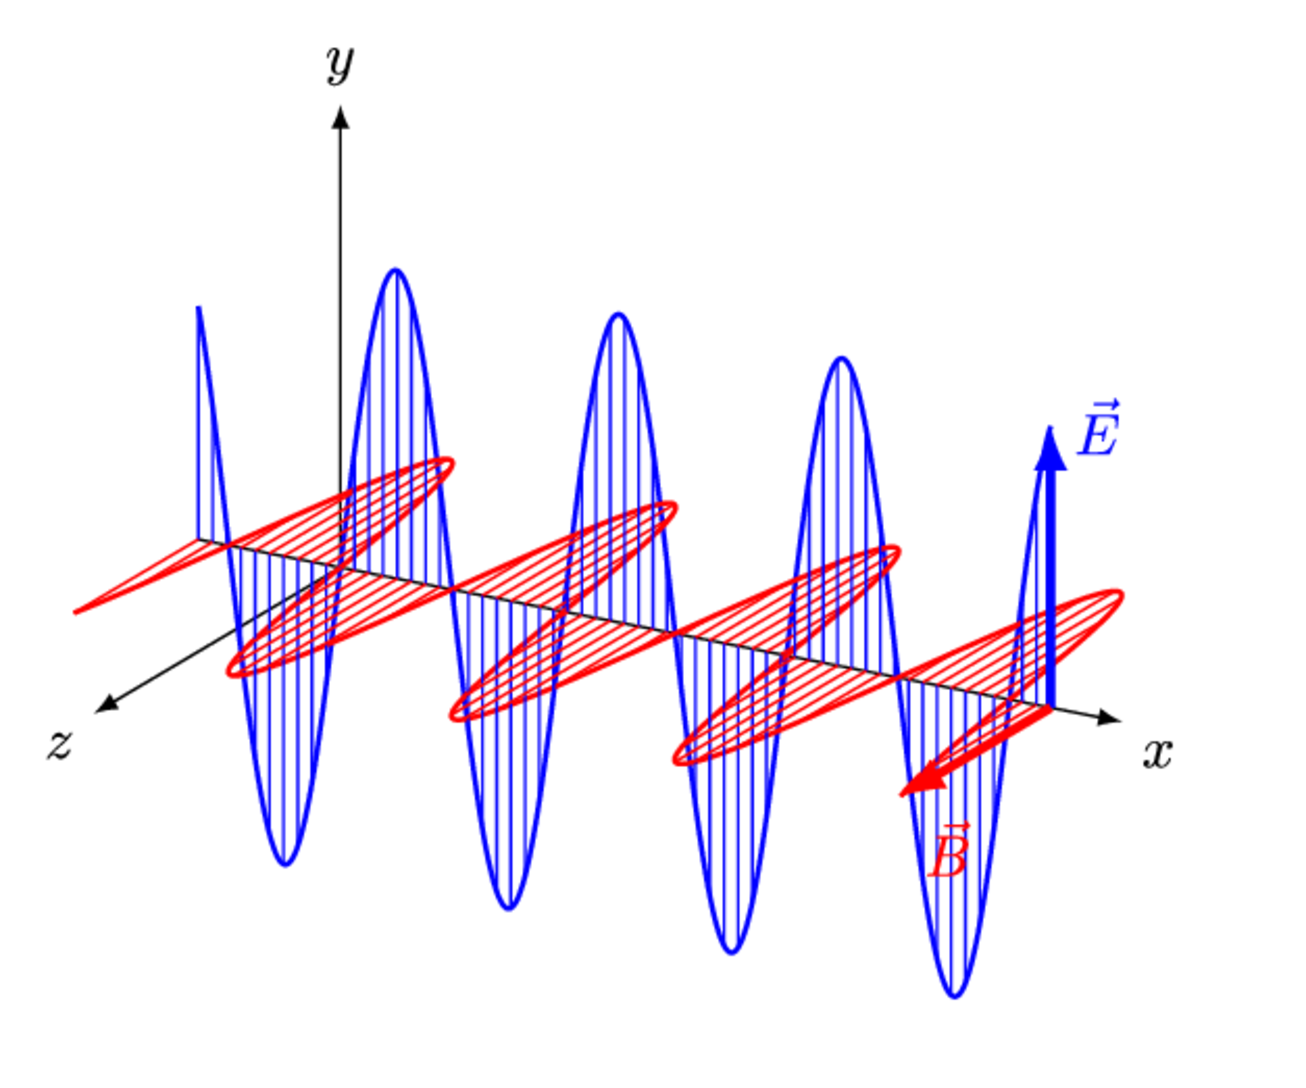
\includegraphics[width=0.6\linewidth]{images/EM-Wave} 

}

\caption{The orthogonal electric and magnetic oscillating fields of plan polarised light, propagating along the x-axis. From: [And1mu](https://upload.wikimedia.org/wikipedia/commons/9/99/EM-Wave.gif) / [CC BY-SA](https://creativecommons.org/licenses/by-sa/4.0)}\label{fig:EMWave}
\end{figure}

\hypertarget{sec:Light}{%
\section{Light}\label{sec:Light}}

As you've already learnt light exhibits properties that have both a wave like and a particle like nature, and light was one of the fundamental pieces that lead towards the quantum theory of the atom. Newton had shown that light from the sun is comprised of a spectrum of colours, we now know that that spectrum goes beyond what we can see with our eyes.

\begin{figure}
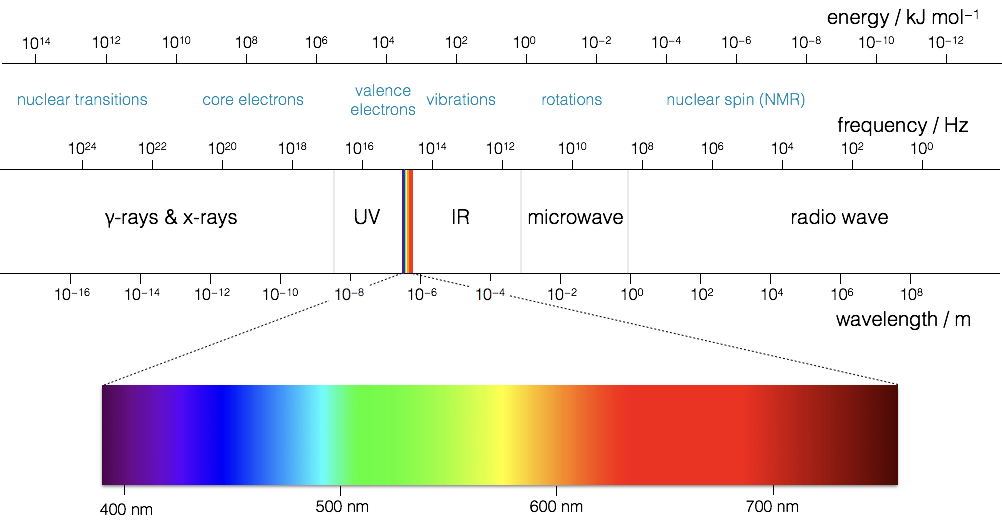
\includegraphics[width=1\linewidth]{images/EMspectrumspectroscopy} \caption{TheThe electromagnetic spectrum of light, frequency and energy are equivalent, so high frequency waves have high energy photons}\label{fig:EMspect}
\end{figure}

In your studies you have already seen how large amounts of the electromagnetic spectrum is used for different spectroscopic techniques, making use of the quantised transitions within molecules. For example, infra-red light has the same energy as the vibrational transitions within molecules. In photochemistry, we are specifically interested in the visible and near UV part of the EM spectra as photons with this energy promote transitions for the valance electrons in the molecules we are interested in.

It is important never to forget the wave particle duality of light, however for much of photochemistry and photophysics it is perhaps simpler to consider the light as a stream of incident photons.

\hypertarget{ch:Abs}{%
\chapter{Absorption of light}\label{ch:Abs}}

\hypertarget{sec:AbsLOs}{%
\subsection{Learning Objectives}\label{sec:AbsLOs}}

At the end of this section you should be able to:

\begin{itemize}
\tightlist
\item
  Appreciate changes in molecular geometry brought about by light absorption
\item
  Use the Beer Lambert Law to calculate light absorption
\item
  Discuss electronic transitions in terms of Morse energy curves
\item
  Explain the Franck Condon principle and Franck Condon factors
\item
  List selection rules for excitation of a photon and describe factors which affect the molar extinction coefficient
\end{itemize}

There is a Concept Bite video in Section \ref{sec:before1} which summarises much of this content.

\hypertarget{sec:AbsIntro}{%
\section{Introduction}\label{sec:AbsIntro}}

As you have previously learnt energy levels are quantised, in other words atoms and molecules can only have defined amounts of energy. Different transitions (electronic, vibrational, rotational) in atoms and molecules use different characteristic portions of the electromagnetic spectra, Figure \ref{fig:EMspect}.

When you saw atomic absorption and emission spectra the lines were very sharp, or in other words the absorption bands are very narrow as shown for the hydrogen absorption and emission spectra (figure \ref{fig:HAbsEm}).This isn't the case with molecular absorption spectra, particularly those in solution where absorption bands are typically hundreds of nanometers broad a typical organic fluorophor is shown in figure \ref{fig:RhoAbsEm}.The broad nature of the bands in molecular systems is a product of many individual factors including solvation, vibrational \& rotational factors and non minimised structural configurations.

\begin{figure}

{\centering 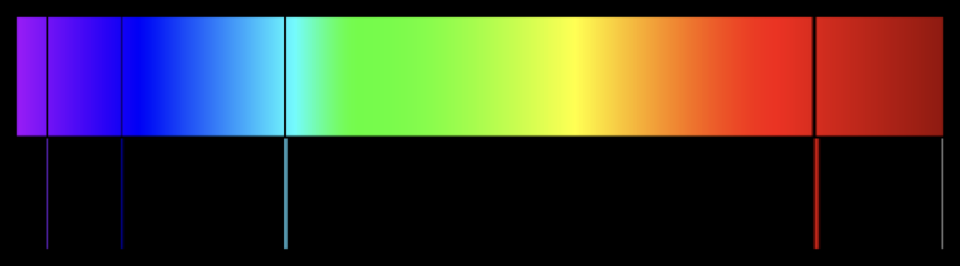
\includegraphics[width=0.7\linewidth]{images/HAbsEm} 

}

\caption{The absorption (top) and emission (bottom) spectra of hydrogen showing the very narrow band features, [image](http://montessorimuddle.org/2012/02/01/emission-spectra-how-atoms-emit-and-absorb-light/) adapted from [Adrignola](https://commons.wikimedia.org/wiki/User:Adrignola) licensed under CC BY 2.0}\label{fig:HAbsEm}
\end{figure}

\begin{figure}

{\centering 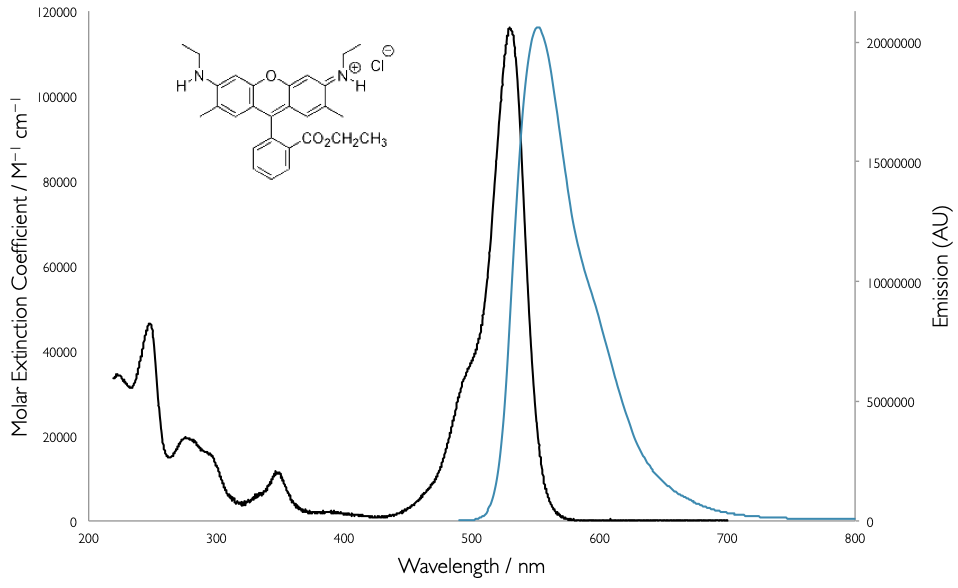
\includegraphics[width=0.6\linewidth]{images/Rhodamine6GAbsEm} 

}

\caption{The absorption (black) and emission (teal) spectra of Rhodamine 6G in ethanol. The emission spectra was recorded with an excitation wavelength of 480 nm and a bandwidth of 4.25 nm [Adapted from [OMLC](https://omlc.org/spectra/PhotochemCAD/html/083.html), [2nd July 2014]]}\label{fig:RhoAbsEm}
\end{figure}

\hypertarget{sec:BeerLambert}{%
\section{Beer-Lambert Law}\label{sec:BeerLambert}}

The empirical equation (equation \eqref{eq:BeerLambert}, figure \ref{fig:BeerLambert}) implies that the probability of a photon being absorbed at any point is the same (much like first order kinetics), and the amount of the total absorption depends upon the the concentration of the sample, c, and the `path length', l.

The amount of absorbance, A, is dependent upon the wavelength of the incident light, and the constant of proportionality, \(\varepsilon\) (here called the molar extinction coefficient), is consequently also wavelength dependent.
\begin{equation}
\log \frac{I_0}{I}=A=\varepsilon cl
\label{eq:BeerLambert}
\end{equation}

The wavelength of a particular value of the molar exctinction coefficient is often represted as a subscript, \(\varepsilon _\lambda\)

\begin{figure}

{\centering 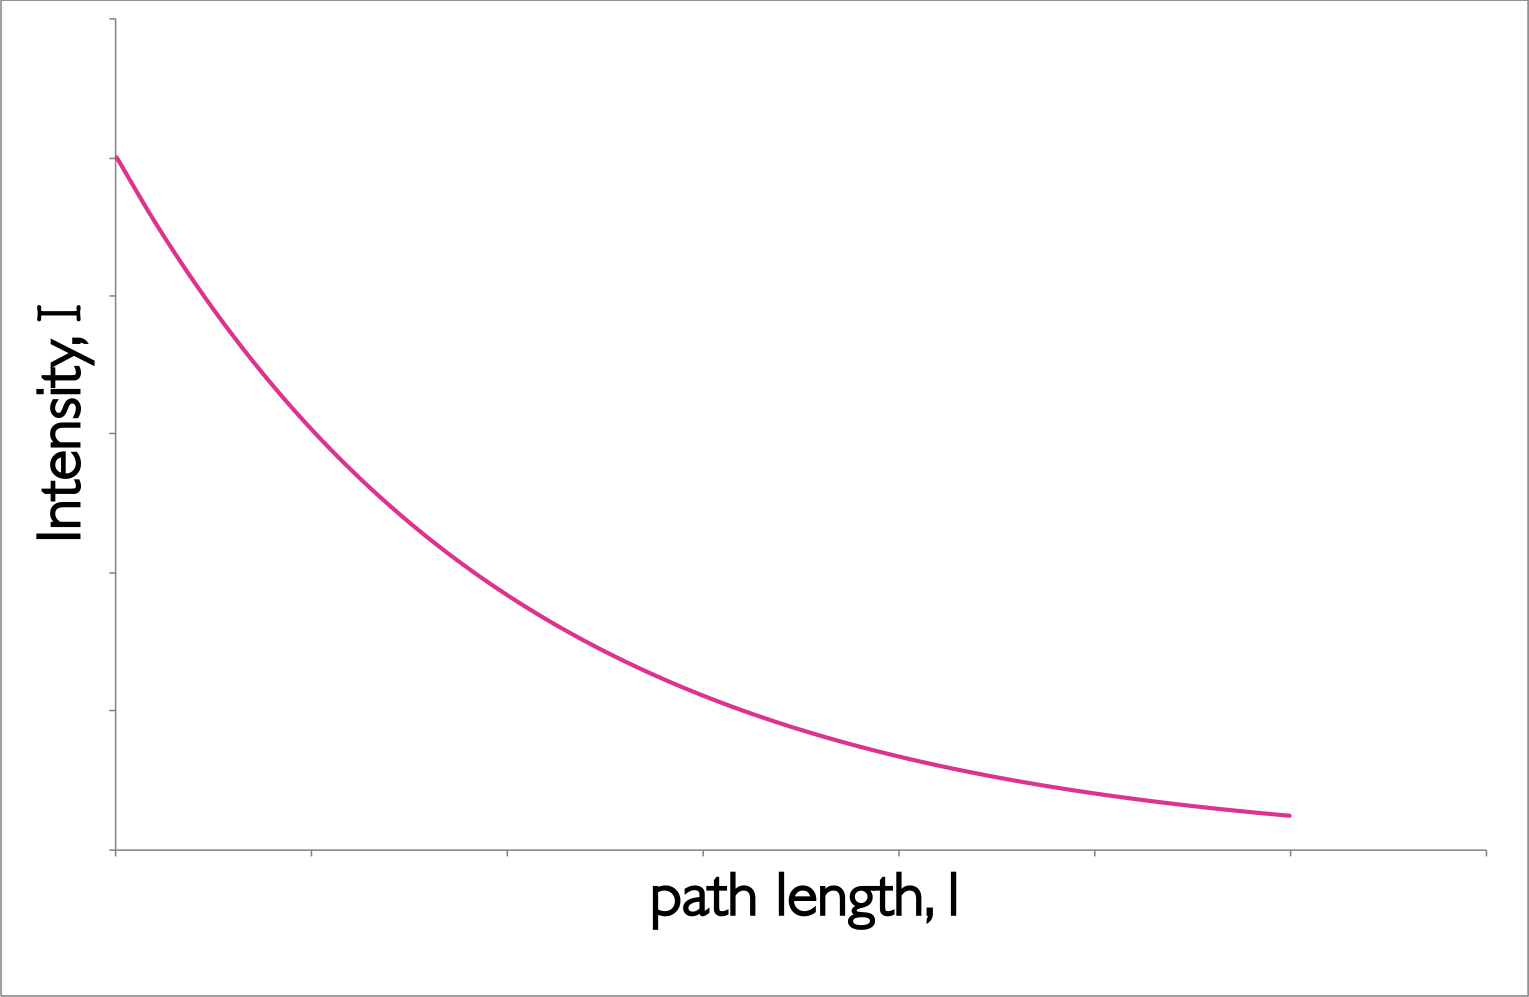
\includegraphics[width=0.5\linewidth]{images/BeerLambert} 

}

\caption{The decay of intensity of monochromatic incident light through a uniformly absorbing medium. The decay follows an exponential pattern as elucidated in the Beer-Lambert equation.}\label{fig:BeerLambert}
\end{figure}

The Beer-Lambert law makes a number of assumptions, and this exponential decay of the intensity of light is an important factor.When using the Beer-Lambert law you consider the intensity of the incident radiation, there is an assumption that the intensity of the radiation reaching each part of the sample does not deviate much from this. Hence high absorbing samples tend to show strong deviation from the Beer-Lambert's linear relationship.

The Beer-Lambert law also has to make a number of other `reasonable' considerations:

\begin{itemize}
\tightlist
\item
  The solutions is well mixed, and absorbers are homogeneously distributed in solution.
\item
  The absorbers do not scatter radiation (all particles will Rayleigh and Raman scatter but this is normally considerably less intense than absorption). Consequently solutions should be optically transparent as optically opaque solutions (such as colloidal solutions) have considerably stronger scattering.
\item
  The absorbers acts independently of each other, this means solutions need to be at a reasonably low concentration (typically less than 0.01 M, or maybe even less depending on the species) so as to avoid electrostatic or \(\pi\) stacking interactions between the chromophores.This is in part important because light is only absorbed when the polarisation of the light is aligned with the transition dipole moment.
\item
  The incident radiation is collimated, and each photon should pass through the same path length.
\item
  The sample holder (cuvette) is optically `pure' such that reflections are avoided (linked to the assumption above).
\item
  The incident radiation is monochromatic, or at the very least has a band width more narrow than the band width of the absorbing transition (this is usually not an issue for molecular systems as bandwidths are usually 10s or more of nm wide, but for atomic or ion spectroscopy where bandwidths are \textless0.02 nm this is a factor which must be carefully considered.
\item
  The incident radiation does not noticeably affect the concentration of the ground state, in other words the amount of excited states generated must be kept small as when we are talking about the absorption of a chromophore the concentration of that chromophore that appears in the Beer-Lambert equation is the ground state concentration.
\item
  There is no measurable emission from the sample.
\end{itemize}

However, this empirical relationship can be examined in a deeper way.

\hypertarget{sec:MOs}{%
\section{Molecular orbitals, HOMO \& LUMO}\label{sec:MOs}}

Ultimately, the absorption (and emission of a photon) which can be modelled empirically, as in the Beer-Lambert lawn, is actually a property of the quantum mechanics of the system as indicated by the models of absorption and emission of photons by Einstein.

If we think about the size of an atom or molecule (atoms are 100s of pm, molecules frequently less than 1 nm) they are considerably smaller than the wavelength of light required for electronic transitions, so it is often easier to think of an entirely photonic model of light.

If we considered the atom or molecules to be formed of a cloud of electrons bathed in the electromagnetic field, the electron density is attracted to the the positive side of the field, and the positively charged nucleus to the negative side. However, electrons are much lighter (about 1/1760 the mass of a a proton) and so it is the lighter electrons that `feel' the most effect. As the electric field oscillates it pushes and pulls the electrons within the molecule.

This transition is called an electric-dipole transition since it either creates (absorption) or destroys (emission) an oscillating electric dipole in the atom or molecule.The transition dipole moment, \(\mu_i\), arises from the charge displacement during the transition. The magnitude of this transition dipole moment depends upon the distance the net electronic charge is moved from the ground state average position. This transition dipole is entirely independent of any permanent dipole moment within the molecule.

Figure \ref{fig:Butadiene} shows the valence molecular orbitals of butadiene, showing the discrete energy levels in the system, absorption of a photon allows an electron to be excited from the highest occupied molecular orbital (HOMO) to any excited state.

Upon excitation of an electron there is a mixing of the molecular orbitals of the fully and partially occupied molecular orbitals, in the case of butadiene excitation of an electron from the HOMO to the LUMO (lowest unoccupied molecular orbital), giving the central C-C bond some double bond character, limiting rotation and leading to a structural change of the excited state.

\begin{figure}

{\centering 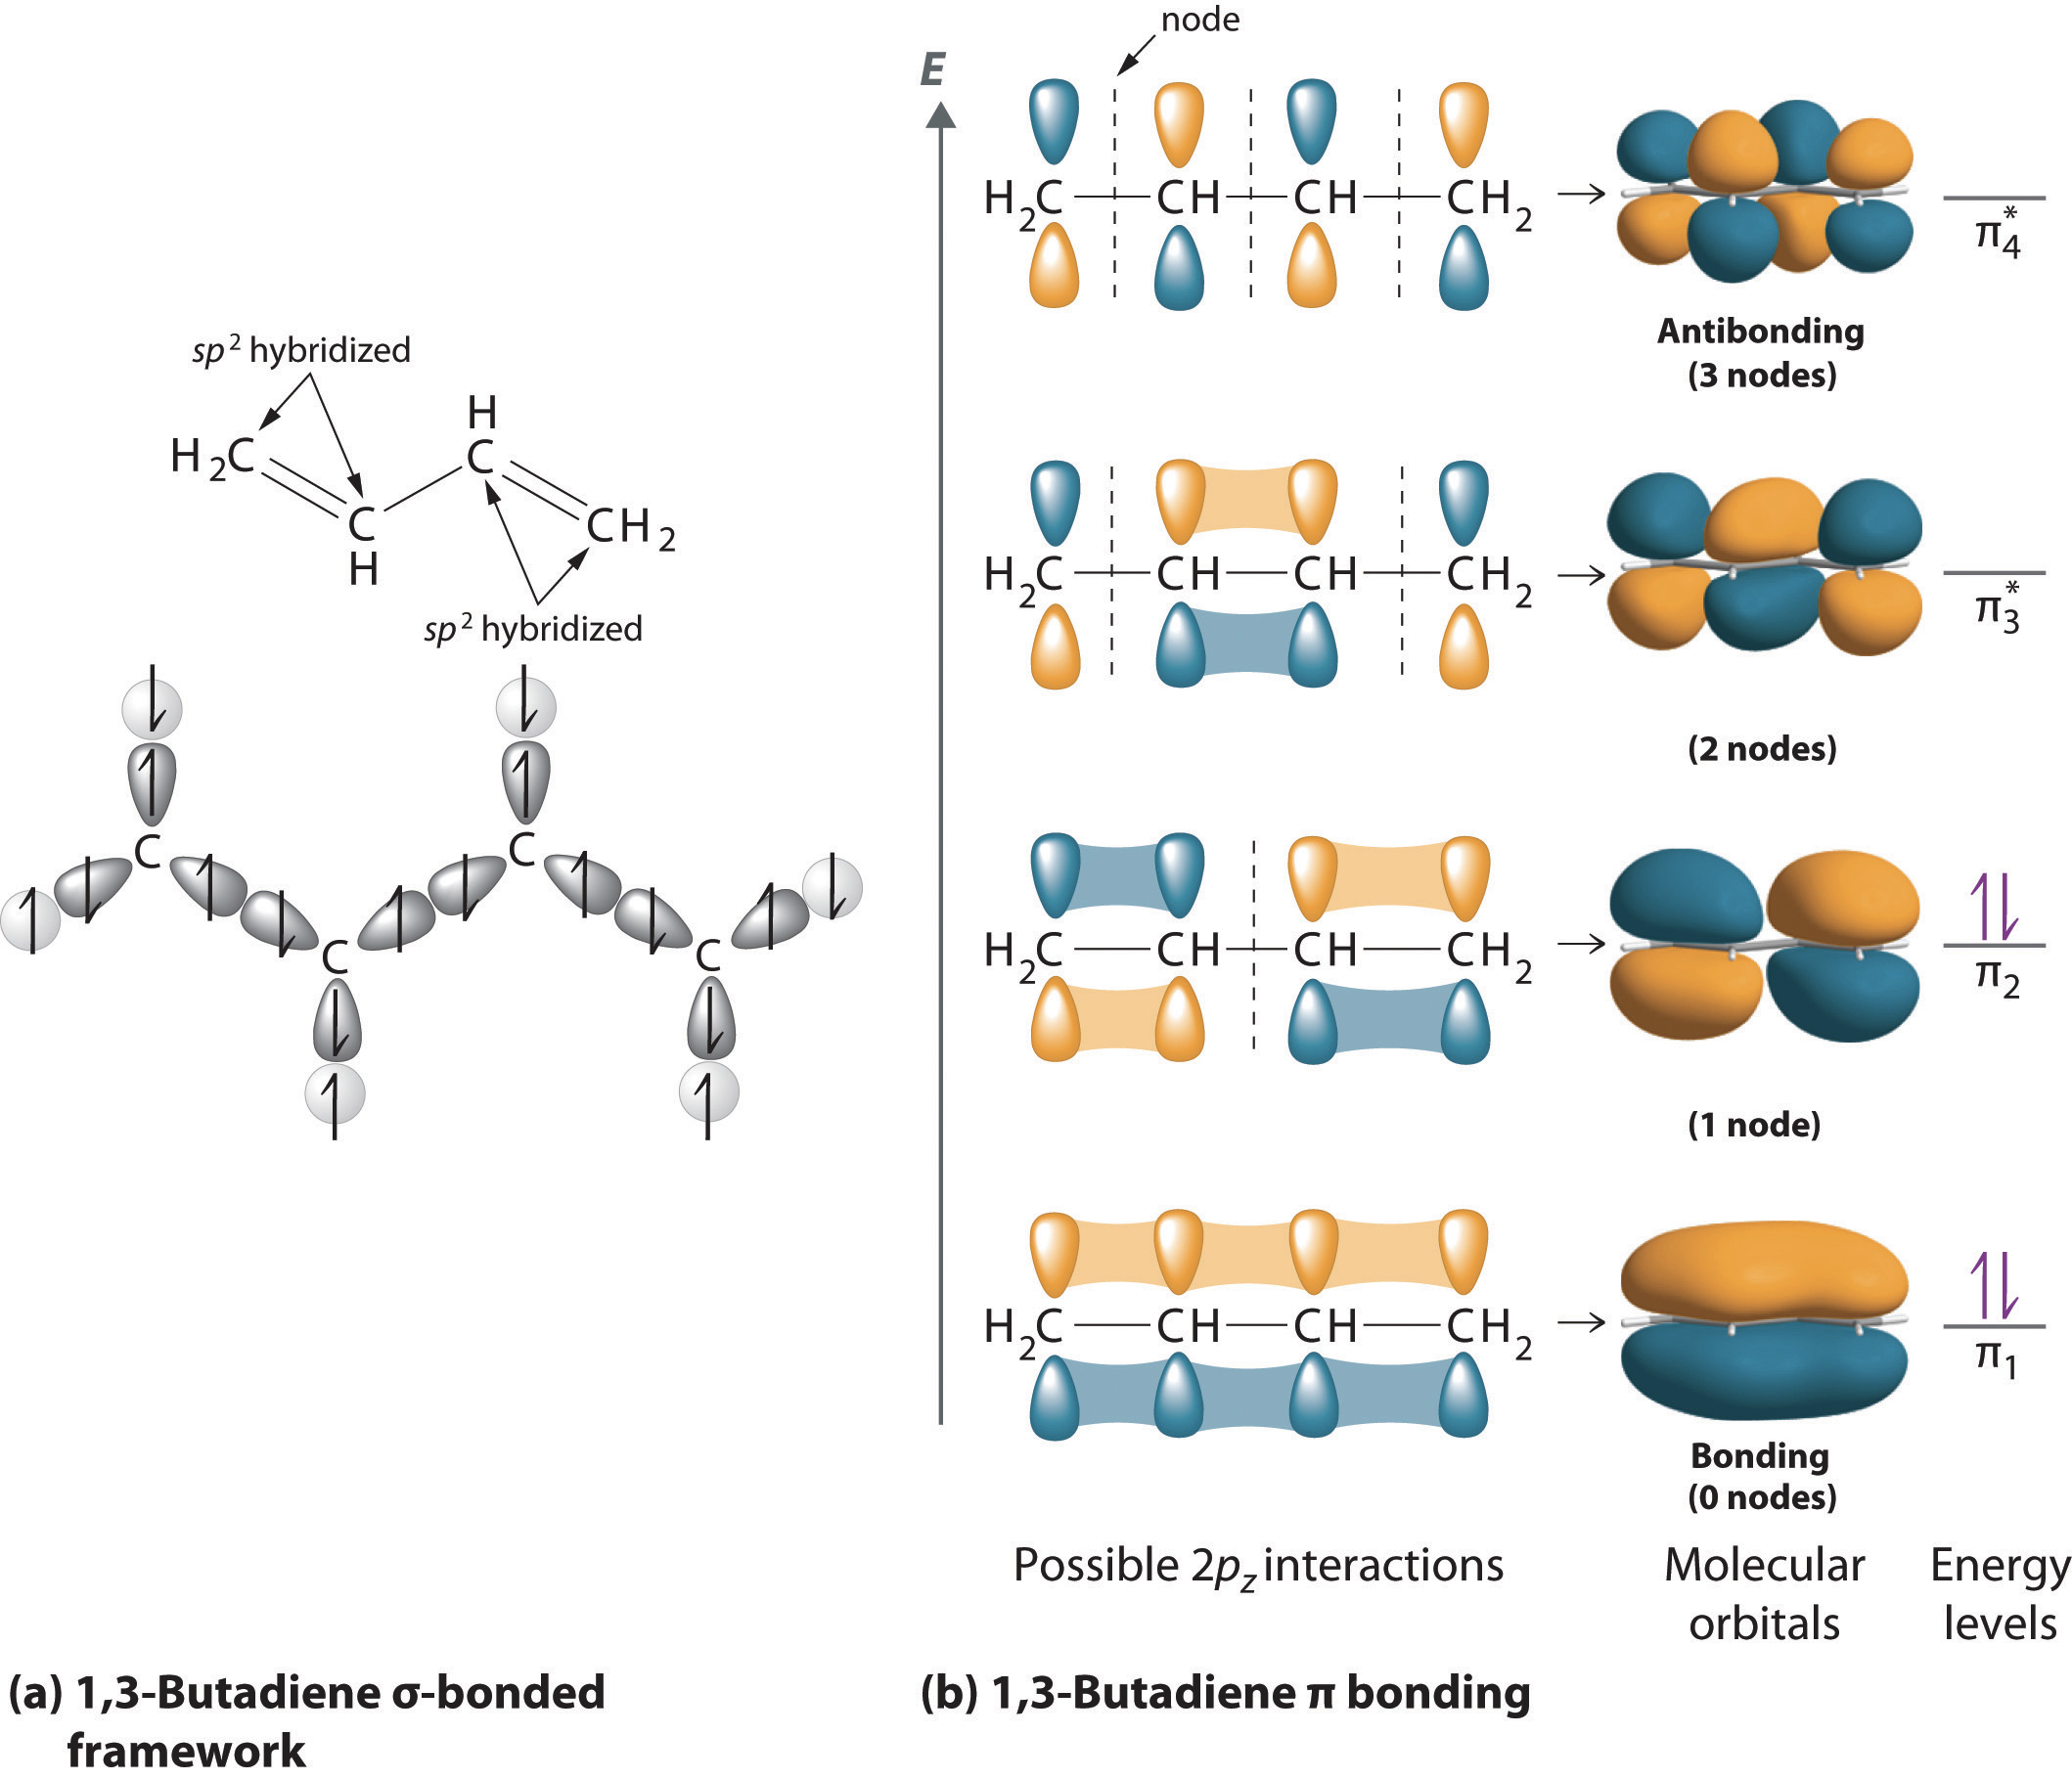
\includegraphics[width=0.7\linewidth]{images/Butadiene} 

}

\caption{MO diagram of butadiene, each carbon atom is assumed to be sp$^2$ hybridised, with linear combination of the 2p$_z$ orbitals. As the energy of the levels increases so does the number of nodes. The lowest two energy levels are fully occupied in the ground state, upon absorption of a photon an electron is promoted to one of the anti-bonding orbitals allowing rotation around the double bonds, and giving the centre single bond some double bond character. [[MO diagram of butadiene](https://2012books.lardbucket.org/books/principles-of-general-chemistry-v1.0m/s13-04-polyatomic-systems-with-multip.html). From by Averill \& Eldredge, Principles of General Chemistry licensed under CC BY 2.0. Sept 14.]}\label{fig:Butadiene}
\end{figure}

In simple organic molecules we only really need to consider \(\pi\) and \(\pi^\ast\) and \(n\) (non-bonding) molecular orbitals as the energy difference between \(\sigma\) and \(\sigma^\ast\) orbitals are comparatively very large.

The process of absorption of a photon is very fast (\textasciitilde1 fs) (compared with the timescales of vibrations in molecule (\textasciitilde10 ps)), this is the basis of the Franck-Condon principle. Consequently when absorption (and emission) processes are sketched, as in figure \ref{fig:FrankCondon}, absorption and emission can be indicated by vertical transitions.

The `strength' of the absorption transition, which relates to the extinction coefficient in the Beer-Lambert law, and the Einstein \(B\) coefficient is in fact a measure of the `overlap integral' of the wave functions of the ground and excited states.

\begin{figure}

{\centering 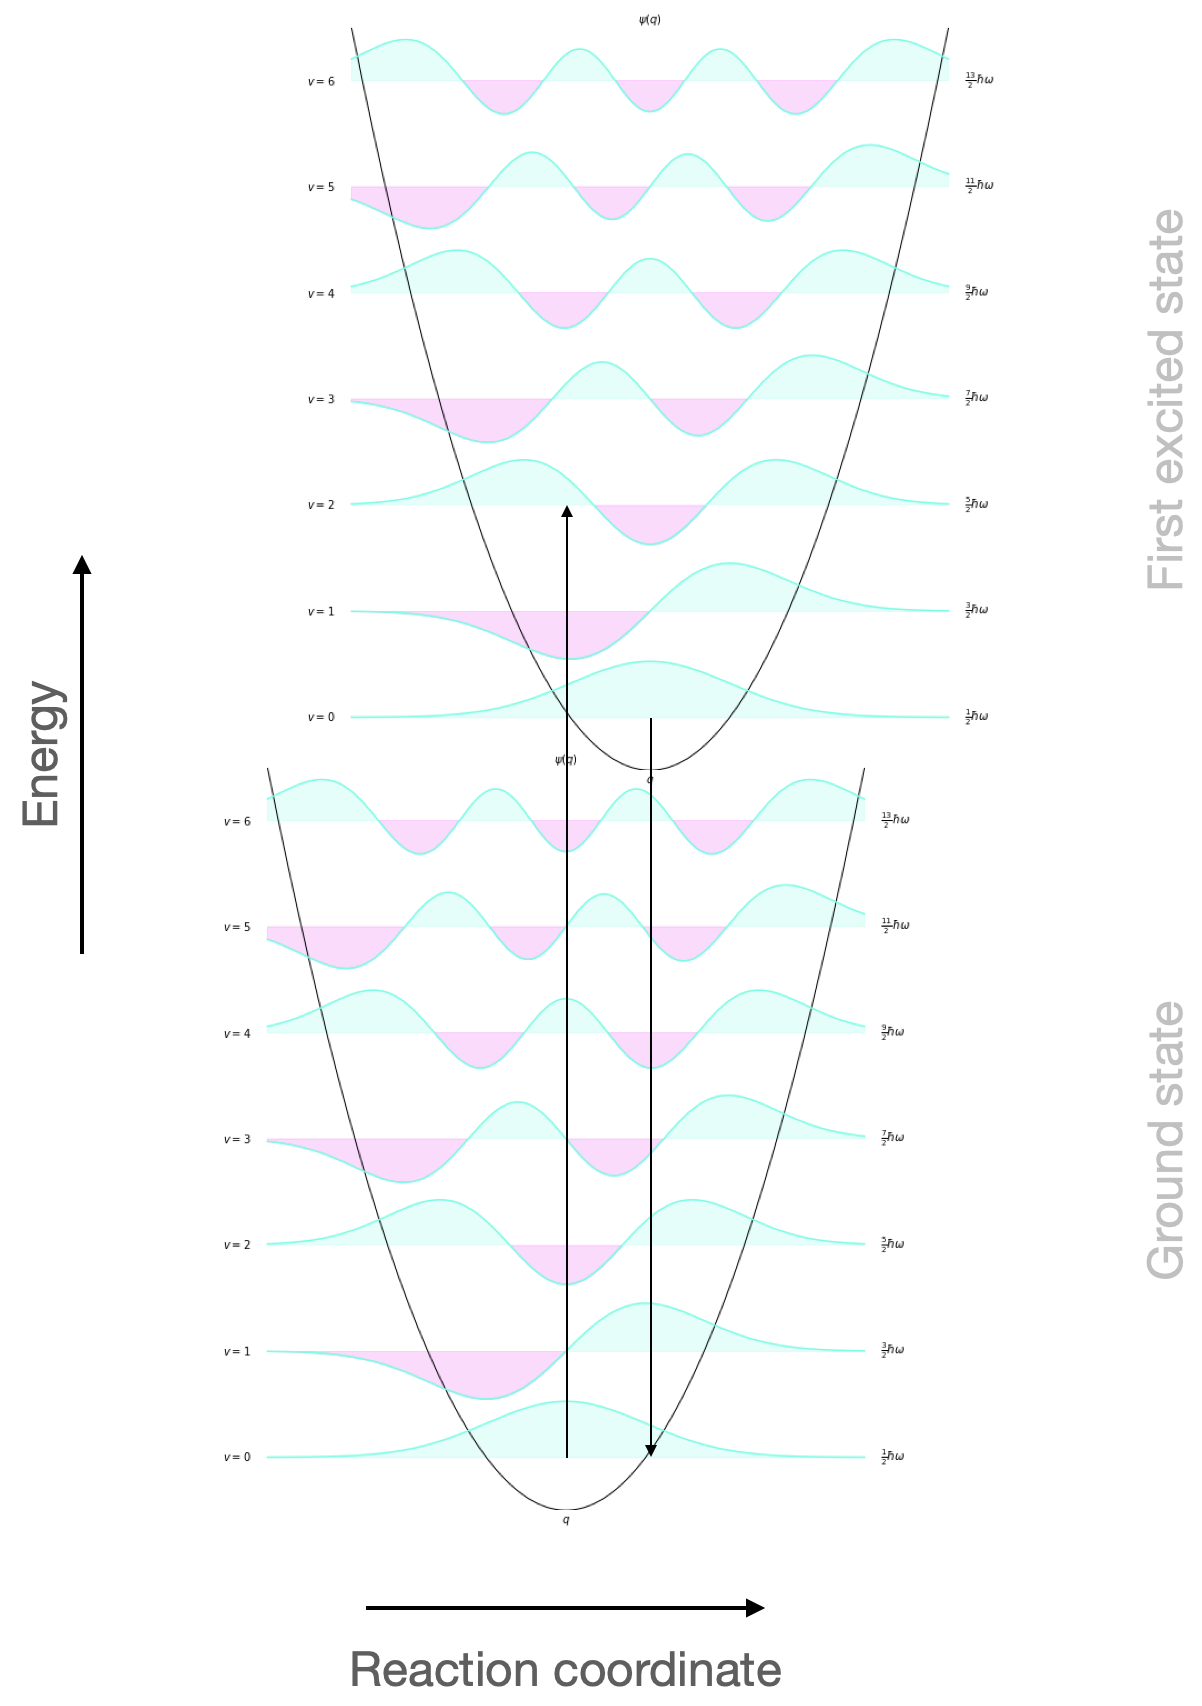
\includegraphics[width=0.6\linewidth]{images/FrankCondon} 

}

\caption{The vertical line of the absorption transition as the electron is promoted from the ground state to the excited state. The probability of the electron being excited into each vibrational level is given by the ‘overlap’ of the wave functions of ground and each excited state. [[Franck-Condon Diagram](https://commons.wikimedia.org/wiki/File:Franck-Condon-diagram.png). From Wikimedia Commons, created by [Mark M. Somoza](http://www.gnu.org/licenses/fdl-1.3.html), CC-BY-SA-[3.0](https://creativecommons.org/licenses/by-sa/3.0/). Sept 14. ]}\label{fig:FrankCondon}
\end{figure}

The greater the overlap integral between the ground and excited state the higher the molar extinction coefficient and the more strongly coloured the molecule.

Understanding the variation of possible electronic transitions available when electronic levels are mixed with vibrational and rotational levels, as well as the molecular dynamics allowing multiple `non-minimised' structures explains the relative broadness of molecular electronic absorption and emission spectra.

\begin{figure}

{\centering 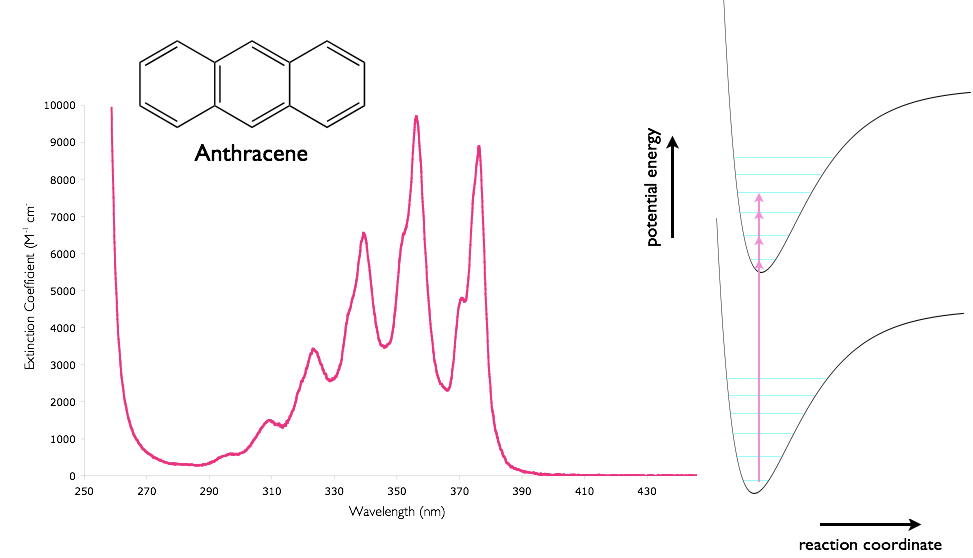
\includegraphics[width=0.9\linewidth]{images/Anthracene} 

}

\caption{The absorption spectra of anthracene in cyclohexane showing the vibrational fine structure, combined with a sketch of the potential energy wells of the ground and excited states. Regions with the highest molar extinction coefficient have the largest overlap integrals of the wavefunctions of the ground and excited states. }\label{fig:Anthracene}
\end{figure}

\hypertarget{sec:multiplicity}{%
\section{Multiplicity}\label{sec:multiplicity}}

If you recall Hunds' rule when filling atomic and molecular orbitals you will recall that the lowest energy state occurs when the spin of the electrons is aligned. Usually in an organic molecular orbital the HOMO is a fully occupied \(\pi\) set, or a fully occupied set of non bonding orbitals with all electrons paired.

It is common to refer to the electronic states in a molecule by their \emph{spin multiplicity}, given by \(2S+1\), where \(S\) is the sum of the electronic spins of the electrons in the orbital. For a species in which all of the electrons are paired \(S = 0\), and so \(2S+1 = 1\) and the state is referred to as a \emph{singlet}.

If two electrons are unpaired they will (in the lowest energy configuration) have parallel spins, the total spin \(S = 1\) and so the spin multiplicity, \(2S + 1 = 3\). This state is referred to as a \emph{triplet} state.

Species such as free radicals have one unpaired electron, consequently \(S = ½\), and \(2S + 1 = 2\), and the species is referred to as a \emph{doublet}.

Triplet states with the same electronic configuration (other than spin) have a lower energy than corresponding singlet states due to an effect called spin correlation. In triplet states the motion of the electrons in the orbitals are organised in such a way as to minimise the coulombic interactions between the charges, by minimising these coulombic interactions the energy of the system is also lowered.

Although formally flipping of electron spin is forbidden in photophysical and non photophysical processes it does occur. Processes that involve a change in electron spin are explained in later sections.

\hypertarget{sec:conjugationandenergygap}{%
\section{\texorpdfstring{Conjugation and the HOMO, LUMO energy gap, \(\Delta E\)}{Conjugation and the HOMO, LUMO energy gap, \textbackslash Delta E}}\label{sec:conjugationandenergygap}}

\begin{figure}

{\centering 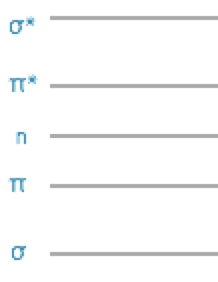
\includegraphics[width=0.2\linewidth]{images/nPiSigmaenergylevels} 

}

\caption{The relative energy arrangement of orbitals in a molecule, this simple sketch is usually good enough to gain an understanding of the system under investigation.}\label{fig:EnergyLevels}
\end{figure}

The greater the amount of conjugation in a molecule the smaller the energy gap between the HOMO \& LUMO and the longer the wavelength of photon absorbed.

This fits with the theory you learnt in your quantum mechanics lectures, where you can model the linear conjugated model quite accurately using the particle in a one dimensional box model.

\begin{longtable}[]{@{}llll@{}}
\caption{\label{tab:lambdaconj} The dependence of maximum absorption wavelength on the increasing length of conjugation is clearly shown by moving along the diene, triene, polyene series. Inclusion of a hetero atom with lone pairs introduces non-bonding, \(n\), electrons into the MO, and a second absorption band \(n \longrightarrow \pi^\ast\) introduced with a lower energy transition.}\tabularnewline
\toprule
\begin{minipage}[b]{0.22\columnwidth}\raggedright
\strut
\end{minipage} & \begin{minipage}[b]{0.22\columnwidth}\raggedright
\(\lambda\)\textsubscript{max} / nm \(\pi \longrightarrow \pi^\ast\)\strut
\end{minipage} & \begin{minipage}[b]{0.22\columnwidth}\raggedright
\strut
\end{minipage} & \begin{minipage}[b]{0.22\columnwidth}\raggedright
\(\lambda\)\textsubscript{max} / nm \(n \longrightarrow \pi^\ast\) \(\pi \longrightarrow \pi^\ast\)\strut
\end{minipage}\tabularnewline
\midrule
\endfirsthead
\toprule
\begin{minipage}[b]{0.22\columnwidth}\raggedright
\strut
\end{minipage} & \begin{minipage}[b]{0.22\columnwidth}\raggedright
\(\lambda\)\textsubscript{max} / nm \(\pi \longrightarrow \pi^\ast\)\strut
\end{minipage} & \begin{minipage}[b]{0.22\columnwidth}\raggedright
\strut
\end{minipage} & \begin{minipage}[b]{0.22\columnwidth}\raggedright
\(\lambda\)\textsubscript{max} / nm \(n \longrightarrow \pi^\ast\) \(\pi \longrightarrow \pi^\ast\)\strut
\end{minipage}\tabularnewline
\midrule
\endhead
\begin{minipage}[t]{0.22\columnwidth}\raggedright
\strut
\end{minipage} & \begin{minipage}[t]{0.22\columnwidth}\raggedright
217\strut
\end{minipage} & \begin{minipage}[t]{0.22\columnwidth}\raggedright
\strut
\end{minipage} & \begin{minipage}[t]{0.22\columnwidth}\raggedright
270 187\strut
\end{minipage}\tabularnewline
\begin{minipage}[t]{0.22\columnwidth}\raggedright
\strut
\end{minipage} & \begin{minipage}[t]{0.22\columnwidth}\raggedright
227\strut
\end{minipage} & \begin{minipage}[t]{0.22\columnwidth}\raggedright
\strut
\end{minipage} & \begin{minipage}[t]{0.22\columnwidth}\raggedright
\strut
\end{minipage}\tabularnewline
\begin{minipage}[t]{0.22\columnwidth}\raggedright
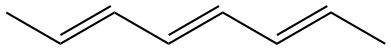
\includegraphics{images/octatrienestructure.png}\strut
\end{minipage} & \begin{minipage}[t]{0.22\columnwidth}\raggedright
263\strut
\end{minipage} & \begin{minipage}[t]{0.22\columnwidth}\raggedright
\strut
\end{minipage} & \begin{minipage}[t]{0.22\columnwidth}\raggedright
324 219\strut
\end{minipage}\tabularnewline
\begin{minipage}[t]{0.22\columnwidth}\raggedright
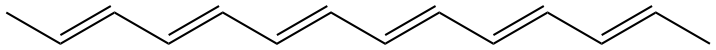
\includegraphics{images/longene.png}\strut
\end{minipage} & \begin{minipage}[t]{0.22\columnwidth}\raggedright
353\strut
\end{minipage} & \begin{minipage}[t]{0.22\columnwidth}\raggedright
\strut
\end{minipage} & \begin{minipage}[t]{0.22\columnwidth}\raggedright
\strut
\end{minipage}\tabularnewline
\bottomrule
\end{longtable}

\hypertarget{sec:selectionrules}{%
\section{Selection rules for absorption \& emission processes}\label{sec:selectionrules}}

In molecular systems the most important selection rule is \(\Delta S = 0\), or there can be no change in the spin multiplicity during an absorption or emission processes, or there can be no `flipping' of electrons spin during a transition. In practice `coupling' due to interactions between the spin of the electron and the orbital mean that this selection rule is not rigidly followed.

In organic molecules containing only C, H, N \& O the direct absorption from S\textsubscript{0} to T\textsubscript{1} is so weak that it can't be seen in the absorption spectra. This `spin-orbit coupling' is more pronounced for heavier elements and molecules containing particularly heavy atoms, such as S, Cl or Br have more relaxed adherence to the \(\Delta S = 0\) selection rule.

The Laporte selection rule is more relevant when looking at inorganic transition metal complexes, or for atomic spectra which will not be considered in this work. The Laporte states that there must be a change in angular momentum quantum number, \(l\), upon absorption or emission in a cento symmetric system, or \(\Delta l = \pm 1\). So in a centro symmetric molecule, such as {[}Ti(H\textsubscript{2}O)\textsubscript{6}{]}\textsuperscript{3+}, figure \ref{fig:Tisplitting}, the allowed transitions would be transitions such as the following:

\begin{equation*}
1s \longrightarrow 2p \hspace{2cm}\textrm{or} \hspace{2cm} 1s \longrightarrow 3p
\end{equation*}

Whilst these transitions would be forbidden according to the Laporte rule:

\begin{equation*}
1s \longrightarrow 2s \hspace{2cm}\textrm{or} \hspace{2cm} 1s \longrightarrow 3d
\end{equation*}

Consequently the \(d-d\) transitions, such as the \(t_{2g} \longleftrightarrow e_g\) transition in octahedral complexes, which give most transition metal complexes are forbidden according to the Laporte rule.

\textbackslash begin\{figure\}

\{\centering 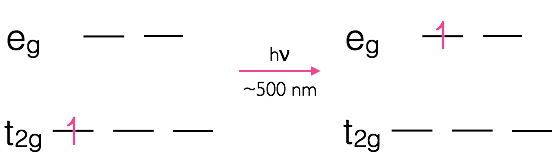
\includegraphics[width=0.6\linewidth]{images/Ti3splitting}

\}

\textbackslash caption\{The ligand field splitting of the 3d orbitals in a {[}Ti(H\(_2\)O)\$\_6{]}\(^{3+}\) complex the solution is pale purple with a molar extinction coefficient, ε \textasciitilde{} 6.1 M\textsuperscript{−1} cm\(^{−}1\)\}\label{fig:Tisplitting}
\textbackslash end\{figure\}

If we compare the magnitude of of the molar extinction coefficient for a typical \(d-d\) absorption of a transition metal complex with that of a `spin allowed' `Laporte allowed' organic dye molecule we can see the effect of `non allowed' transitions. In table \ref{tab:extcoeff}, the organics, DNA \& the synthetic dye TOTO-1 both have extended conjugated molecular orbitals, and the transitions are from singlet to singlet, an allowed transition.

In these cases the Laporte rule does not apply as there is no centre of symmetry. The two examples of transition metal complexes {[}Cu(H\textsubscript{2}O)\textsubscript{6}{]}\textsuperscript{2+} \& {[}Ti(H\textsubscript{2}O)\textsubscript{6}{]}\textsuperscript{3+}, have significantly lower molar extinction coefficients.

Molar extinction coefficients, if you recall, were a representation of the orbital overlap between the HOMO \& LUMO, or a measure of how `allowed' the transition is. The transitions which are Laporte forbidden are at least two orders of magnitude less intense than the allowed transitions of the organic molecules.

Interestingly, permanganate which is relatively highly coloured when compared to other transition metal complexes cannot have colour due to \(d-d\) transitions as the +7 oxidation state of the manganese ion leaves no electrons in either the \(s\) or \(d\) orbitals. Instead the colour is due to a charge transfer transition, where upon absorption of a photon an electron is briefly transferred from one of the oxygen ligands to the manganese metal centre. Ligand to metal charge transfer complexes (and the associated metal to ligand charge transfer complexes), are not subject to selection rules and so are relatively intense.

\begin{longtable}[]{@{}lll@{}}
\caption{\label{tab:extcoeff} The molar extinction coefficients of a range of molecules, the magnitude is strongly dependent upon the adherence to selection rules, the two organic molecules, DNA bases \& TOTO-1 are both `spin allowed', permanganate is a LMCT which has no selection rules, whereas the final three molecules all fall foul of the Laporte selection rule which states \(\Delta l = \pm 1\). Since these transitions are `forbidden' the molar extinction coefficient is considerably lower than the allowed transitions.}\tabularnewline
\toprule
& \(\lambda\)\textsubscript{max} / nm & \(\varepsilon _{\lambda}\) / M\textsuperscript{-1} cm\textsuperscript{-1}\tabularnewline
\midrule
\endfirsthead
\toprule
& \(\lambda\)\textsubscript{max} / nm & \(\varepsilon _{\lambda}\) / M\textsuperscript{-1} cm\textsuperscript{-1}\tabularnewline
\midrule
\endhead
DNA (per base) & 260 & 6600\tabularnewline
TOTO-1 & 514 & 117000\tabularnewline
KMnO\textsubscript{4} & 520 & 1800\tabularnewline
CuSO\textsubscript{4} & 810 & 20\tabularnewline
{[}Ti(H\textsubscript{2}O)\textsubscript{6}{]}\textsuperscript{3+} & 500 & 6.1\tabularnewline
PrCl\textsubscript{3} & 445 & 0.07\tabularnewline
\bottomrule
\end{longtable}

The weak absorption carries on for the lanthanide complexes where \(f-f\) transitions are again forbidden by the Laporte selection rule. However, Ce\textsuperscript{3+} and Tb\textsuperscript{3+} have more intense electronic absorption bands which appear in the UV.

These are due to {[}Xe{]}4\(f\)\textsuperscript{n} to {[}Xe{]}4\(f\)\textsuperscript{n-1}5\(d\)\textsuperscript{1} transitions. Since the electron is moving from an \(f\) orbital to an \(d\) orbital it is not forbidden by the Laporte selection rule and so is considerably more intense than the forbidden \(f-f\) transitions. These transitions occur for these to ions due tooth stability provided by either an empty of half filled subshell.

\hypertarget{sec:structureonabs}{%
\section{Structure and Bonding Upon Absorption of a Photon}\label{sec:structureonabs}}

\begin{figure}

{\centering 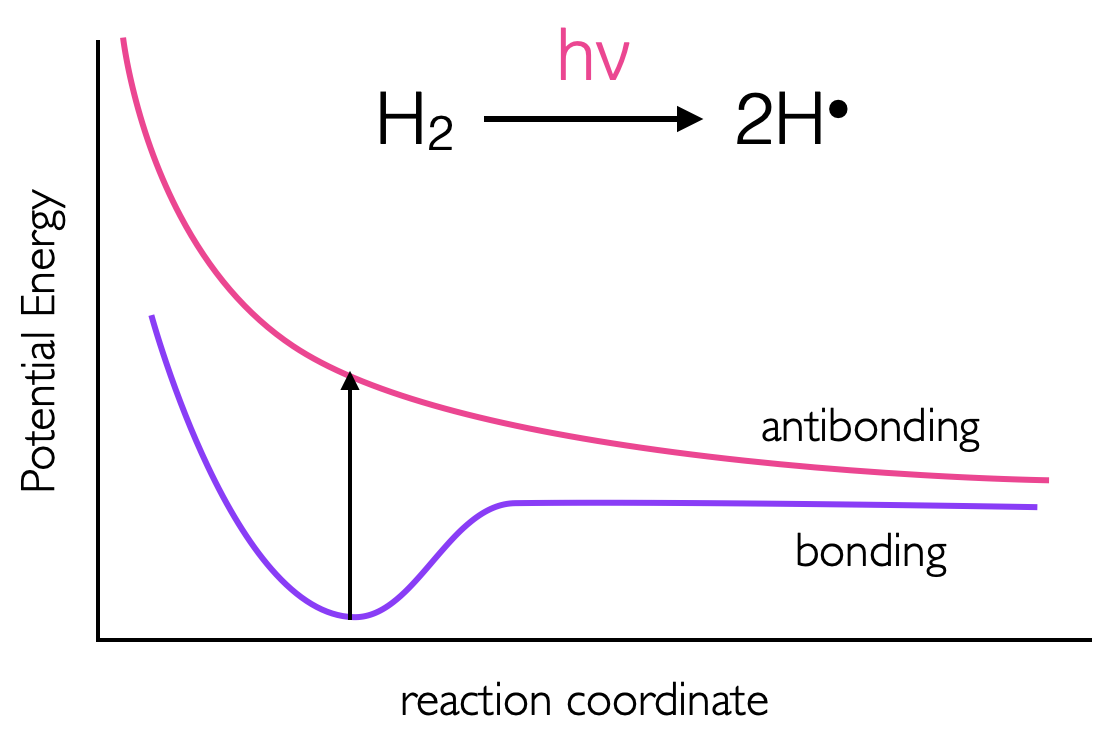
\includegraphics[width=0.6\linewidth]{images/Hbondingen} 

}

\caption{The energies of  bonding and anti bonding orbitals of molecular hydrogen, as an electron is prompted to the anti bonding σ* orbital the bond order is reduced to zero and the molecule ‘falls apart’..}\label{fig:Hbondingen}
\end{figure}

\begin{figure}

{\centering 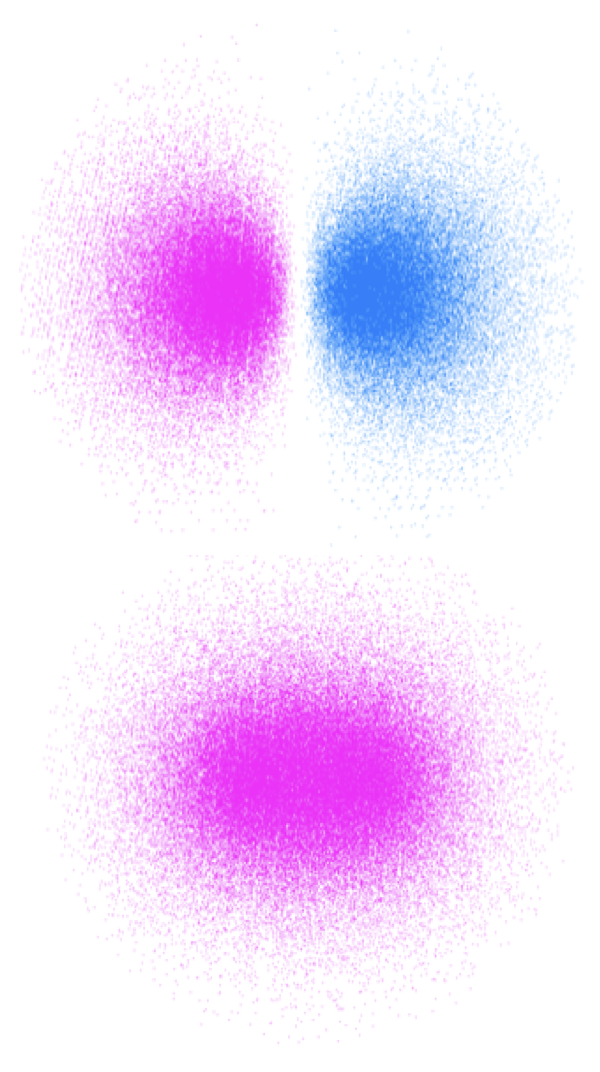
\includegraphics[width=0.3\linewidth]{images/Hbondingorb} 

}

\caption{The bonding and anti bonding orbitals of molecular hydrogen showing the node along the σ bond for the anti-bonding orbital.}\label{fig:Hbondingorb}
\end{figure}

Upon absorption of a photon, if an electron is promoted to an anti bonding orbital there is a reduction in the bond order. For a hydrogen molecule, with just two electrons, this leads to radical formation figures \ref{fig:Hbondingen} \& \ref{fig:Hbondingorb}.
It should be remembered that there is still an electron in the bonding orbital and the molecular orbital is now a blend of the HOMO and LUMO. The LUMO
For molecules with \(\pi\) electrons excitation of an electron to a \(\pi ^\ast\) orbital reduces the bond order to just 1, allowing for rotation around the previously restricted bond. If ethene is excited, the sp\textsuperscript{2} hybridised carbon, takes upon character of sp\textsuperscript{3} allowing rotation around the C-C bond, and changing the H-C-H bond angles. Rotation around a double bond is the basis of many photochemical reactions and is fundamental to vision where retinol, a long conjugated molecule undergoes a cis-trans isomerisation after excitation.

\hypertarget{sec:transdipole}{%
\section{The Transition Dipole Moment}\label{sec:transdipole}}

One thing which hasn't yet been considered is how light physically interacts with a molecule.

Classically it could be considered that the oscillating electric field of a wave could interact with a molecule if there was some resonance of the of the frequency of light and the frequency of oscillation of the electron in an orbital, it would seem obvious that an electron (carrying an electric charge) and an electromagnetic wave (with its oscillating electric field) should interact; and will interact given the correct wavelength. In simple terms the frequency of light and the energy gap for the transition were the same.

The classical model also explains why it is electrons which are excited (and not protons in the nucleus) because the considerably lighter electrons are more affected (and moved more) in the presence of the electric field.

This approach whilst covering the very basics of a transition does not particularly explain concepts such as the molar extinction coefficient, nor does it particularly consider concepts fundamental to quantum mechanics - such as quantisation of energy - an oscillating electric field is in no way quantised and there is no reason why excitation of the molecule should be quantised either.

However this idea of an oscillating dipole has some relation to quantum mechanics; because the shape of the molecular orbitals of the HOMO and LUMO are different and there will be a change in the electron distribution and hence a change in dipole of the molecule upon excitation. As such we can define a transition dipole moment for each chromophore - the more similar the ground and excited states the larger the transition dipole moment for the molecule.

A mathematical derivation of the transition dipole moment is beyond the scope of this work\footnote{see Principles of Photochemistry by Turro \emph{et al} if you wish to know more}, but it is worth discussing as transition dipoles are hugely important when it come to energy transfer in molecules (see Förster Resonance energy transfer, Section @ref(\{sec:forster\}).

If we consider light as a wave polarisation is well understood, however there is a quantum mechanical explanation for polarisation as well - in short we can use wave behaviour to consider polarisation and photon behaviour to explain quantisation - just to stick with concepts which should be familiar to us.

Light is only absorbed by a molecule if the polarisation of the light aligns with the transition dipole moment on the molecule. Figure \ref{fig:CS2} shows CS\textsubscript{2} a simple linear molecule - where the transition dipole moment runs along the long axis of the molecule.

\begin{figure}

{\centering 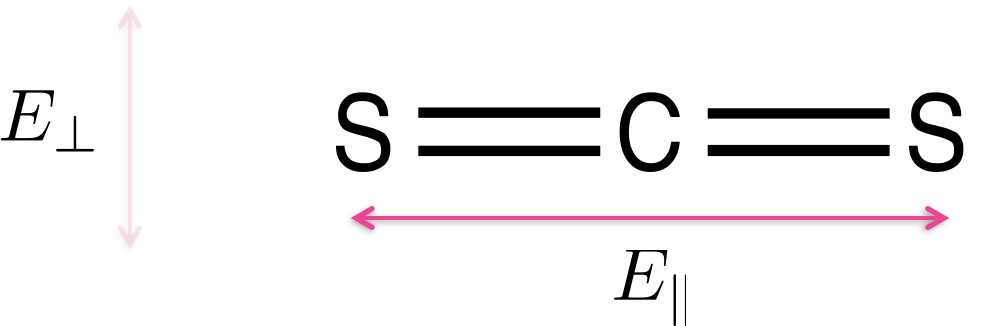
\includegraphics[width=0.6\linewidth]{images/CS2} 

}

\caption{Carbon disulfide (CS~2~) is a linear molecule -  due to the shape of the molecule there is a transition dipole which runs down the length of the long axis. Light aligned such that the electric field runs parallel with the long axis of the molecule E~||~ will be absorbed, light which in which the electric field runs perpendicular to the long axis of the molecule E~⊥~ will not be absorbed.}\label{fig:CS2}
\end{figure}

For more complicated molecules each of the transitions from the HOMO, HOMO-1 to the LUMO \emph{etc.} occur with different transition dipole moments across the chromophore, figure @ref\{fig:adenosine\}. Each transition is only excited when light is aligned with that transition; in most cases this isn't something we need to consider as most incident light we consider is isotropic, but alignment of transition dipoles (either between light and molecules - or between two different molecules) is an important consideration.

\begin{figure}

{\centering 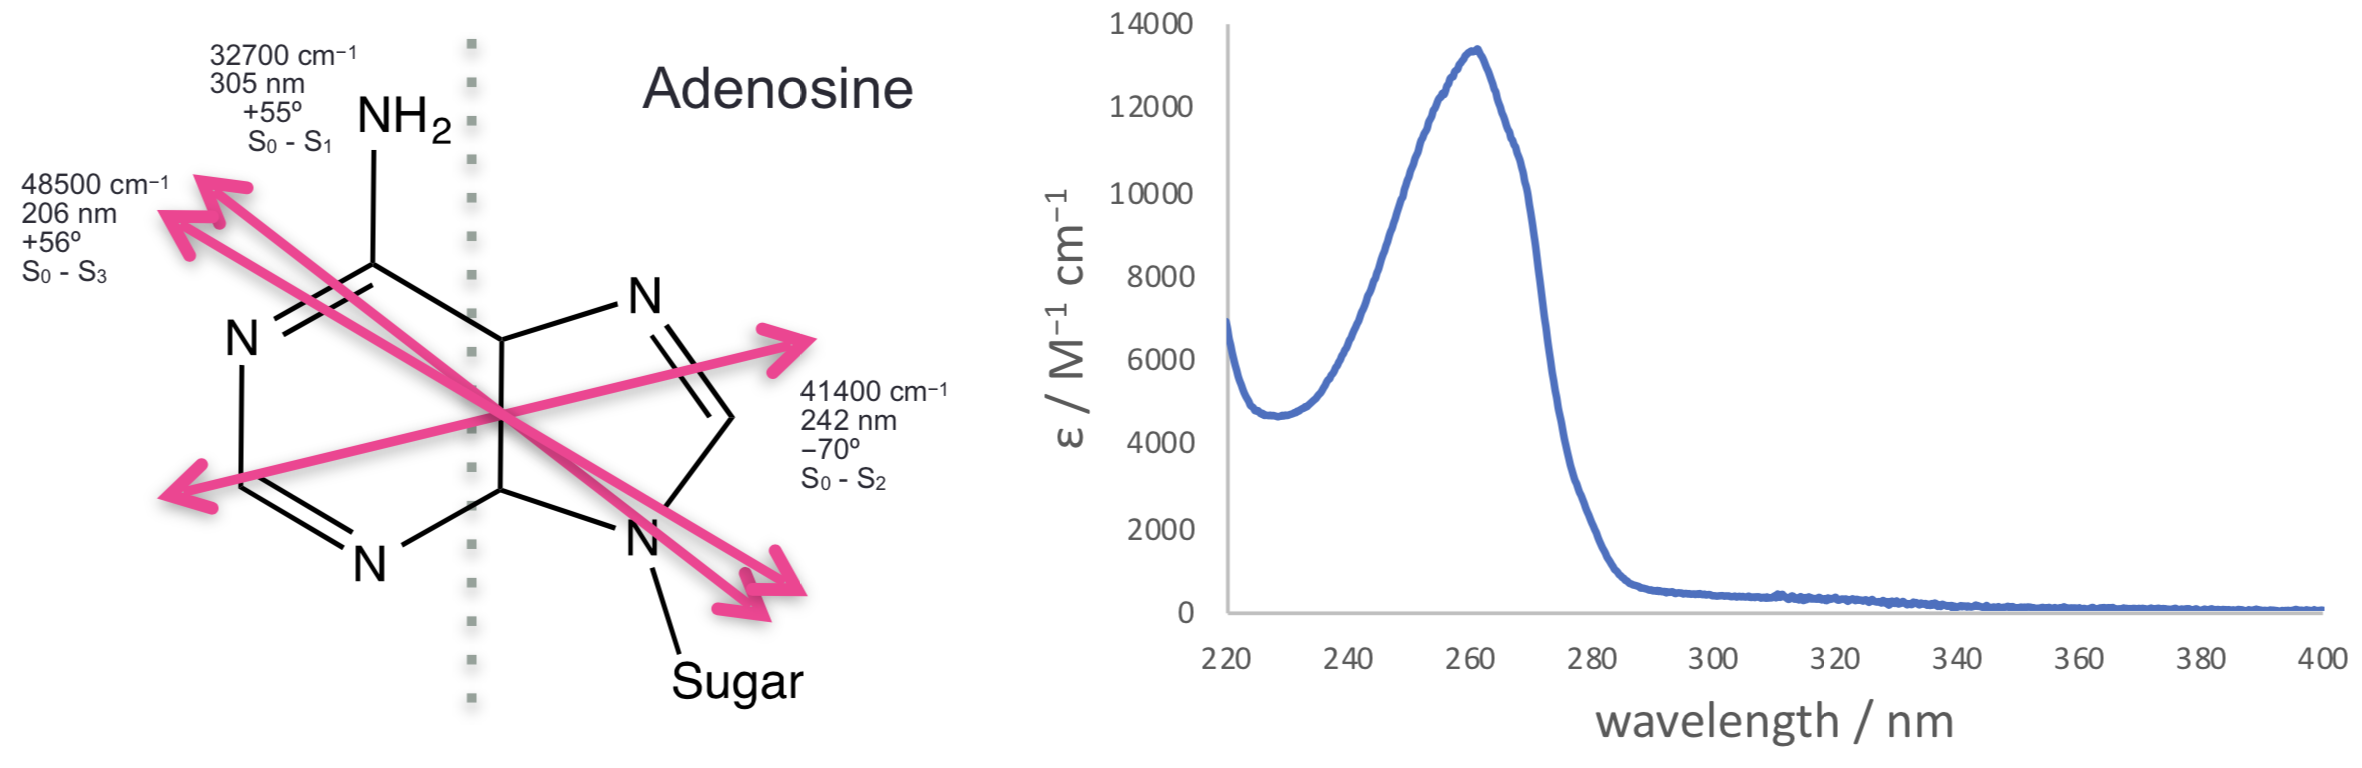
\includegraphics[width=1\linewidth]{images/adenosine} 

}

\caption{The three lowest energy transitions of adenosine each indicated with their transition dipole moment (all in the plane of the molecule, calculated values).These match with the observed spectrum with a weak transition around 310 nm, a much stronger transition around 260 nm and a third transition starting at the edge of the measured spectrum. [Spectrum [Adapted from OMLC]( https:// omlc.org/spectra/PhotochemCAD/html/033.html), 31st October 2018]}\label{fig:adenosine}
\end{figure}

As already discussed the transition dipole moment is derived from the difference in electron density of the ground and excited state. Figure \ref{fig:PhenRubpy3} shows the HOMO and LUMO of an organic chromophore, and a metal complex MLCT state.

\begin{figure}

{\centering 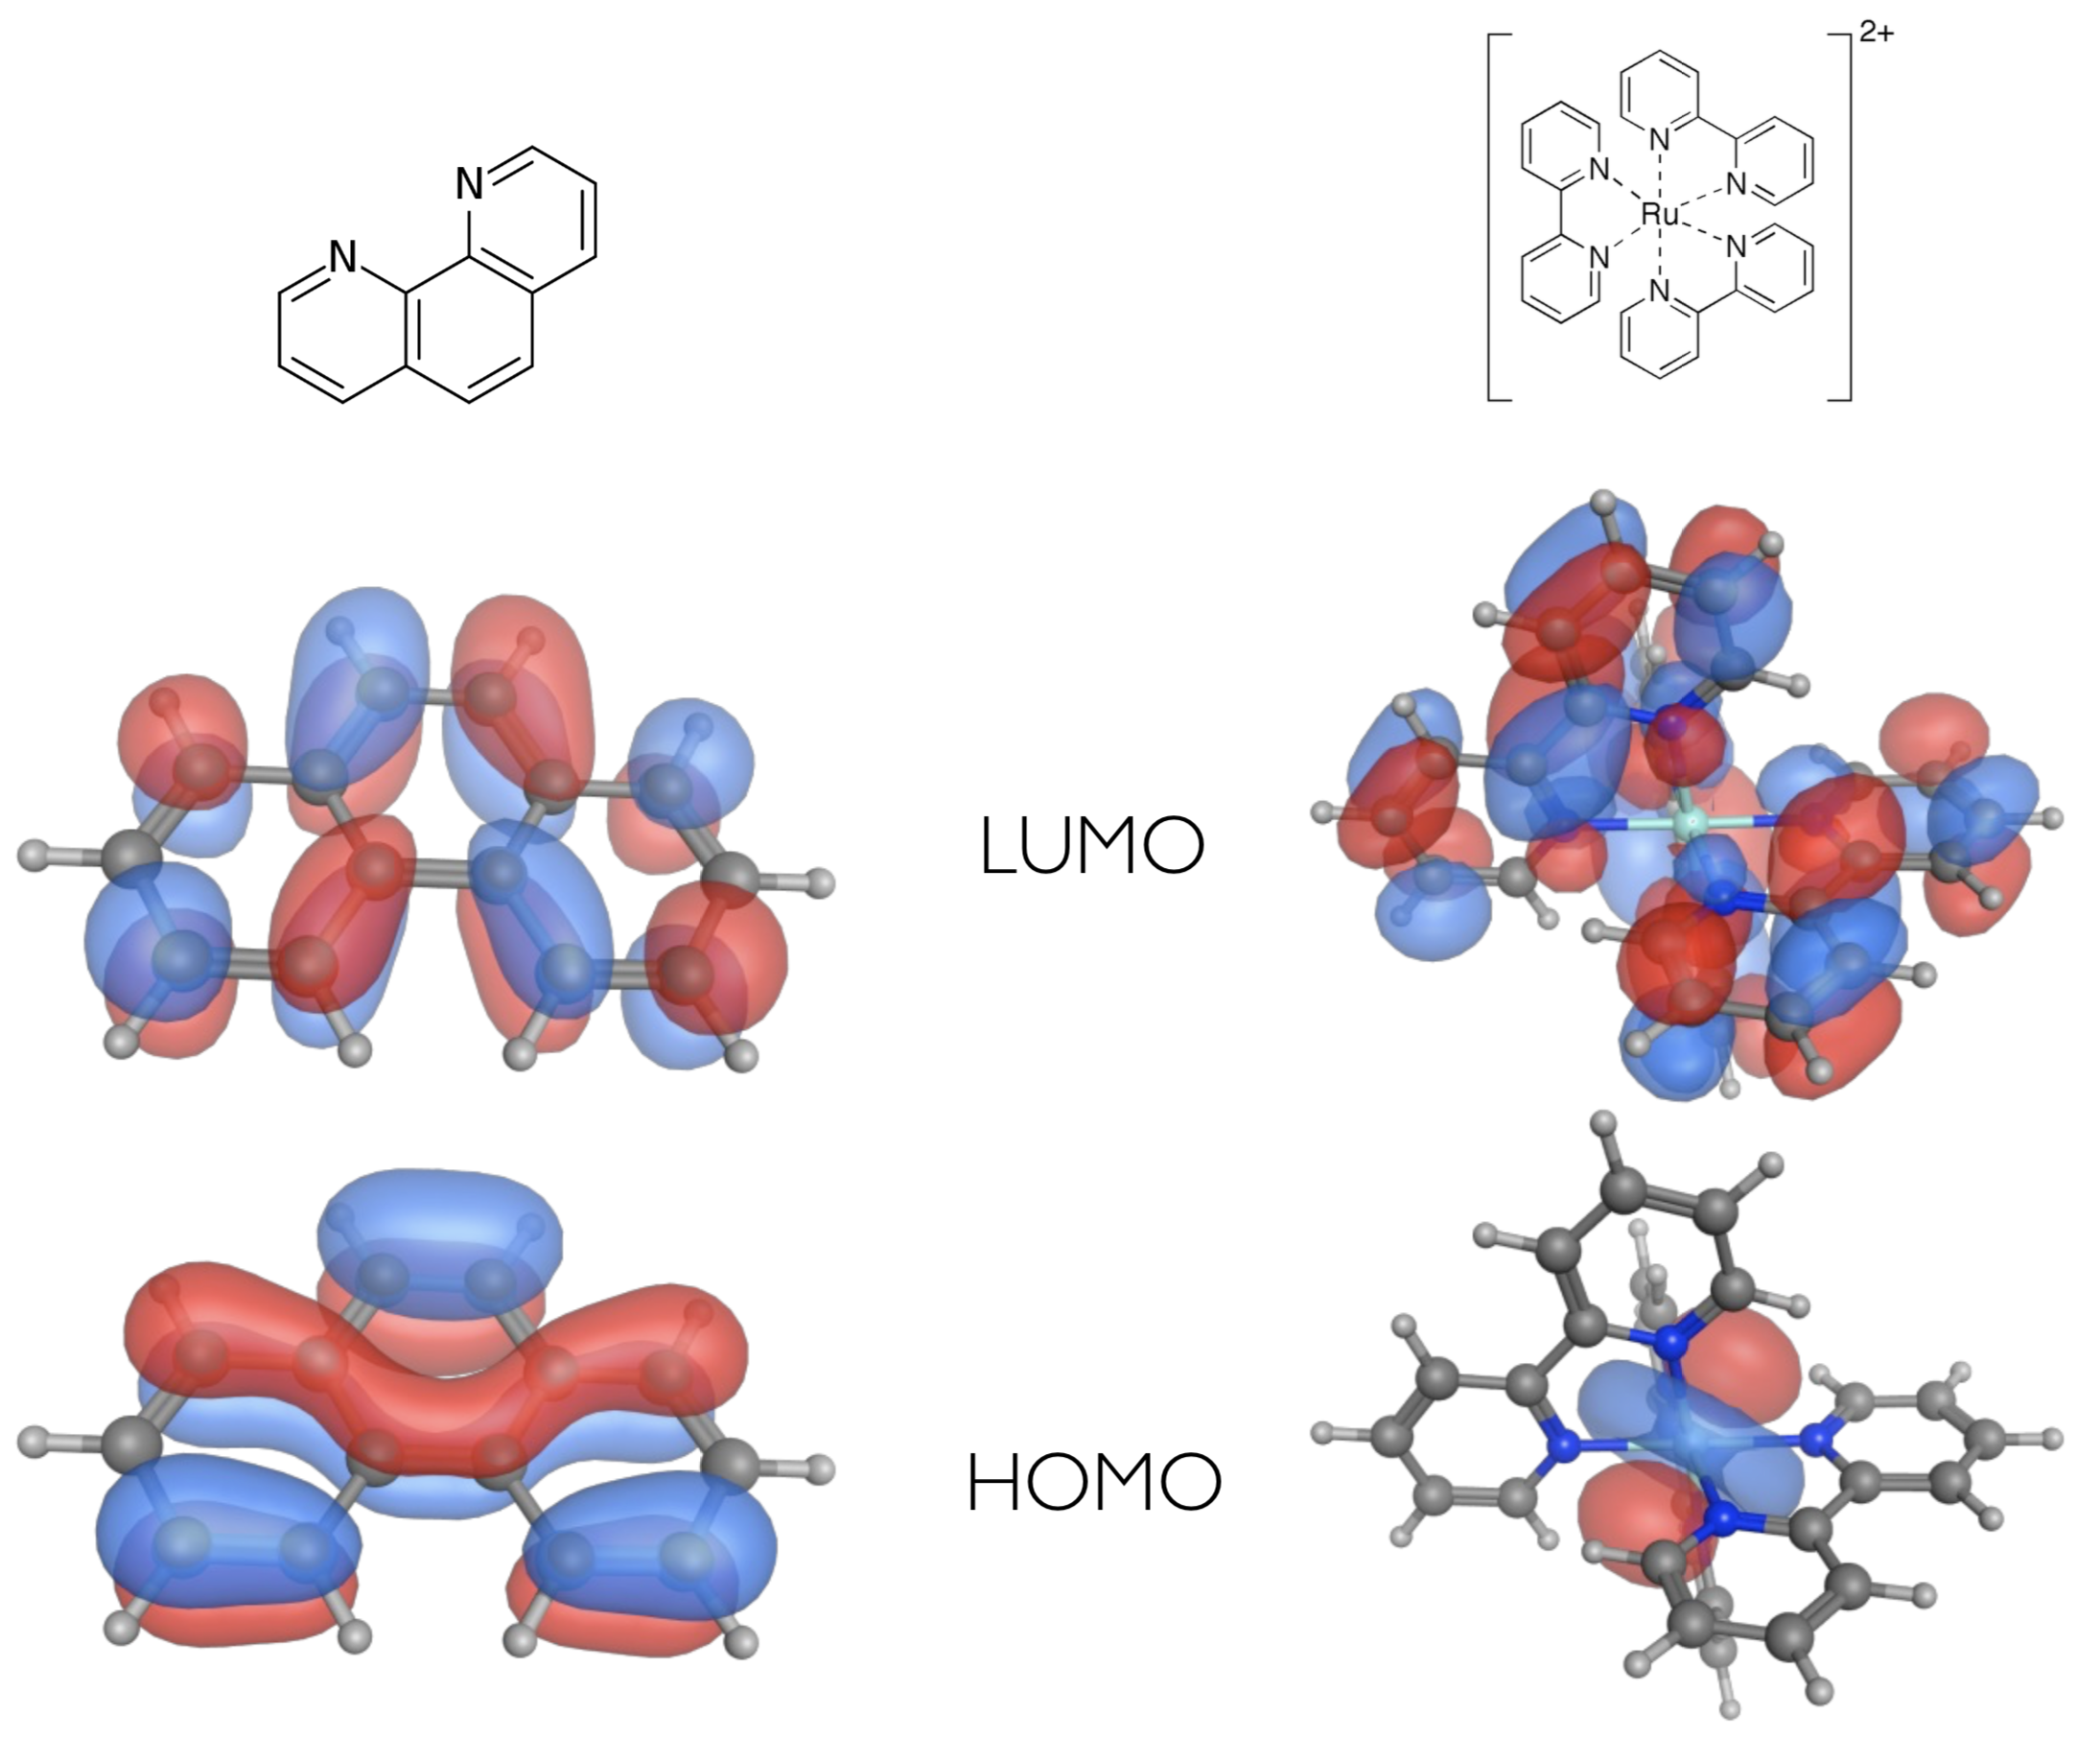
\includegraphics[width=1\linewidth]{images/PhenRubpy3} 

}

\caption{The calculated HOMO (bottom) and LUMO (top) of 1,10-phenanthroline (left) a model planar organic chromophore and [Ru (bpy)$_3$]$^{2+}$ (bpy - bipyridine) which has an MLCT state. For the ruthenium complex the HOMO is clearly centred on $4d_{z^2}$ orbital, whereas after absorption of a photon (and transfer of the electron) the electron density is then centred over the ligands in the LUMO.}\label{fig:PhenRubpy3}
\end{figure}

\hypertarget{factors-which-affect-the-absorption}{%
\section{Factors Which Affect the Absorption}\label{factors-which-affect-the-absorption}}

In the condensed phase the solvent is an important factor in determining the wavelength of maximum absorption, this effect, called solvatochromism, can be due to many properties of the solvent but is most likely due to solvent polarity. The LUMO energy level is unchanged in the different solvents, but the HOMO can either be more stabilised or less stabilised by the change in solvent (Figure \ref{fig:solvato}).

\begin{figure}

{\centering 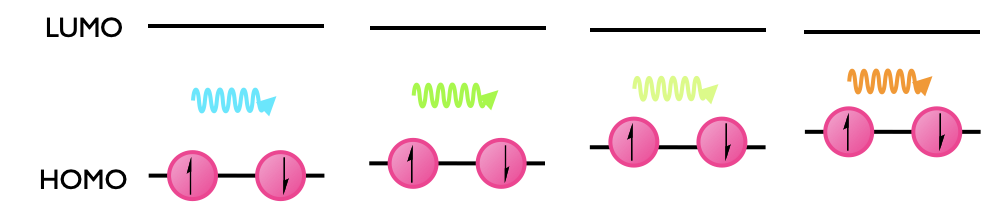
\includegraphics[width=1\linewidth]{images/Solvatochromism} 

}

\caption{The change in absorption wavelength as the HOMO is destabilised in a solvent series, here is worth noting that the colour observed and the wavelength of maximum absorption are not the same thing. As the HOMO is destabilised there is a red shift in the wavelength required to excite the electron.}\label{fig:solvato}
\end{figure}

This leads to a change in the HOMO LUMO energy gap and consequently a change in the wavelength of maximum absorption.

If the absorption maxima shifts to increasing wavelength (red shift, decreasing energy of transition) it is referred to as a bathochromic shift, whereas if the absorption maxima shifts to decreasing wavelength (blue shift, increasing energy of transition) it is referred to as a hypsochromic shift.

Another major factor that can affect the absorption of a sample are interactions between the chromophores. This is most commonly encountered with DNA, which shows a significantly higher absorption at high temperatures (Figure \ref{fig:DNAmelt}). This is because the bases of DNA `stack' to form the rungs of a ladder, this stacking has favourable \(\pi - \pi\) interactions which help to stabilise the macromolecule. As the DNA is heated the double helix begins to melt and the rigid ladder stack is broken. The favourable \(\pi - \pi\) interactions are lost and so the absorption increases. There is little or no change in the wavelength of the maximum absorbance in this process only an increase in the absorbance due to a higher value of molar extinction coefficient. This effect as the absorbance of DNA increases upon melting is called hyperchromicity, the converse, a decrease in absorption, is called hypochromicity.

\begin{figure}

{\centering 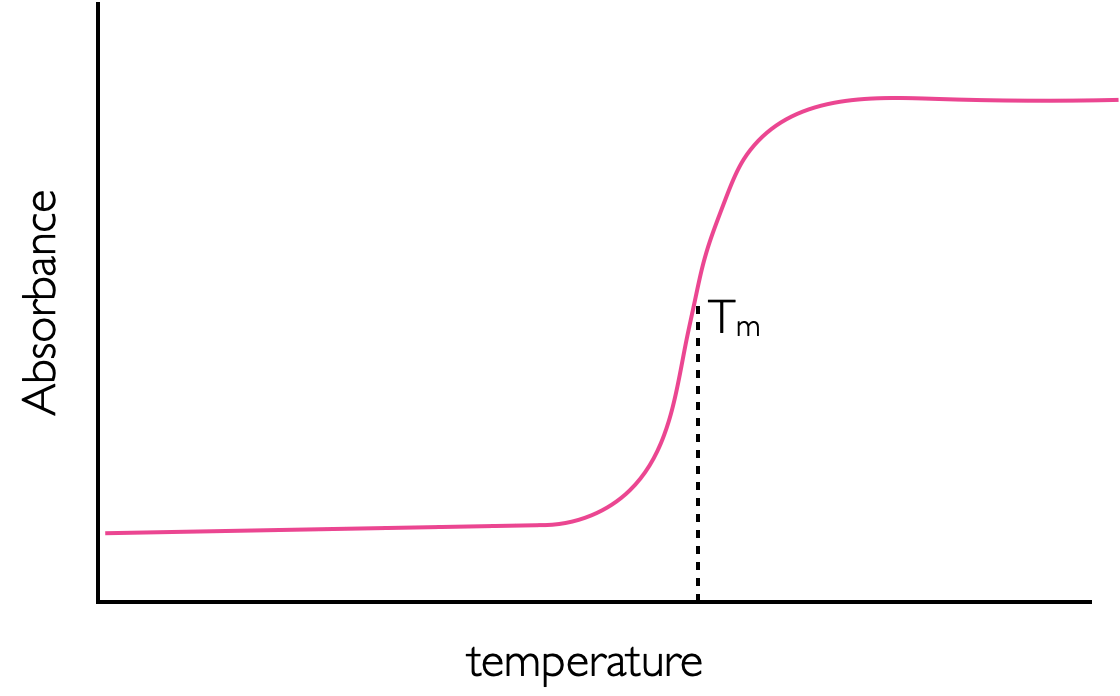
\includegraphics[width=0.6\linewidth]{images/DNAmelt} 

}

\caption{A sketch of the melting of DNA leading to a large increase in absorption. The melting temperature T~m~, is defined much as the end point of a titration curve is, as halfway between the two turning points. The increase in absorbance is due to the breaking of the π stack which exists in double stranded helical DNA.}\label{fig:DNAmelt}
\end{figure}

\hypertarget{sec:before1}{%
\section{Before Completing this Section}\label{sec:before1}}

To support the material in this section it is suggested you read chapter 2 of Wardle `Principles and Application of Photochemistry' and the section in Atkins' `Physical Chemistry' on Einstein coefficients. If you need a refresher of some MO theory it is recommended you look at the early chapters of Chemistry\textsuperscript{3}.

\hypertarget{ch:Workshop1}{%
\chapter{Workshop Questions for Week 2 Absorption}\label{ch:Workshop1}}

\hypertarget{sec:BeerLambertSAQ}{%
\section{Short mathematical question - Beer Lambert law}\label{sec:BeerLambertSAQ}}

\begin{itemize}
\tightlist
\item
  How far can monochromatic 489 nm light travel through a 0.100 M solution of fluorescein with an extinction coefficient at 489 nm of 92000 M\textsuperscript{−1} cm\textsuperscript{−1} before 90 \% of it is absorbed?
\end{itemize}

\emph{(I will use MCQs and UniDoodle to ask this in class)}

\hypertarget{sec:MolarExtinction}{%
\section{Short conceptual question - molar extinction coefficient}\label{sec:MolarExtinction}}

\begin{itemize}
\tightlist
\item
  Modify the molecule in figure \ref{fig:bpy1} to increase the molar extinction coefficient (do not worry about what may happen to wavelength).
\end{itemize}

\begin{figure}

{\centering 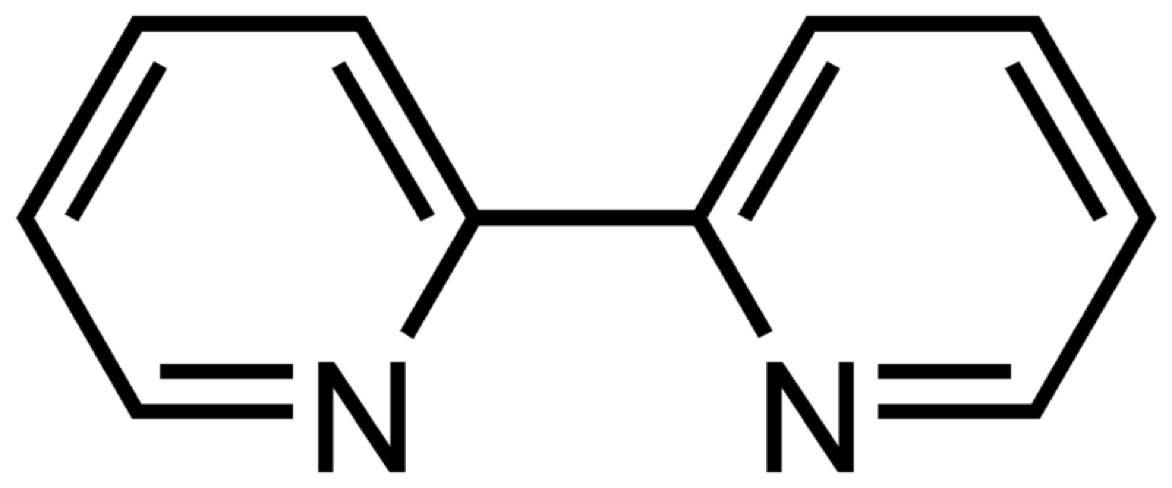
\includegraphics[width=0.3\linewidth]{images/bpy} 

}

\caption{The structure of bipyridine (also known as bpy).}\label{fig:bpy1}
\end{figure}

\emph{(I will use UniDoodle's drawing feature to ask this in class)}

\hypertarget{sec:intensity}{%
\section{Short conceptual question - intensity of colour}\label{sec:intensity}}

\begin{itemize}
\tightlist
\item
  What factors influence the `intensity of colour' of the following solutions?
\end{itemize}

\begin{figure}

{\centering 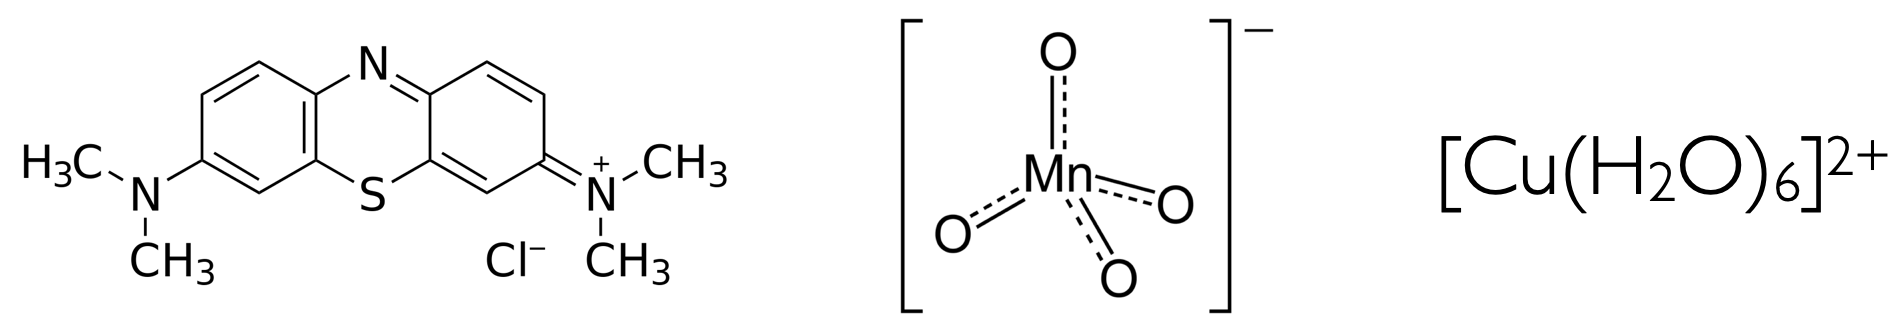
\includegraphics[width=0.7\linewidth]{images/molarextquestion} 

}

\caption{The structures of the organic dye methylene blue (left), potassium permanganate (centre) and copper hexa-aqua (right).}\label{fig:molarextstructures1}
\end{figure}

\begin{figure}

{\centering 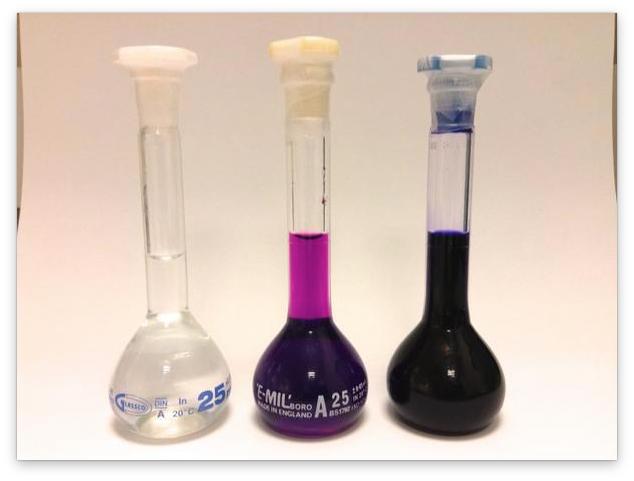
\includegraphics[width=0.7\linewidth]{images/Molar_extinction_coefficients} 

}

\caption{1 mM solutions of the organic dye methylene blue (right), potassium permanganate (centre) and copper hexa-aqua (left).}\label{fig:molarextsolutions1}
\end{figure}

\emph{(This will be a discussion question)}

\hypertarget{sec:linewidth}{%
\section{Short conceptual question - line width}\label{sec:linewidth}}

\begin{itemize}
\tightlist
\item
  Why are some spectra very broad (figure \ref{fig:rhodaminemol}), whereas others have sharp peaks (figure \ref{fig:atomictin})?
\end{itemize}

You will need to look at the x-scale to truley note the difference in the width of these emission spectra.

\begin{figure}

{\centering 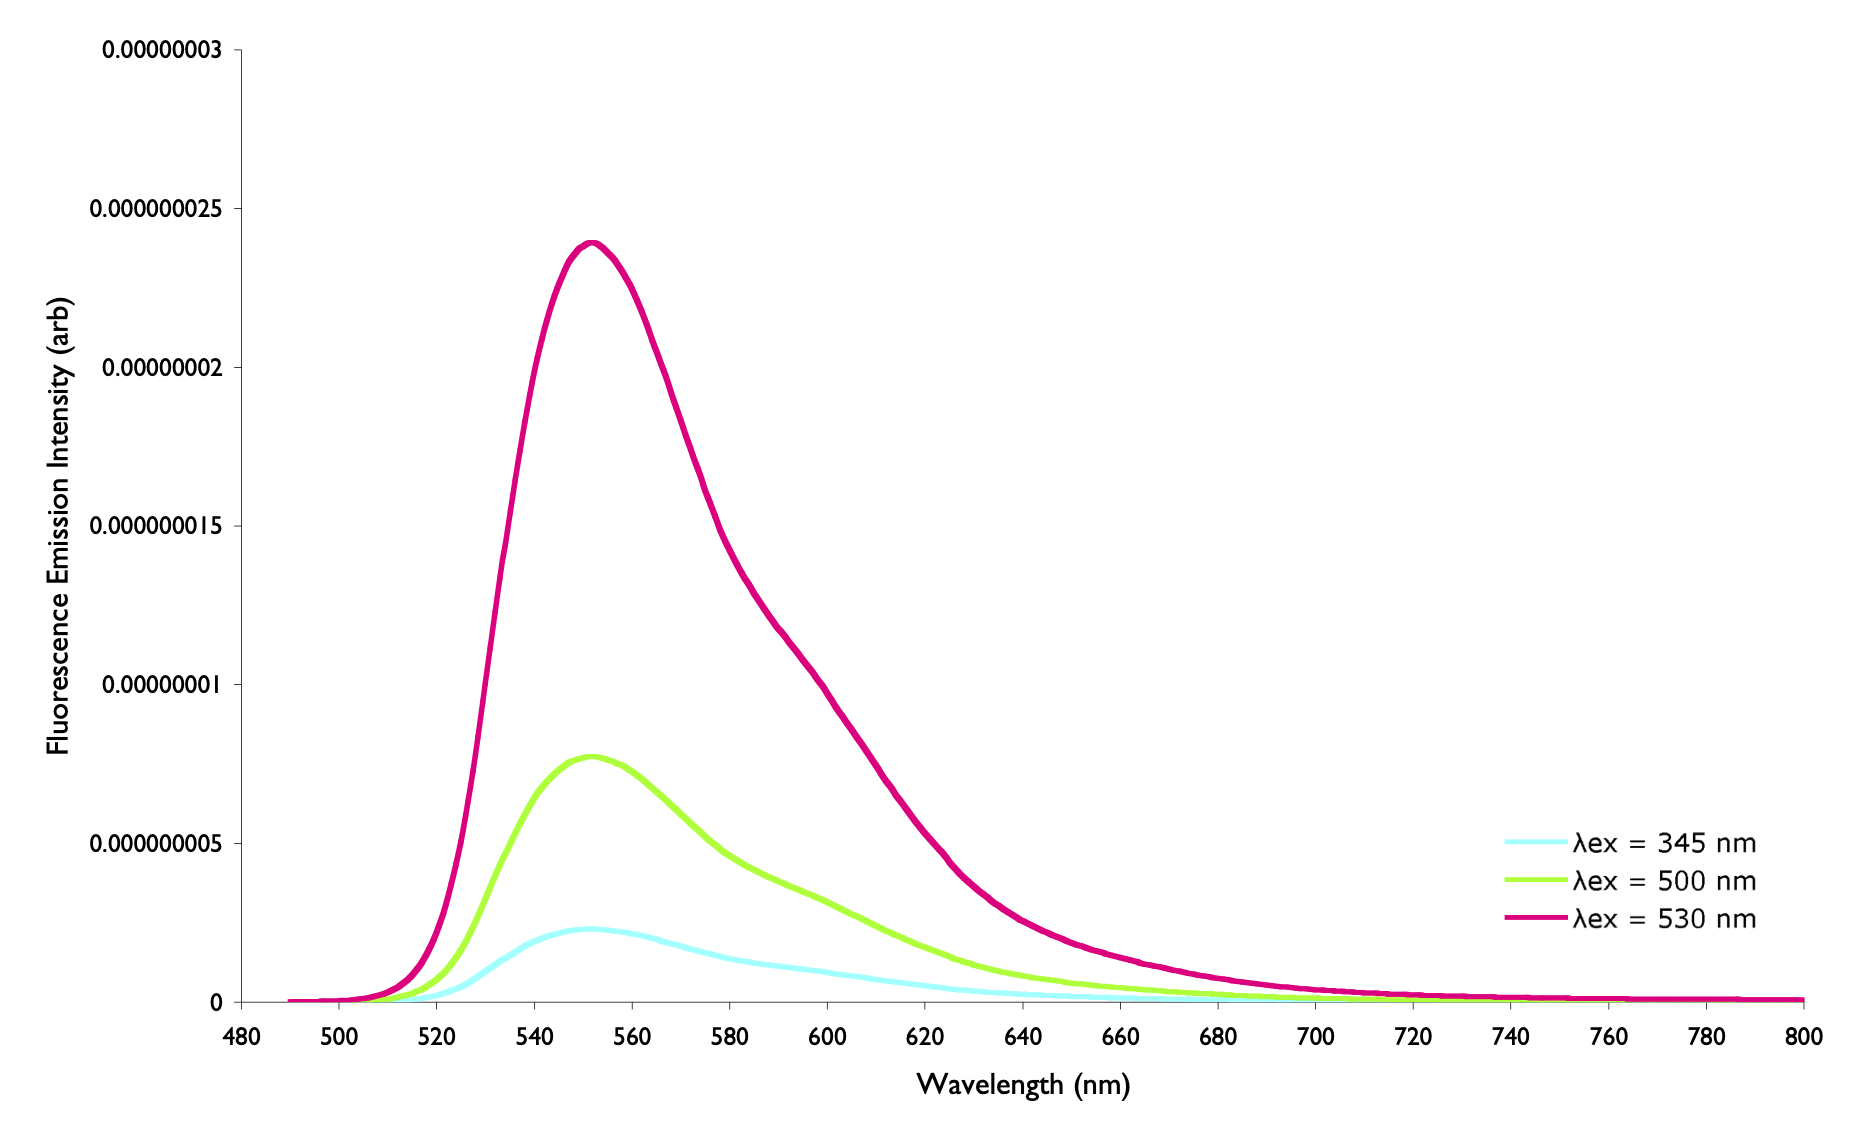
\includegraphics[width=0.7\linewidth]{images/rhodamine6G} 

}

\caption{The emission spectrum of rhodamine 6G}\label{fig:rhodaminemol}
\end{figure}

\begin{figure}

{\centering 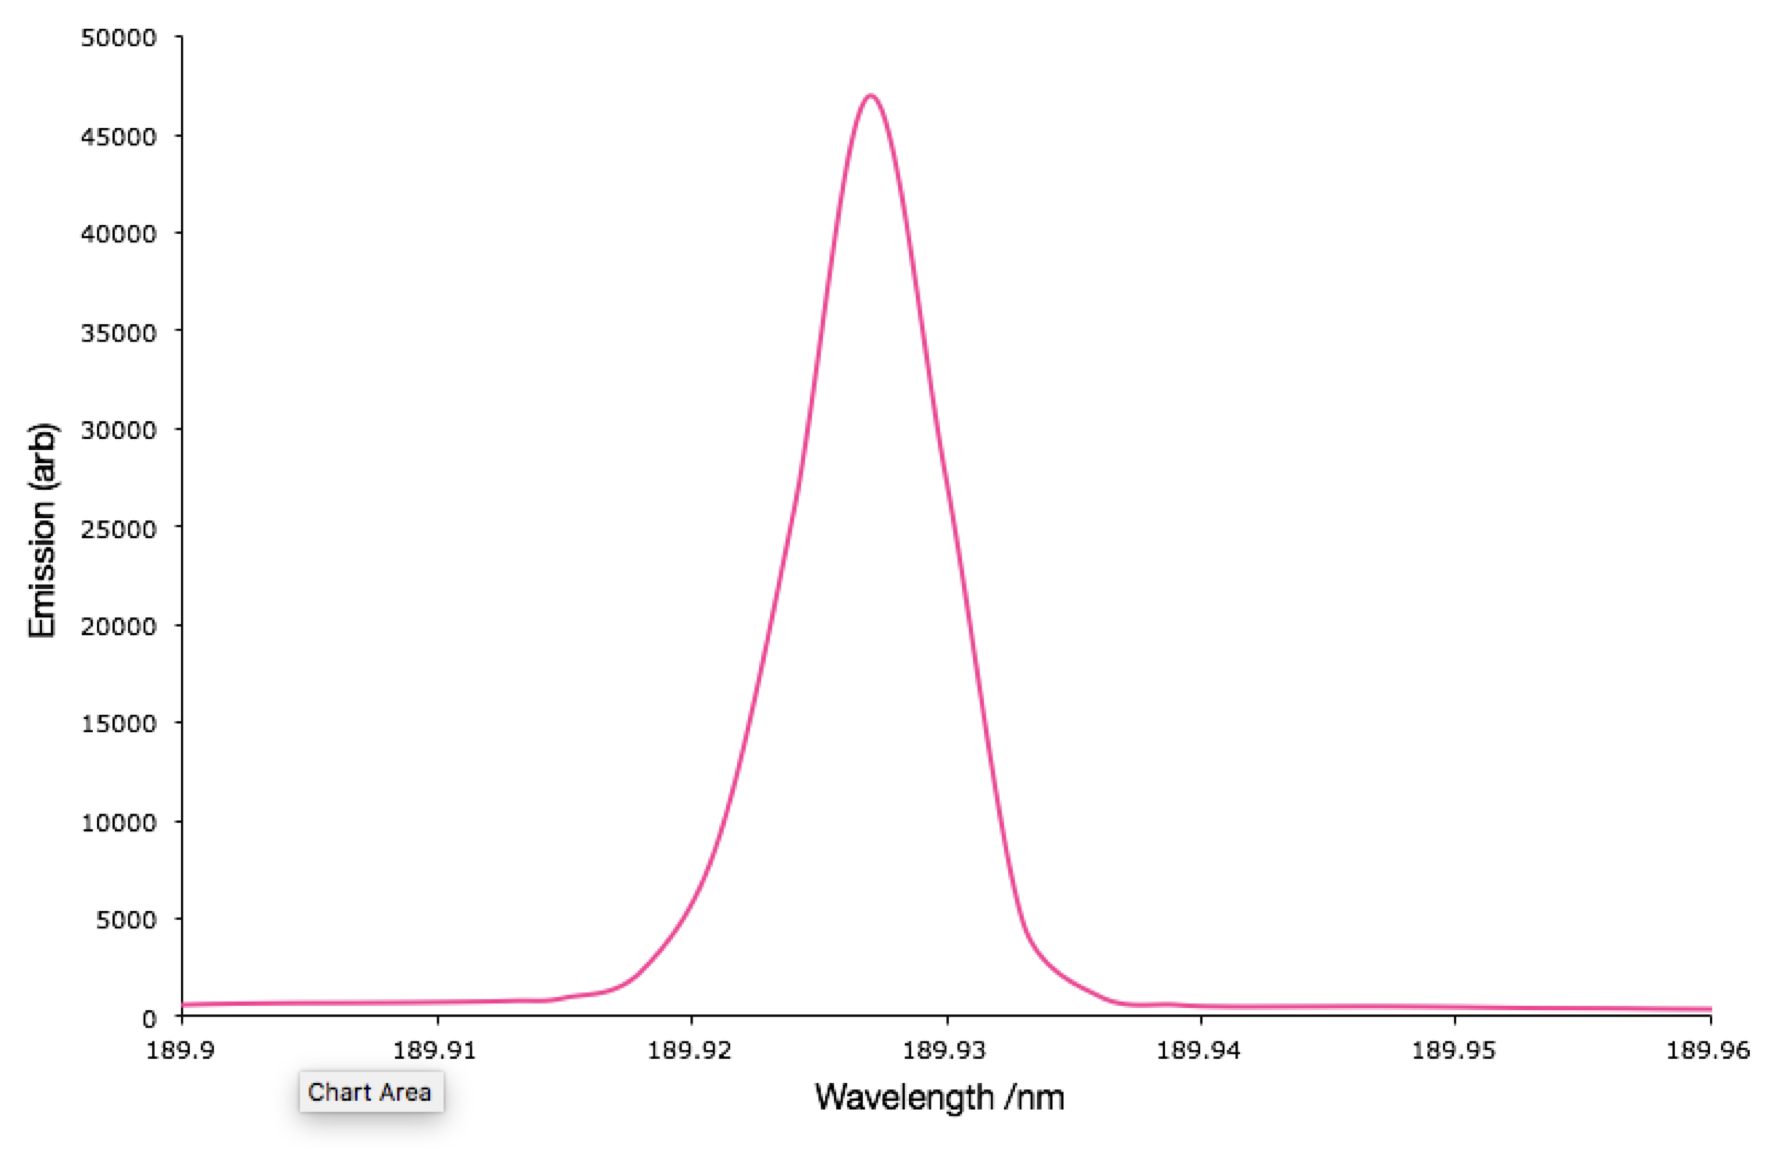
\includegraphics[width=0.7\linewidth]{images/atomic_emission_spectrum} 

}

\caption{The emission spectrum of Sn(II)}\label{fig:atomictin}
\end{figure}

\emph{(This will be a discussion question)}

\hypertarget{sec:solvationabs}{%
\section{Short conceptual question - the effect of solvation on absorbance}\label{sec:solvationabs}}

\begin{figure}

{\centering 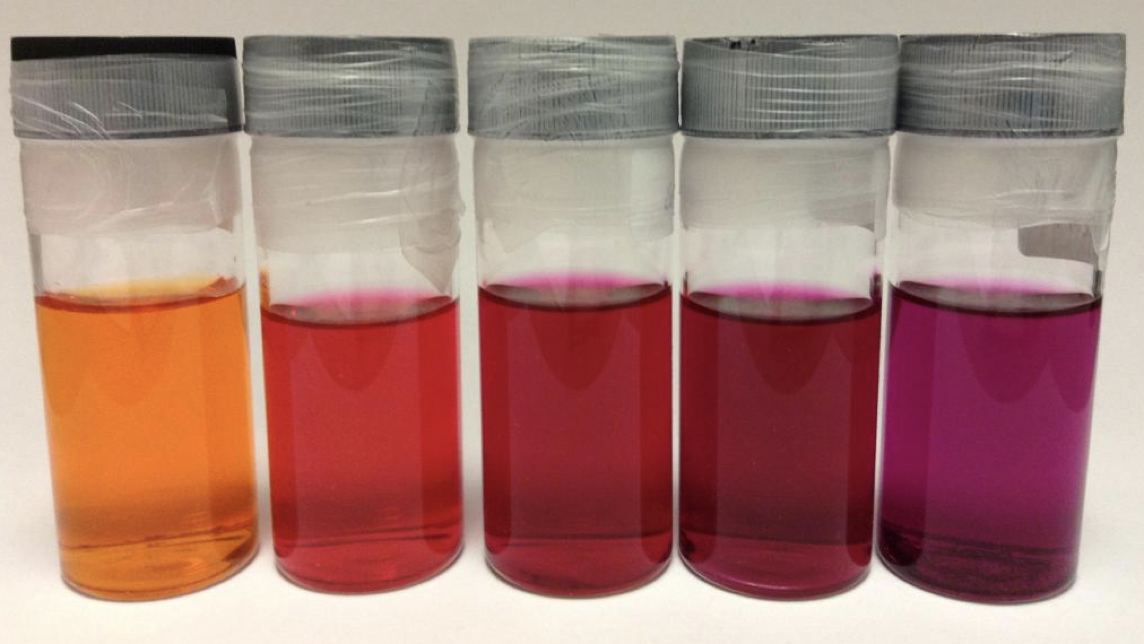
\includegraphics[width=0.7\linewidth]{images/ethidium} 

}

\caption{Ethidium bromide dissolved in from right; water(orange), methanol, ethanol, propanol and butanol(purple)}\label{fig:ethidiumsolvent}
\end{figure}

\begin{itemize}
\tightlist
\item
  Why does the observed colour of ethidium bromide depend upon the solvent (figure \ref{fig:ethidiumsolvent}))?
\end{itemize}

Think about the effect of solvation on the energy levels and why those energy levels matter! Remember that if light is transmitted through a solution that is the colour we observe\ldots{}

\emph{(This will be a discussion question)}

\hypertarget{sec:Azobenzene}{%
\section{Extended question - Azobenzene}\label{sec:Azobenzene}}

Azobenzene undergoes the following cis-trans isomerisation, the isomerisation occurs in the ps timescale.

\begin{figure}

{\centering 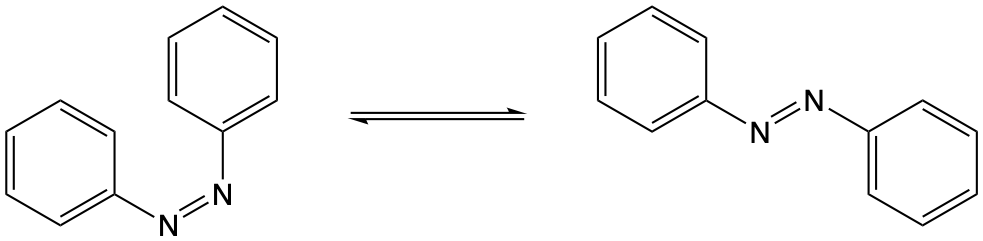
\includegraphics[width=0.7\linewidth]{images/cistransazobenzene} 

}

\caption{The cis-trans isomerisation of azobenzene}\label{fig:cistransazobenzeneisomerisation}
\end{figure}

\begin{itemize}
\item
  Why would you expect the absorption spectrum of each isomer to be different?
\item
  Suggest why the trans conformation is more stable than the cis isomer.
\item
  Use the following data to predict the proportion of each isomer under 360 nm excitation.
\end{itemize}

\begin{longtable}[]{@{}lll@{}}
\caption{\label{tab:azobenzeneabs} The molar extinction coefficient of the two isomers of azobenzene.}\tabularnewline
\toprule
& ε\textsubscript{360} / M\textsuperscript{−1} cm\textsuperscript{−1} & ε\textsubscript{460} / M\textsuperscript{−1} cm\textsuperscript{−1}\tabularnewline
\midrule
\endfirsthead
\toprule
& ε\textsubscript{360} / M\textsuperscript{−1} cm\textsuperscript{−1} & ε\textsubscript{460} / M\textsuperscript{−1} cm\textsuperscript{−1}\tabularnewline
\midrule
\endhead
trans-azobenzene & 22000 & 4500\tabularnewline
cis-azobenzene & 2100 & 5500\tabularnewline
\bottomrule
\end{longtable}

\begin{itemize}
\item
  Would there be more or less trans azobenzene at 460 nm? Justify your answer.
\item
  It has been suggested the 360 nm absorption is an S\textsubscript{0} → S\textsubscript{2} absorption, and the 460 nm band is an S\textsubscript{0} → S\textsubscript{1} absorption. Suggest which energy levels are involved for each of the two transitions and compare it to stilbene which has a similar structure, but the cis and trans absorptions are 280 \& 295 nm respectively.
\end{itemize}

\begin{figure}

{\centering 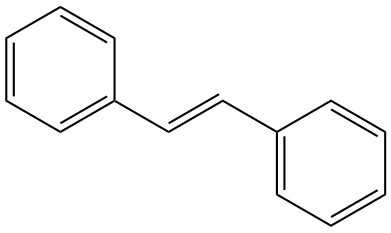
\includegraphics[width=0.3\linewidth]{images/stilbene} 

}

\caption{The  structure of stilbene}\label{fig:stilbene}
\end{figure}

\emph{(This will be a discussion question)}

\hypertarget{ch:Em}{%
\chapter{Emission of Light}\label{ch:Em}}

\hypertarget{sec:EmLOs}{%
\subsection{Learning Objectives}\label{sec:EmLOs}}

At the end of this block you should be able to:

\begin{itemize}
\item
  Define singlet and triplet states in terms of molecular orbitals
\item
  Explain the mirror symmetry observed in absorption/fluorescence spectra.
\item
  Construct and explain the Jablonski diagram.
\item
  Define the rates of the processes in the Jablonski scheme and give typical values for the rate constants.
\item
  Define singlet and triplet lifetimes and describe how they are measured.
\item
  Analyse decay curves to obtain lifetimes of excited states.
\item
  Define and derive the quantum yield of fluorescence and phosphorescence.
\end{itemize}

Only the light absorbed by a molecule can produce photochemical change in a molecule. If a species absorbs radiation then one particle is excited for each quantum of radiation absorbed. This concept of light having to be absorbed before anything else can happen is an obvious one, but is an important concept in itself, it goes on to define the concept of quantum yield of a process, effectively the proportion of excited states which `decay' to any given pathway.

\hypertarget{sec:FluorPhos}{%
\section{Fluorescence \& Phosphorescence}\label{sec:FluorPhos}}

Just as there are `spin forbidden' and `spin allowed' processes for absorption, when the molecule is in an excited state there are a allowed and forbidden path ways of deactivation of the excited state.

If we look at a Jablonski diagram, figure 19, which you should already be familiar with, it shows the range of photophysical deactivation pathways of an excited state.

A Jablonski diagram (figure \ref{fig:Jablonski}) usually uses a short hand to refer to the excited states, where a ground state, if it is a singlet, is referred to as S\textsubscript{0}, and each subsequent excited state is referred to as S\textsubscript{1}, S\textsubscript{2} \emph{etc}.

\begin{figure}

{\centering 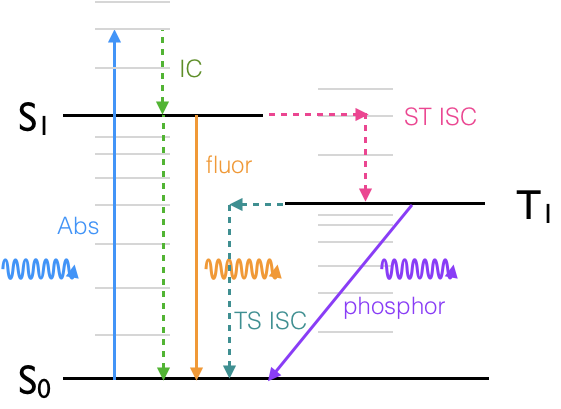
\includegraphics[width=0.7\linewidth]{images/Jablonski} 

}

\caption{Jablonski diagram showing: A, the absorption of a photon, and the photophysical deactivation pathways, IC, internal conversion, ISC, intersystem crossing, F, fluorescence \& P, phosphorescence.}\label{fig:Jablonski}
\end{figure}

Triplet states are referred to as T\textsubscript{1}, T\textsubscript{2}\ldots{} if the ground state is not a triplet then there is no state labelled T\textsubscript{0}. All excited states are referred to by integer vales of 1 or more.

\emph{A note on Jablonski diagrams: transitions which are either allowed or non-radiative and therefore not governed by selection rules appear as either horizontal or vertical transitions, forbidden transitions (such as phosphorescence) are indicated by transitions which occur at an angle. Radiative transitions (those that occur with either the absorption or emission of a photon) are shown as solid lines with the incident or excident photon shown as a wave like arrow. Non radiative transitions are shown as dashed (or alternatively wiggly) lines to clearly differentiate them from radiative transitions. Transitions with a change of spin are isoenergetic (shown as horizontal lines) before decaying via internal conversion (vertical lines). A Jablonski diagram is a sketch of the energy levels and should not include details of the potential wells of either the ground or excited state.}

The spin selection rule which applies for absorption transitions \(\Delta S = 0\), so formally emission transitions from the S\textsubscript{1} to S\textsubscript{0} are spin allowed, allowed emission transitions are referred to a fluorescence.

Emission transitions that involve a change in spin of the electron, such as from T\textsubscript{1} to S\textsubscript{0}, are spin forbidden, and referred to as phosphorescence. The excited state can also decay via non-radiative transitions and other routes.

Table \ref{tab:phototrans} the deactivation pathways from excited states:

\begin{longtable}[]{@{}lll@{}}
\caption{\label{tab:phototrans} The excitation and decay pathways in molecules.}\tabularnewline
\toprule
\endhead
\begin{minipage}[t]{0.39\columnwidth}\raggedright
\emph{`Allowed transitions'}\strut
\end{minipage} & \begin{minipage}[t]{0.26\columnwidth}\raggedright
\strut
\end{minipage} & \begin{minipage}[t]{0.26\columnwidth}\raggedright
\strut
\end{minipage}\tabularnewline
\begin{minipage}[t]{0.39\columnwidth}\raggedright
Singlet-singlet absorption Singlet-singlet emission\strut
\end{minipage} & \begin{minipage}[t]{0.26\columnwidth}\raggedright
fluorescence\strut
\end{minipage} & \begin{minipage}[t]{0.26\columnwidth}\raggedright
\(S_0 + h \nu \longrightarrow S_1\) \(S_1 \longrightarrow S_0 + h \nu '\)\strut
\end{minipage}\tabularnewline
\begin{minipage}[t]{0.39\columnwidth}\raggedright
\emph{`Forbidden transitions'}\strut
\end{minipage} & \begin{minipage}[t]{0.26\columnwidth}\raggedright
\strut
\end{minipage} & \begin{minipage}[t]{0.26\columnwidth}\raggedright
\strut
\end{minipage}\tabularnewline
\begin{minipage}[t]{0.39\columnwidth}\raggedright
Singlet-triplet absorption Triplet-singlet emission\strut
\end{minipage} & \begin{minipage}[t]{0.26\columnwidth}\raggedright
fluorescence\strut
\end{minipage} & \begin{minipage}[t]{0.26\columnwidth}\raggedright
\(S_0 + h \nu \longrightarrow T_1\) \(T_1 \longrightarrow S_0 + h \nu ''\)\strut
\end{minipage}\tabularnewline
\begin{minipage}[t]{0.39\columnwidth}\raggedright
\emph{`Other transitions'}\strut
\end{minipage} & \begin{minipage}[t]{0.26\columnwidth}\raggedright
\strut
\end{minipage} & \begin{minipage}[t]{0.26\columnwidth}\raggedright
\strut
\end{minipage}\tabularnewline
\begin{minipage}[t]{0.39\columnwidth}\raggedright
Internal conversion \strut
\end{minipage} & \begin{minipage}[t]{0.26\columnwidth}\raggedright
(vibrational relaxation) (vibrational relaxation)\strut
\end{minipage} & \begin{minipage}[t]{0.26\columnwidth}\raggedright
\(S_1 \longrightarrow S_0 + heat\) \(S_1 \longrightarrow T_1 + heat\) \(T_1 \longrightarrow S_0 + heat\)\strut
\end{minipage}\tabularnewline
\begin{minipage}[t]{0.39\columnwidth}\raggedright
\emph{Other pathways}\strut
\end{minipage} & \begin{minipage}[t]{0.26\columnwidth}\raggedright
\strut
\end{minipage} & \begin{minipage}[t]{0.26\columnwidth}\raggedright
\strut
\end{minipage}\tabularnewline
\begin{minipage}[t]{0.39\columnwidth}\raggedright
Quenching of excited state Chemistry from excited state\strut
\end{minipage} & \begin{minipage}[t]{0.26\columnwidth}\raggedright
\strut
\end{minipage} & \begin{minipage}[t]{0.26\columnwidth}\raggedright
\(S_1 + Q \longrightarrow S_0 + Q +heat\) \(S_1 + Q \longrightarrow S_0 + Q^\ast +heat\) \(T_1 + Q \longrightarrow S_0 + Q +heat\) \(T_1 + Q \longrightarrow S_0 + Q^\ast +heat\) \(S_1 \longrightarrow\) new/changed molecule\strut
\end{minipage}\tabularnewline
\bottomrule
\end{longtable}

The spin selection rule has important consequences on the lifetime of singlet and triplet states. The spin allowed process of fluorescence usually has a short lifetime (less than 10 ns), whereas the spin forbidden process of phosphorescence has a significantly longer lifetime, which can be as long as several seconds.

Vibrational relaxation occurs in the ps timescale, consequently the excited state decays vibrationally to the S\textsubscript{1}, v' = 0 state and emission essentially always occurs from the ground vibrational electronically excited state. This is an important concept in photophysics and is called Kasha's rule.

\hypertarget{sec:Kasha}{%
\subsection{Kasha's Rule}\label{sec:Kasha}}

\emph{An excited state always emits from the lowest energy level of that spin multiplicity state.}

The Frank-Condon principle applies equally to emission processes and the excited state will decay to a number of available vibrationally excited states of the ground electronic state. After relaxation to the \(v’ = 0\) level emission occurs to each of the available vibrational states of the ground state. The relative intensity of each band depends upon the coupling or overlap integral between the ground and excited states, as shown in figure \ref{fig:anthracenekasha}.

\begin{figure}

{\centering 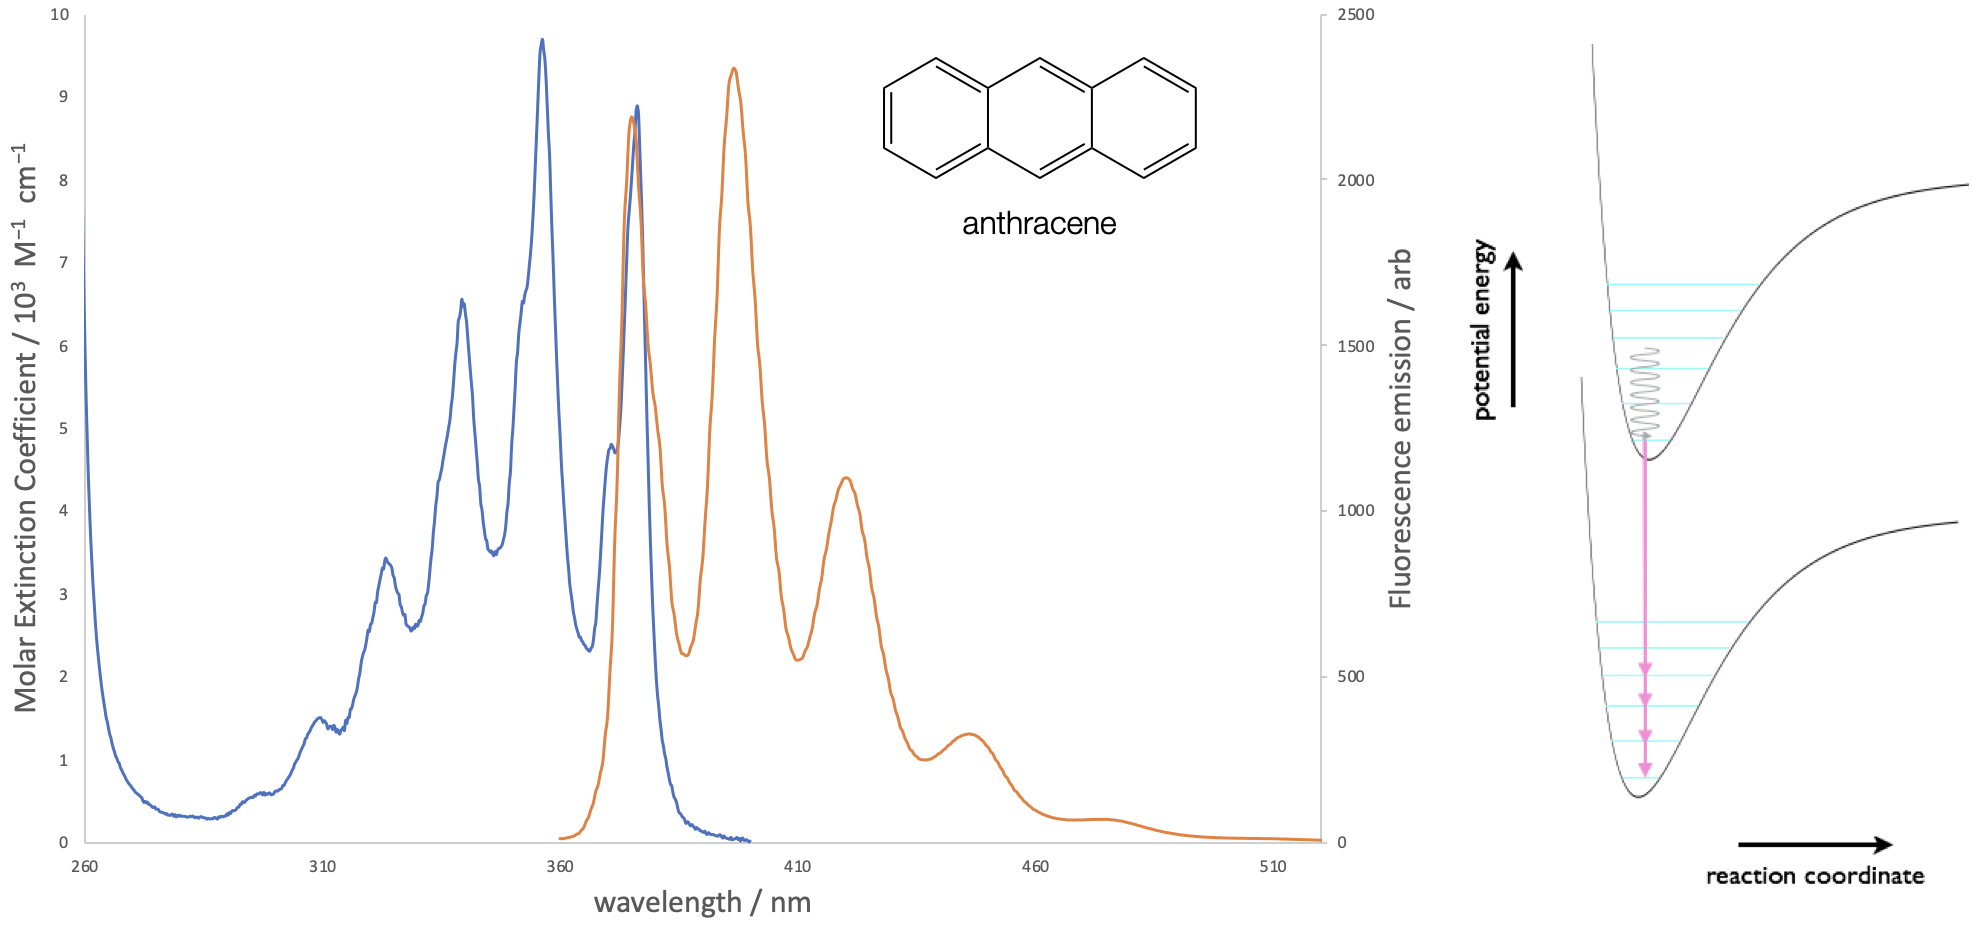
\includegraphics[width=0.7\linewidth]{images/anthracenekasha} 

}

\caption{The absorption and emission spectra of anthracene in ethanol solution. Both the absorption and emission spectra show vibrational fine structure, due to transitions to discrete vibrational energy levels in the excited and ground states respectively.}\label{fig:anthracenekasha}
\end{figure}

\hypertarget{sec:stoke}{%
\section{Stoke's shift}\label{sec:stoke}}

The Franck-Condon factors in absorption and emission is clearly evident by the symmetry shown in the emission of most organic chromophores. The Stoke's shift, the difference between the \(v=0\) to \(v’=0\) absorption peak and the \(v’=0\) to \(v=0\) emission peak, can simply be explained by the offset of the ground and excited state potential wells (figure \ref{fig:stokesspectrum}). Absorption happens from the centre of the \(v=0\) ground state and emission from the centre of the \(v’=0\) excited state, however this does not explain why the two curves are offset from one another.

\begin{figure}

{\centering 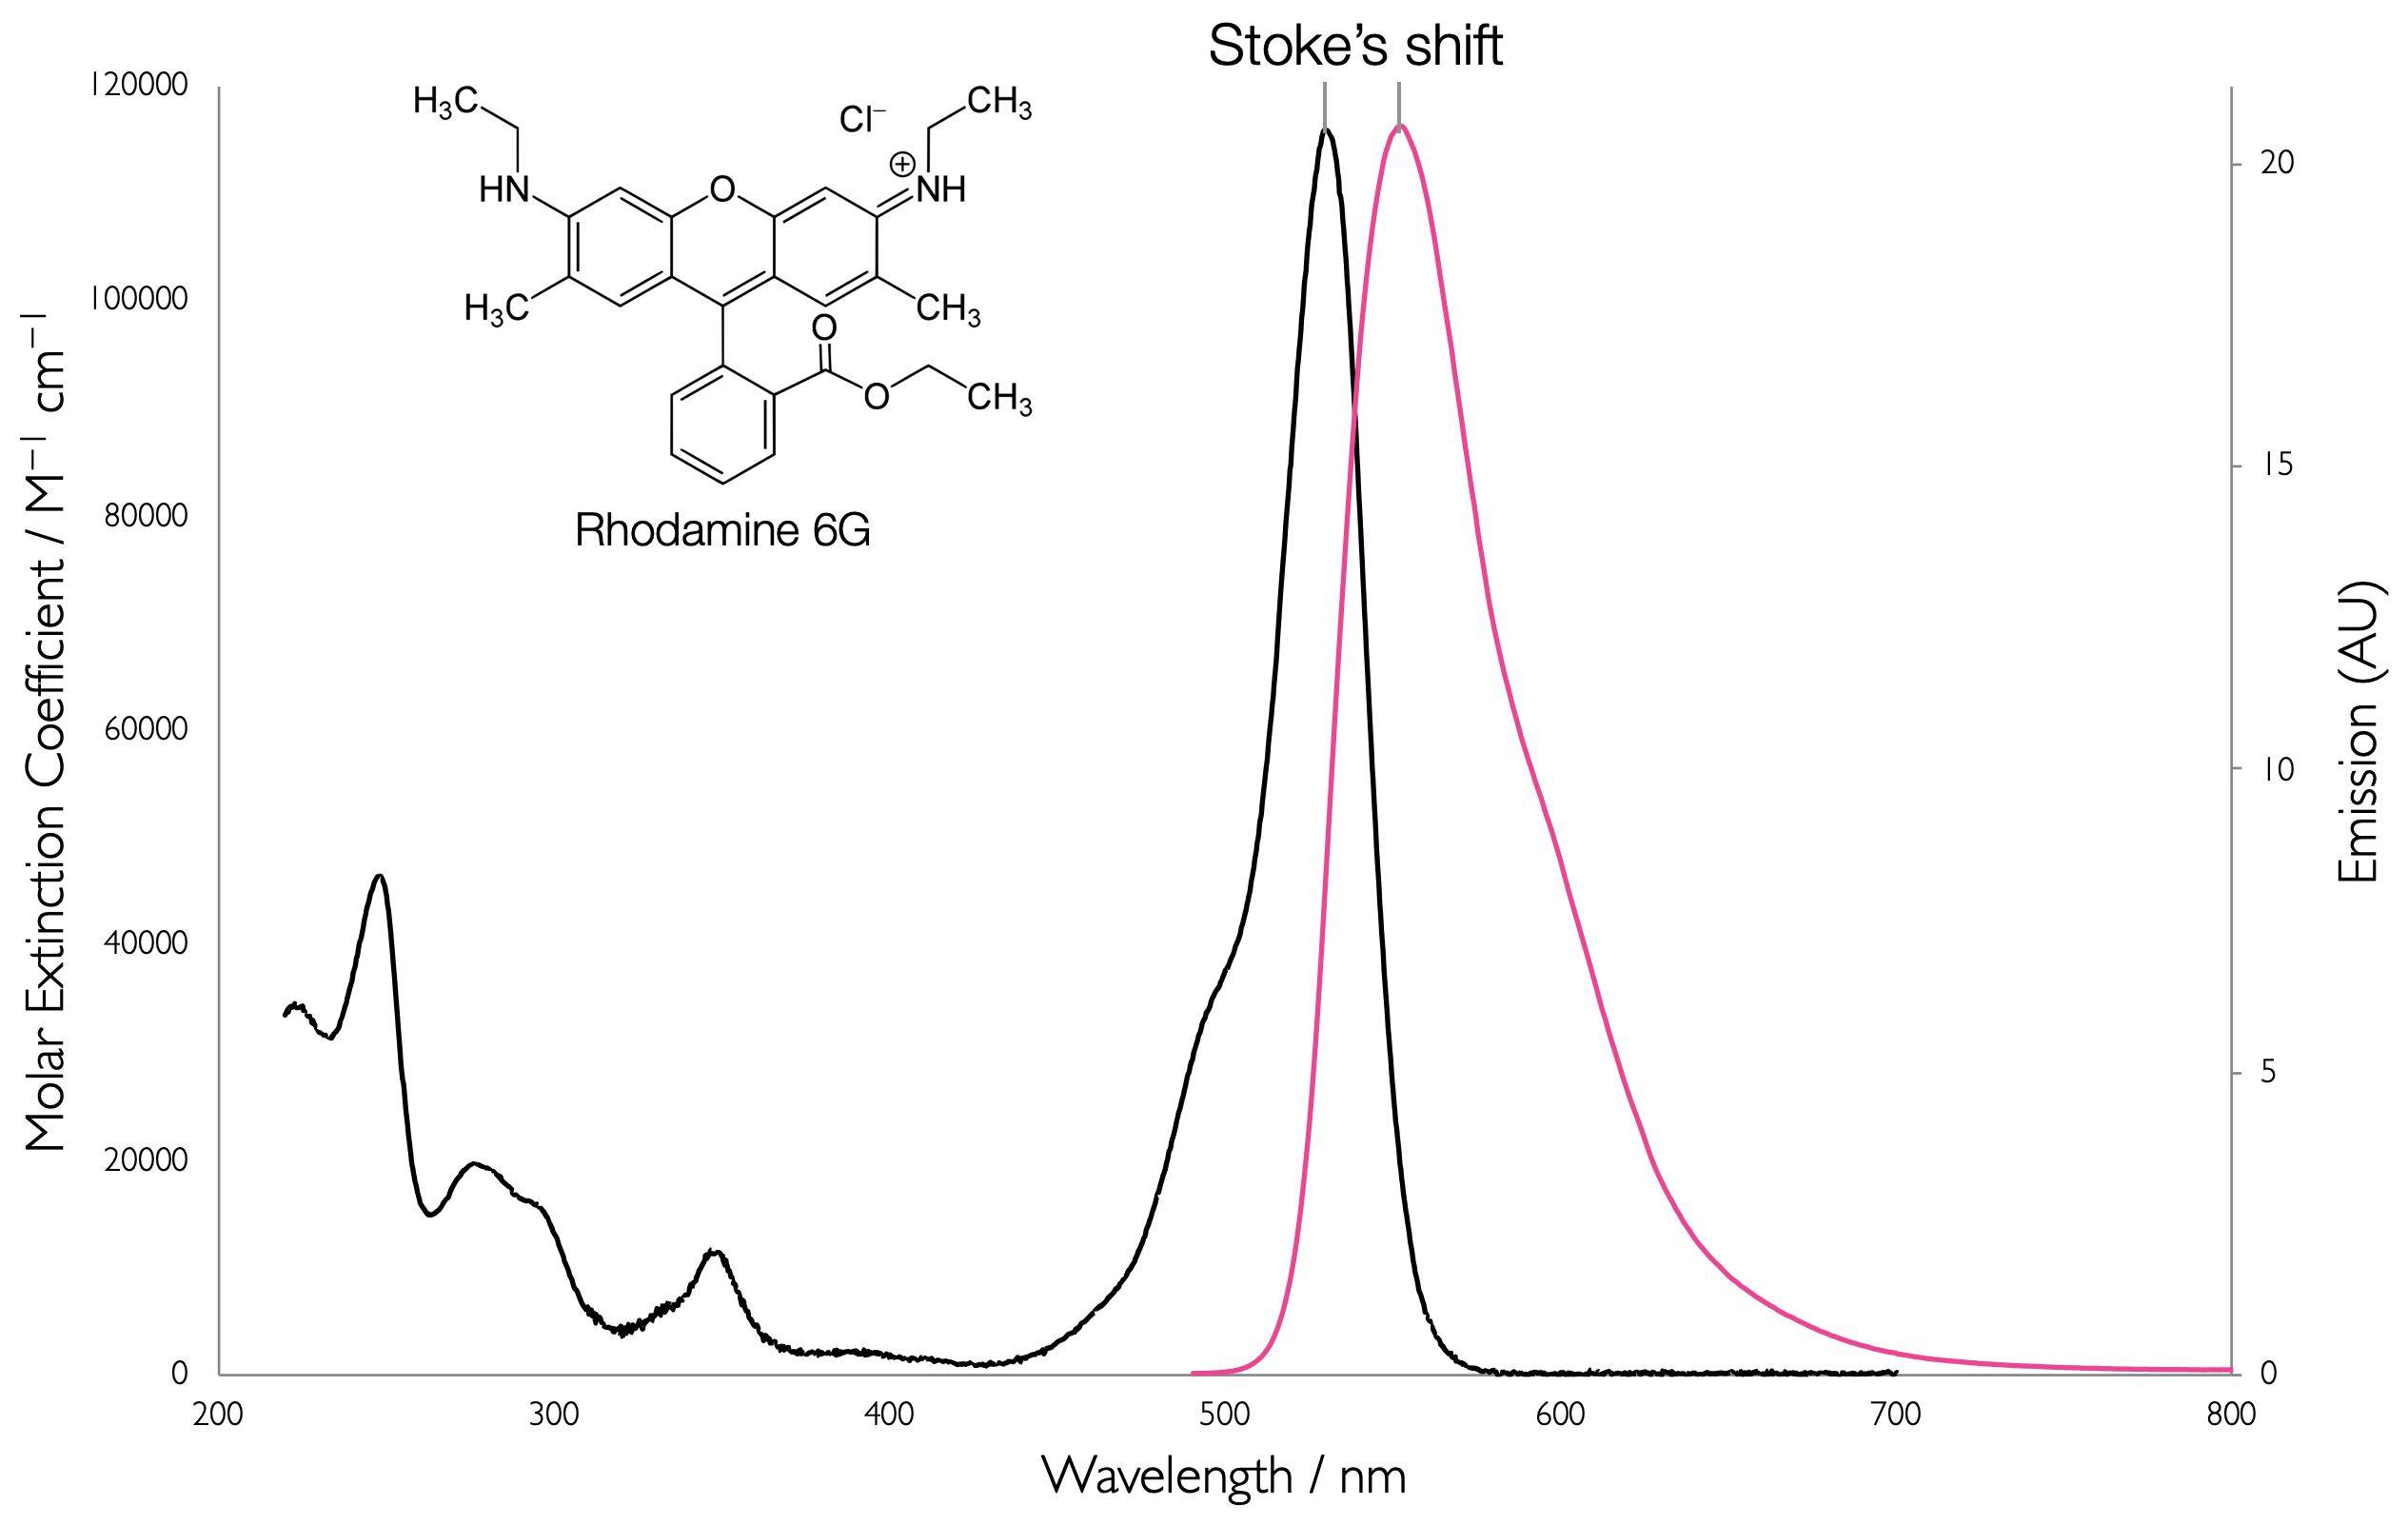
\includegraphics[width=0.7\linewidth]{images/stokesspectrum} 

}

\caption{The absorption and emission spectra of rhodamine 6G showing the Stokes shift of the two spectra.[Data from [OMLC](https://omlc.org/spectra/PhotochemCAD/html/083.html), accessed July 2020]}\label{fig:stokesspectrum}
\end{figure}

The axis title of 'reaction coordinate' is used ubiquitously, but is poorly understood. The simple idea that a bond becomes longer (as would be the case for a diatomic molecule) does not apply as we are considering the whole molecule.

The Stokes shift can be far more easily accounted for if we consider what is going on in the molecule. Initially the molecule exists in a state optimised for for that state, the shape and structure of the dye molecule and the arrangement of solvent around it are all minimised to give the lowest energy configuration. We shall consider the most simple case of the transitions between the ground vibrational states of the HOMO \& LUMO.

Absorption of a photon is a very fast process, in the order of femtoseconds, and is significantly faster than molecular vibrations or structural reorganisation. Consequently the molecule becomes excited into a state which has exactly the same structural configuration and salvation shell as the ground state, however this is now no longer the most optimal state, figure \ref{fig:stokesenergy}.

\begin{figure}

{\centering \includegraphics[width=0.8\linewidth]{images/stokesenergy} 

}

\caption{Sketch of the photophysical processes involved in the Stokes shift of emission. The ground state structure of the dye and solvent sphere (lower left) is maintained upon almost instantaneous absorption of a photon, however this then relaxes to an optimised configuration of dye and solvent for the excited state (top right), however this destabilises the ground state.}\label{fig:stokesenergy}
\end{figure}

Since the excited state is relatively stable (ns) when compared with the time taken for vibrations and molecular restructuring (ps) the excited state dye molecule and the solvent will reorganise to minimise the energy of the excited state, however in doing so this destabilises the ground state of the molecule. The actual process of emission is again very fast (ps) and so there is no opportunity for the structure of the chromophore or solvation sphere to reorganise. Upon deactivation this state, optimised for the excited state reorganises, lowering the energy of the ground state and destabilising the excited state.

As a consequence of this stabilising action of the ground and excited states the energy gap of absorption is larger than the energy gap of emission, or the emission of a photon is redshifted from the absorption. This explains the origin of Stokes shift, and explains the offset the Morse curves of the ground and excited states which have previously been used to explain the origin of the Stokes shift.

\hypertarget{sec:azuleneS2}{%
\section{\texorpdfstring{Emission from S\textsubscript{2}}{Emission from S2}}\label{sec:azuleneS2}}

Kasha's rule is almost always true, but there are known exceptions to this rule, one of these examples is azulene. Azulene has a broad absorption band between 500-600 nm, however emission from this molecule occurs at below 400 nm. If we look at figure \ref{fig:azulene} which shows the absorption and emission spectra of azulene it can be seen that the emission spectra is a mirror image of S\textsubscript{0}-S\textsubscript{2} (excitation into the second excited electronic state) absorption band, indicating the emission is also from the S\textsubscript{2} to S\textsubscript{0} states.

\begin{figure}

{\centering 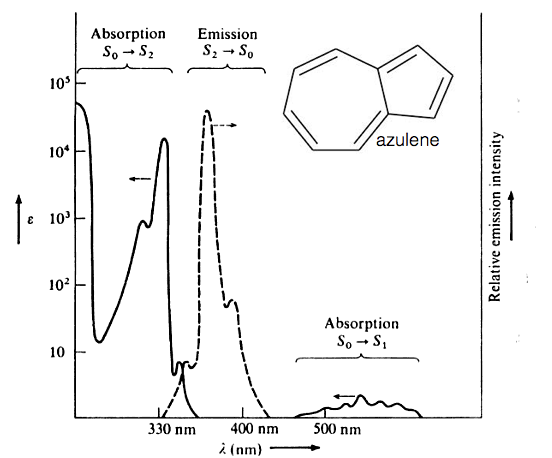
\includegraphics[width=0.6\linewidth]{images/azulene} 

}

\caption{The absorption (solid line) and emission (dashed line) spectrum of azulene in ethanol. Note the emission appears in the near UV part of the spectrum. }\label{fig:azulene}
\end{figure}

The molar extinction coefficient is also significantly higher for this S\textsubscript{0}-S\textsubscript{2} absorption indicating a much greater overlap integral of these two states.

What causes the unusual photophysical example? In short there is a very large energy gap between the S\textsubscript{2} and S\textsubscript{1} excited states this has the effect of greatly reducing the rate of internal conversion. There is a very weak emission from the S\textsubscript{1} to S\textsubscript{0}, in this case the energy gap is relatively small and there is an efficient deactivation of the excited state by internal conversion.

\hypertarget{sec:ratesphoto}{%
\section{Rates of Photophysical Processes \& Quantum Yield}\label{sec:ratesphoto}}

Fluorescence (and phosphorescence) are first order processes, just like radioactive decay. The probability of a molecule decaying from an excited state depends only the concentration of that excited state, \([A^\ast]\).

Rate of decay of \([A^\ast]\):

\begin{equation}
\frac{\textrm{d}[A^\ast]}{\textrm{d}t}=-k_f [A^\ast]
\label{eq:fluordecay}
\end{equation}

It is usual to refer to the `lifetime' of photophysical processes, and it is a term already used at the start of this chapter, the lifetime of a process, usually given the symbol τ, is the reciprocal of the rate constant for that process, so τ\textsubscript{f} = 1/k\textsubscript{f}. Often the natural lifetime of a dye is used, this assumes that there are no other deactivation pathways from the excited state and all of the energy is lost as fluorescence (or the fluorescence quantum yield is 1). The natural lifetime of fluorescence is given the symbol τ\textsubscript{f}\textsuperscript{0}, it is the maximum a lifetime can be and is solvent dependent.

If there is more than one possible deactivation pathway from the excited state is is often useful to be able to quantify these values. The quantum yield of a process describes the efficiency of each process, when a molecule absorbs a photon of light it generates an excited state; there are a number of different ways the molecule can decay from this excited state (see section \ref{sec:FluorPhos}, figure \ref{fig:Jablonski}). The quantum yield for each process is essentially the ratio of reactions proceeding down each pathway and the number of photons absorbed, quantum yield has no units.

\begin{equation}
\phi = \frac{\textrm{number of reactions proceeding down a given pathway}}{\textrm{number of photons absorbed}}
\label{eq:QYdef}
\end{equation}

\begin{longtable}[]{@{}llll@{}}
\caption{\label{tab:QYtab} The deactivation pathways of an excited state, with the associated rate constants and quantum yields.}\tabularnewline
\toprule
\begin{minipage}[b]{0.33\columnwidth}\raggedright
\strut
\end{minipage} & \begin{minipage}[b]{0.24\columnwidth}\raggedright
\strut
\end{minipage} & \begin{minipage}[b]{0.16\columnwidth}\raggedright
Rate of Process\strut
\end{minipage} & \begin{minipage}[b]{0.16\columnwidth}\raggedright
Quantum Yield\strut
\end{minipage}\tabularnewline
\midrule
\endfirsthead
\toprule
\begin{minipage}[b]{0.33\columnwidth}\raggedright
\strut
\end{minipage} & \begin{minipage}[b]{0.24\columnwidth}\raggedright
\strut
\end{minipage} & \begin{minipage}[b]{0.16\columnwidth}\raggedright
Rate of Process\strut
\end{minipage} & \begin{minipage}[b]{0.16\columnwidth}\raggedright
Quantum Yield\strut
\end{minipage}\tabularnewline
\midrule
\endhead
\begin{minipage}[t]{0.33\columnwidth}\raggedright
Absorption\strut
\end{minipage} & \begin{minipage}[t]{0.24\columnwidth}\raggedright
\(S_0 + h \nu \longrightarrow S_1\)\strut
\end{minipage} & \begin{minipage}[t]{0.16\columnwidth}\raggedright
\(I\)\strut
\end{minipage} & \begin{minipage}[t]{0.16\columnwidth}\raggedright
\strut
\end{minipage}\tabularnewline
\begin{minipage}[t]{0.33\columnwidth}\raggedright
Fluorescence\strut
\end{minipage} & \begin{minipage}[t]{0.24\columnwidth}\raggedright
\(S_1 \longrightarrow S_0 + h \nu'\)\strut
\end{minipage} & \begin{minipage}[t]{0.16\columnwidth}\raggedright
\(k_f[S_1]\)\strut
\end{minipage} & \begin{minipage}[t]{0.16\columnwidth}\raggedright
\(\phi _f\)\strut
\end{minipage}\tabularnewline
\begin{minipage}[t]{0.33\columnwidth}\raggedright
Internal conversion\strut
\end{minipage} & \begin{minipage}[t]{0.24\columnwidth}\raggedright
\(S_1 \longrightarrow S_0 + \textrm{heat}\)\strut
\end{minipage} & \begin{minipage}[t]{0.16\columnwidth}\raggedright
\(k_{ic}[S_1]\)\strut
\end{minipage} & \begin{minipage}[t]{0.16\columnwidth}\raggedright
\(\phi _{ic}\)\strut
\end{minipage}\tabularnewline
\begin{minipage}[t]{0.33\columnwidth}\raggedright
Intersystem crossing \emph{singlet to triplet}\strut
\end{minipage} & \begin{minipage}[t]{0.24\columnwidth}\raggedright
\(S_1 \longrightarrow T_1 + \textrm{heat}\)\strut
\end{minipage} & \begin{minipage}[t]{0.16\columnwidth}\raggedright
\(k_{ST}[S_1]\)\strut
\end{minipage} & \begin{minipage}[t]{0.16\columnwidth}\raggedright
\(\phi _{ST}\)\strut
\end{minipage}\tabularnewline
\begin{minipage}[t]{0.33\columnwidth}\raggedright
Phosphorescence\strut
\end{minipage} & \begin{minipage}[t]{0.24\columnwidth}\raggedright
\(T_1 \longrightarrow S_0 + h \nu''\)\strut
\end{minipage} & \begin{minipage}[t]{0.16\columnwidth}\raggedright
\(k_p[T_1]\)\strut
\end{minipage} & \begin{minipage}[t]{0.16\columnwidth}\raggedright
\(\phi _p\)\strut
\end{minipage}\tabularnewline
\begin{minipage}[t]{0.33\columnwidth}\raggedright
Intersystem crossing \emph{internal conversion triplet to singlet}\strut
\end{minipage} & \begin{minipage}[t]{0.24\columnwidth}\raggedright
\(T_1 \longrightarrow S_0 + \textrm{heat}\)\strut
\end{minipage} & \begin{minipage}[t]{0.16\columnwidth}\raggedright
\(k_{TS}[T_1]\)\strut
\end{minipage} & \begin{minipage}[t]{0.16\columnwidth}\raggedright
\(\phi _{TS}\)\strut
\end{minipage}\tabularnewline
\bottomrule
\end{longtable}

According to the Stark-Einstein law the total quantum yield of all processes is unity (one), however if secondary reactions occur (such as radical propagation) it may be more than 1. The quantum yield and rate of a process are intrinsically linked. It should be implicit that the faster the rate of a process (the bigger the rate constant) the bigger the quantum yield of that process; in fact the quantum yield of a process, such as fluorescence, is the rate of fluorescence divided by the sum of the rates of all of the deactivation processes (equation \eqref{eq:QYfluor}).

\begin{equation}
\phi_f = \frac{k_f^0}{k_f^0+k_{ic}+ k_{ST}+k_{\textrm{other}}}
\label{eq:QYfluor}
\end{equation}

(Examples of expressions for other processes may be found in Section \ref{sec:SSQemissionans} equations \eqref{eq:QYIC}, \eqref{eq:QYST} \& \eqref{eq:QYTS}.)

When there are more processes occurring then the singlet lifetime (sometimes called the fluorescence lifetime) will be smaller than the natural fluorescence lifetime, because now the denominator term is bigger (equation \eqref{eq:lifetimefluor}).

\begin{equation}
\tau_S = \frac{1}{k_f^0+k_{ic}+ k_{ST}+k_{\textrm{other}}}
\label{eq:lifetimefluor}
\end{equation}

If we assume that there is no quenching of the system (this is discussed later) and no chemistry the only decay pathways from the excited state are emission (fluorescence), internal conversion and intersystem crossing to the triplet state, and so consequently only these terms would appear in the equation for the quantum yield. Processes that occur from the triplet state are independent, and therefore none of these terms occur in quantum yield or lifetime equations from the singlet, fluorescent state.

For processes that occur from the triplet state, then obviously, the quantum yield will depend upon the total number of triplet states produced, which is given by the quantum yield of intersystem crossing. So the quantum yield of phosphorescence is given by:

\begin{equation}
\phi_p = \frac{k_p^0}{k_p^0+k_{TS}+k_{\textrm{other}}}
\label{eq:QYphos}
\end{equation}

Quantum yields of photophysical processes can be difficult to measure, in part because it is difficult to easily quantify the number of photons going into a sample, and because emission occurs at all angles from the sample. A technique called `actinometry' is usually used where the emission from an unknown sample is compared with that of a well characterised sample.

A good actinometer should have a good overlap in both the absorption and emission spectra, a high molar absorption coefficient, it should be photochemically stable and have a high emission quantum yield, a selection of well characterised actinometers are included in figure \ref{tab:actinometer}. Measurements on the absorption at the excitation wavelength, and the full emission spectra are required for both the unknown and the actinometer, as well as details on the reactive index of the solvents used. For best results a monochromatic light source should be used (a laser) and the same excitation wavelength must be used for both samples; the absorbance of the solutions should also be low (\textless0.1).

Usually emission spectra are measured as intensity against wavelength, but when `integrating' the emission of the unknown and actinometer it is important that they are integrated over a linear space (energy or frequency) which can make calculations more difficult (but perfectly doable in something like Excel). Equation \eqref{eq:actinometry} shows the relationship between the fluorescence quantum yield of an unknown, Φ, with that of a reference actinometer, Φ\textsubscript{R}. A is the absorbance at the excitation wavelength, and n the refractive index of the solvent. Here, because all terms appear as ratios there is no need to worry about units with anything.

\begin{equation}
\phi=\phi_R \frac{\int{I}\textrm{d}\bar \nu}{\int{I_R}\textrm{d}\bar \nu}\frac{A_R}{A}\frac{n^2}{n^2_R}
\label{eq:actinometry}
\end{equation}

The integrated emission intensity, \(\int{I}\textrm{d}\bar \nu\), of the unknown and reference is here shown as being integrated over wavenumber, but so long as it is integrated over linear space\footnote{The term linear space implies the steps are the same size, energy is the more fundamental unit, since wavelength is a reciprical function of energy wavelength space is non linear.} it does not matter if frequency or energy is used instead as any units from the terms cancel.

\begin{longtable}[]{@{}lllll@{}}
\caption{\label{tab:actinometer} The photophysical details of well characterised actinometers.}\tabularnewline
\toprule
Reference & Solvent & λ\textsubscript{ex}/nm & Φ\textsubscript{em} & λ\textsubscript{em,max} / nm\tabularnewline
\midrule
\endfirsthead
\toprule
Reference & Solvent & λ\textsubscript{ex}/nm & Φ\textsubscript{em} & λ\textsubscript{em,max} / nm\tabularnewline
\midrule
\endhead
quinine sulfate & 0.1 M H\textsubscript{2}SO\textsubscript{4} & 350 & 0.577 & 444\tabularnewline
fluorescein & 0.1 M H\textsubscript{2}SO\textsubscript{4} & 496 & 0.95 & 521\tabularnewline
rhodamine 6G & ethanol & 488 & 0.94 & 530\tabularnewline
cresyl violet & methanol & 540 & 0.54 & 622\tabularnewline
\bottomrule
\end{longtable}

\hypertarget{fluorescence-lifetime}{%
\section{Fluorescence lifetime}\label{fluorescence-lifetime}}

Spontaneous emission (either fluorescence or phosphorescence) from an excited state is a first order process, and so shows similar kinetics to that which you have already studied, figure \ref{fig:fluorlifetime} \& equation \eqref{eq:fluorlifetime}.

\begin{figure}

{\centering 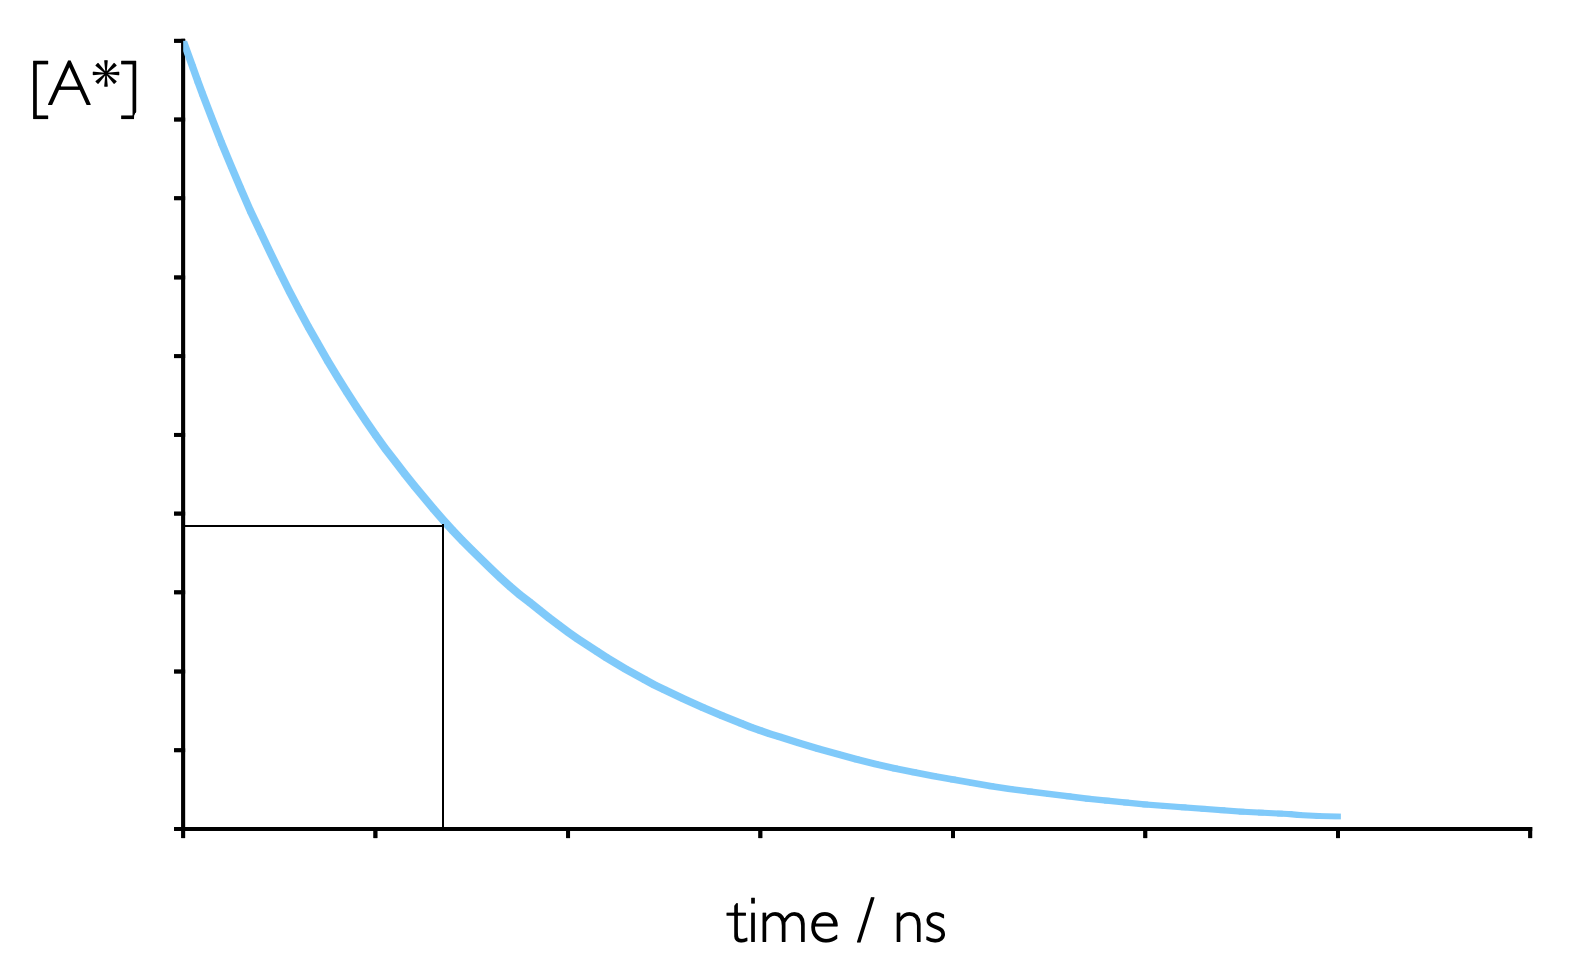
\includegraphics[width=0.5\linewidth]{images/fluorlifetime} 

}

\caption{Emission from an excited state is a first order process, whereby an excited state decays spontaneously. The emission lifetime is the time required for the concentratio of an excited state to fall to 1/e of its initial value.}\label{fig:fluorlifetime}
\end{figure}

However, instead of using rate constants when talking about this decay (as seen in Section \ref{sec:ratesphoto} photochemists tend to talk about emission lifetimes, \(\tau\).

The fluorescence lifetime is defined as the time required for the concentration of excited state to fall to 1/e (\textasciitilde0.3679) of the initial concentration.

So for an excited singlet state the fluorescence lifetime is related to the concentrations as follows:

\begin{equation}
[S_1]_t=[S_1]_0e^-{\frac{t}{\tau}}
\label{eq:fluorlifetime}
\end{equation}

where \(\tau\) is the value given in equation \eqref{eq:lifetimefluor}.

\hypertarget{before-completing-this-section}{%
\section{Before Completing this Section}\label{before-completing-this-section}}

To support the material in this section it is suggested you read chapters 3 \& 4 of Wardle `Principles and Application of Photochemistry'.

\hypertarget{ch:Workshop2}{%
\chapter{Workshop Questions for Week 3}\label{ch:Workshop2}}

\hypertarget{sec:YieldLifetime}{%
\section{Short mathematical question - Quantum Yield and lifetime}\label{sec:YieldLifetime}}

The quantum yield and lifetime of a dye were measured to be 0.43 \& 2.6 ns respectively. What is the natural lifetime?

\emph{(I will use MCQs and UniDoodle to ask this in class)}

\hypertarget{sec:otherprocesses}{%
\section{Short conceptual question - Effect of other processes}\label{sec:otherprocesses}}

For a given value of τ\textsubscript{0} what happens to the lifetime and quantum yield as k\textsubscript{IC} and k\textsubscript{ISC} increases?

\emph{(This will be a discussion question)}

\hypertarget{sec:structure}{%
\section{Conceptual question - Effect of structure}\label{sec:structure}}

Fluorescein (figure \ref{fig:fluorescein}) in basic aqueous solution has a quantum yield of fluorescence, Φ\textsubscript{f}, of 0.95, and fluorescence lifetime, τ\textsubscript{f}, of 4.1 ns.

\begin{figure}

{\centering 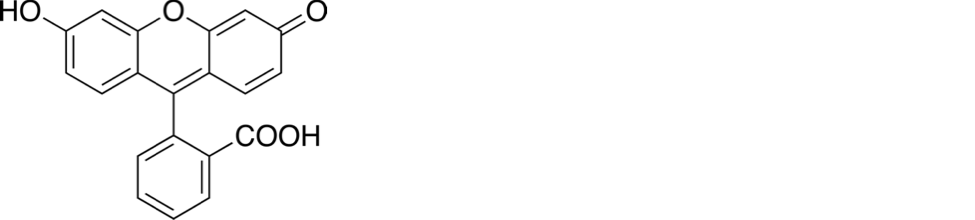
\includegraphics[width=0.7\linewidth]{images/fluorescein} 

}

\caption{The structure of the fluorescent molecule fluorescein}\label{fig:fluorescein}
\end{figure}

\emph{(This will be a discussion question)}

\hypertarget{conceptual-question---lack-of-symmetry-in-spectra.}{%
\section{Conceptual question - lack of symmetry in spectra.}\label{conceptual-question---lack-of-symmetry-in-spectra.}}

The absorption and emission spectrum of fluorescein is shown in figure (\ref{fig:fluoresceinspec})

\begin{figure}

{\centering 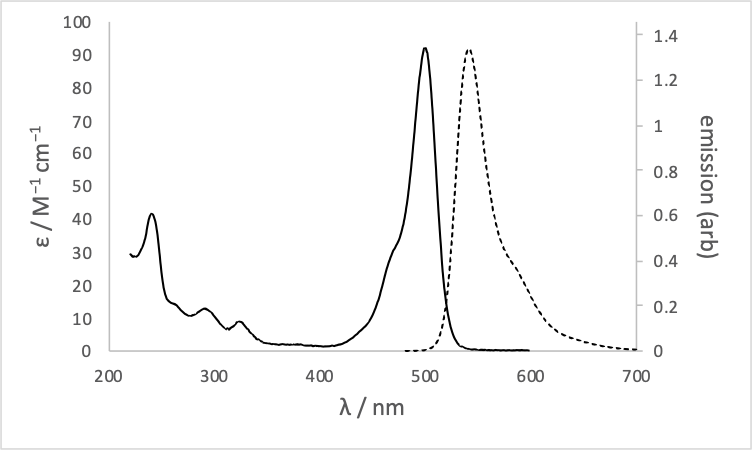
\includegraphics[width=0.7\linewidth]{images/fluoresceinspec} 

}

\caption{The absorption (solid) and emission (dashed) spectrum of fluorescein in basic ethanol.}\label{fig:fluoresceinspec}
\end{figure}

Why are the absorption bands between 200 -- 350 nm not reflected in the emission spectrum?

\hypertarget{sec:stokes}{%
\section{Conceptual question - Stokes' shift}\label{sec:stokes}}

The inorganic dye {[}Ru(bpy)\textsubscript{3}{]}\textsuperscript{2+} has a measured lifetime in water of 580 ns and a natural lifetime of 13.8 µs. The spectrum is shown in figure \ref{fig:Rubpyspec}. What is the origin of the large Stokes' shift in this system?

\begin{figure}

{\centering 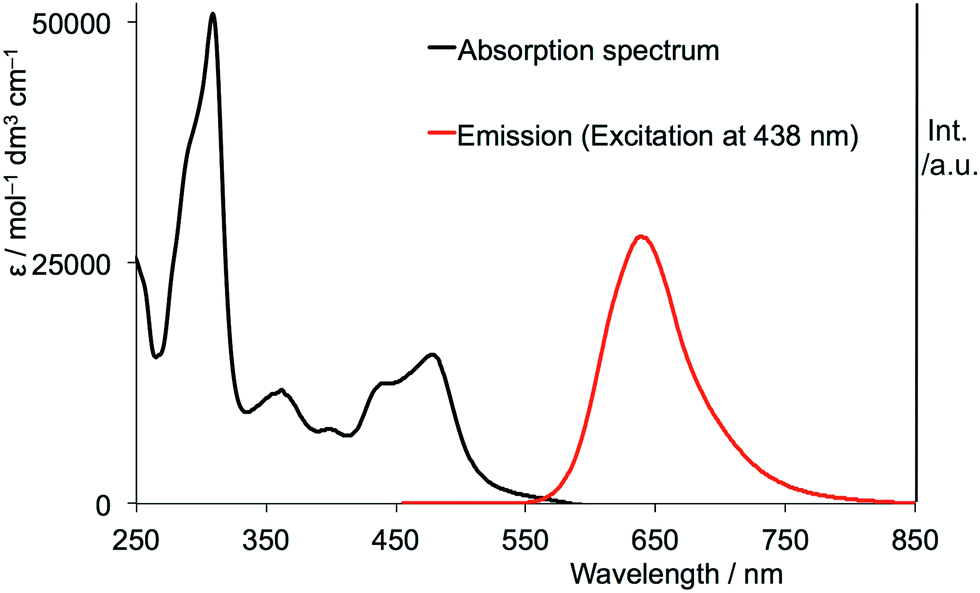
\includegraphics[width=0.7\linewidth]{images/Rubpy3spectra} 

}

\caption{The absorption (black) and emission (red) spectrum of ruthenium tris bypyridine in water.}\label{fig:Rubpyspec}
\end{figure}

Data from Shi \emph{et al.}, Synthesis and characterization of phosphorescent two coordinate copper(I) complexes bearing diamidocarbene ligands. \href{https://doi.org/10.1039/C6DT04016K}{Dalton Trans., 2017,46, 745-752.}

\hypertarget{sec:binding}{%
\section{Conceptual question - the effect of binding on emission}\label{sec:binding}}

The asymmetric cyanine dye YO-Pro-1 is a DNA stain because it has a large increase on fluorescence emission when binding to DNA. The lifetime in free solution is around 2 ps and when bound to DNA is 2.4 ns. What is the structural origin of the large increase of emission upon binding?

\begin{figure}

{\centering 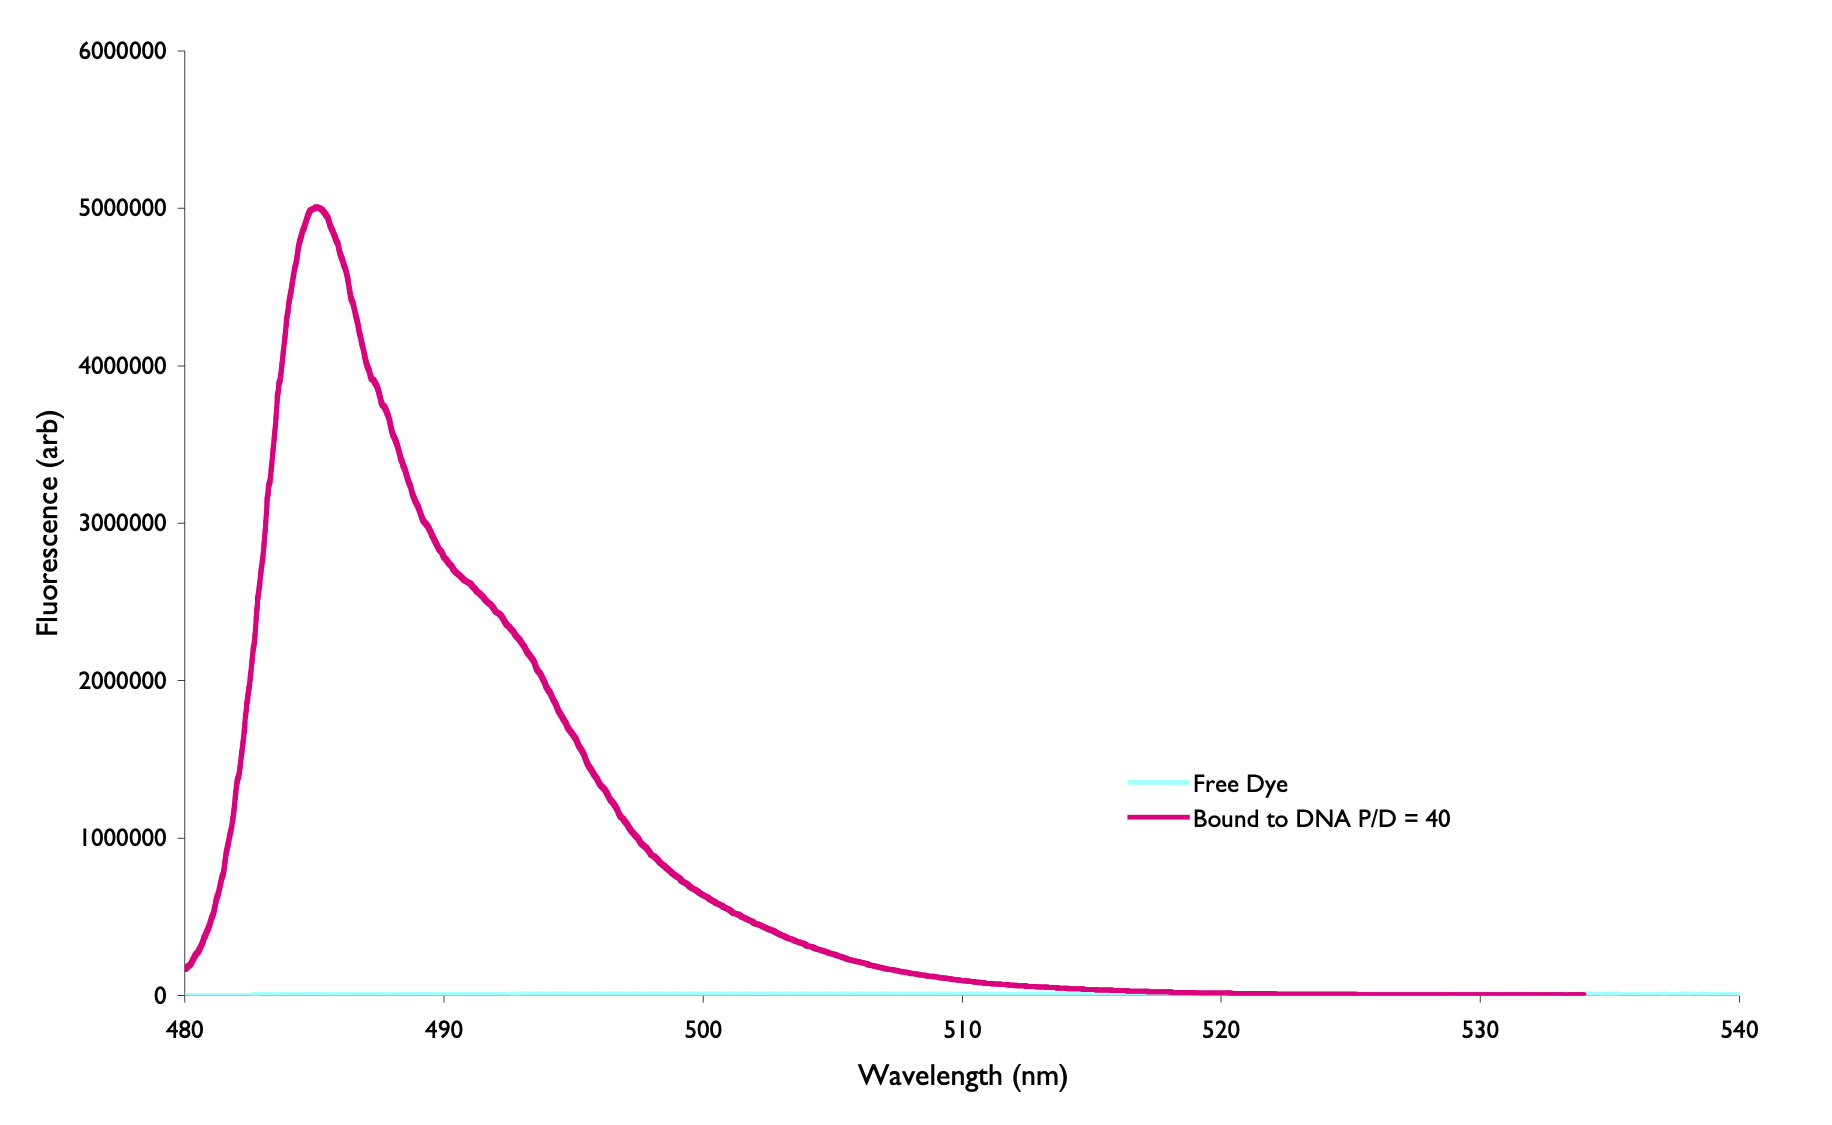
\includegraphics[width=0.7\linewidth]{images/YODNA} 

}

\caption{The emission spectrum of the choromophore YO-Pro-1 when free in aqueous solution (blue) and when bound to DNA (pink)}\label{fig:YODNA}
\end{figure}

\emph{(This will be a discussion question)}

\hypertarget{extended-question---properties-of-ethidium-bromide-example-exam-question}{%
\section{Extended question - Properties of Ethidium Bromide (Example Exam Question)}\label{extended-question---properties-of-ethidium-bromide-example-exam-question}}

Ethidium bromide (EB, figure \ref{fig:ethidiumstructure} is used as a DNA stain, which is essentially non-fluorescent in aqueous solution, but shows a strong enhancement of emission upon binding to double stranded DNA (which has a negatively charged backbone).

Emission is almost exclusively from the singlet excited state, but a triplet state has been shown to exist, which emits with a low quantum yield (Φ\textsubscript{P} = 0.00006).

\begin{figure}

{\centering 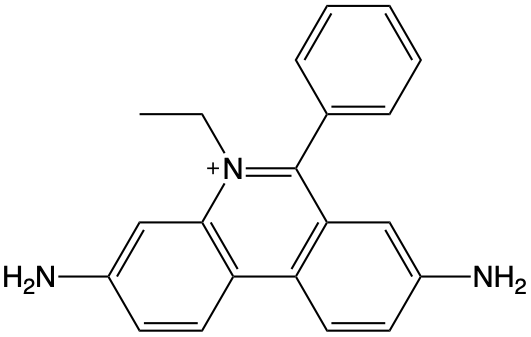
\includegraphics[width=0.3\linewidth]{images/ethidiumstructure} 

}

\caption{The structure of the cationic ethidium bromide chromophore.}\label{fig:ethidiumstructure}
\end{figure}

\begin{itemize}
\item
  Sketch a Jablonski diagram for the processes you know to occur.
\item
  The molar extinction coefficient, ε, of EB has be measured to be 78500 M\textsuperscript{−1} cm\textsuperscript{−1}. What factors contribute to EB having such a high extinction coefficient?
\end{itemize}

The following spectra, lifetimes and quantum yield have been measured for EB in different free solution and DNA systems:

\begin{longtable}[]{@{}lll@{}}
\caption{\label{tab:ethidiumlifetime} The lifetimes and quantum yields of ethidium bromide in aquous solution and when bound to DNA in protiated and deuterated systems.}\tabularnewline
\toprule
& τ / ns & Φ\textsubscript{f}\tabularnewline
\midrule
\endfirsthead
\toprule
& τ / ns & Φ\textsubscript{f}\tabularnewline
\midrule
\endhead
H\textsubscript{2}O (no DNA) & 1.6 & 0.012\tabularnewline
D\textsubscript{2}O (no DNA) & 6.3 &\tabularnewline
DNA & 28.3 & 0.220\tabularnewline
DNA (deuterated) & 38.4 &\tabularnewline
\bottomrule
\end{longtable}

\begin{figure}

{\centering 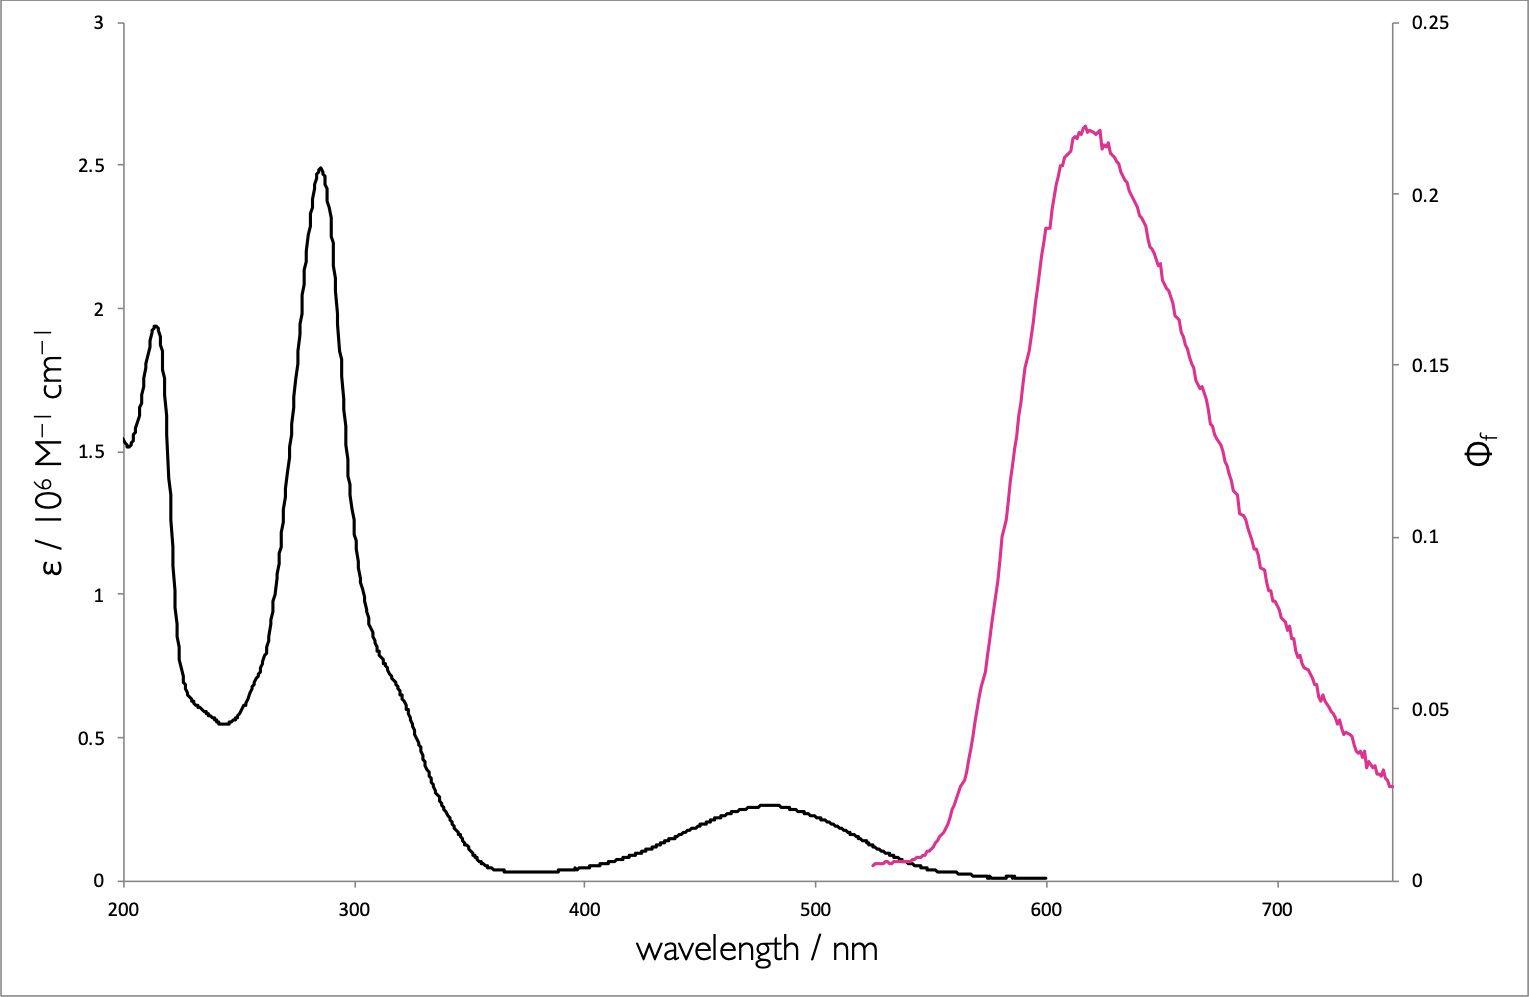
\includegraphics[width=0.3\linewidth]{images/ethidiumspectra} 

}

\caption{The absorption (black) and emission (pink) spectrum of ethidium bromide when bound to DNA.}\label{fig:ethidiumspectra}
\end{figure}

\begin{itemize}
\item
  What factors likely lead to an enhancement of fluorescence quantum yield upon binding to DNA?
\item
  Show that the natural lifetime of EB is 129 ns.
\item
  What is the origin of the large Stoke's shift (λ\textasciitilde max ex\textasciitilde{} = 520 nm, λ\textasciitilde max em\textasciitilde{} = 608 nm)
\item
  What transitions are responsible for the absorption features in the:
  * 400-600 nm range
  * 200-350 nm range
\item
  Why are the features in the 200-350 nm range not replicated in the emission spectrum?
\item
  Why does deuterating the solvent (or DNA) effect the lifetime of the excited state?
\item
  What effect would freezing the samples have on the lifetime, fluorescence quantum yield \& phosphorescence quantum yield.
\end{itemize}

A study of the thermodynamics of the dye DNA system measured the binding constant of EB with DNA to be 1.05 × 10\textsuperscript{6}.

\begin{itemize}
\item
  Why is the measured quantum yield for a system containing 2 µM EB and 20 mM DNA only 0.18?
\item
  Why would increasing the ionic strength of the solution, increase the fluorescence intensity of EB in solution with DNA?
\end{itemize}

\hypertarget{short-conceptual-question---effect-of-polar-solvents-on-emission}{%
\section{Short conceptual question - effect of polar solvents on emission}\label{short-conceptual-question---effect-of-polar-solvents-on-emission}}

Solutions containing anthracence and diethylaniline are shown to have broad emission at around 450 nm in toluene, but in dichloromethane no emission is observed.

The emission from athracene has λ\textsubscript{max} of 375 nm.

Suggest the processes going on which account for these observations.

\hypertarget{ch:Quench}{%
\chapter{Non-emmisive Deactivation of the Excited State}\label{ch:Quench}}

\hypertarget{sec:QuenchLOs}{%
\subsection{Learning Objectives}\label{sec:QuenchLOs}}

At the end of this section you should be able to:

\begin{itemize}
\tightlist
\item
  Discuss the heavy atom effect.
\item
  Understand the difference between static and dynamic quenching.
\item
  Graphically determine quenching constants for static, dynamic and mixed method quenching.
\item
  Describe mathematically the effect of quenching on emission quantum yields and lifetime.
\item
  Describe the mechanisms of non-collisional energy transfer.
\item
  Demonstrate understanding of the factors which affect the rates of non-collisional energy transfer.
\end{itemize}

\hypertarget{sec:energygap}{%
\section{The Energy Gap Law}\label{sec:energygap}}

The natural lifetime of fluorescence assumes that there is no other available pathway for deactivation of the excited state. However, the effects of internal conversion and intersystem crossing have already been seen by the presence of rate constants for internal conversion (IC) and intersystem crossing (ST) in the equations for quantum yield of fluorescence. The rate of non-radiative decay is given by the energy gap law (a formalised equation is not given here) which depends upon a number of factors but principally the energy gaps (ΔE) between electronic levels.

Non radiative decay become increasingly unfavourable as the energy gaps become bigger, and the rate of non-radiative decay decreases exponentially with increasing energy gaps. The energy gaps between higher electronic states (S\textsubscript{2}, S\textsubscript{3}, S\textsubscript{4} \emph{etc.}) are usually significantly smaller than the S\textsubscript{1} - S\textsubscript{0} energy gap leading to rapid internal conversion down to the lowest (singlet) excited state, which is the origin of Kasha's rule.

\begin{longtable}[]{@{}llllll@{}}
\caption{\label{tab:actinometer} The lifetime of the excited state increases dramatically as the energy gap between the ground and excited state increases due to a decrease in internal conversion. The quantum yield of emission increases as the rate constant for internal conversion decreases..}\tabularnewline
\toprule
& λ\textsubscript{abs} / nm & λ\textsubscript{em} / nm & ΔE / eV & τ/ nw & Φ\textsubscript{em}\tabularnewline
\midrule
\endfirsthead
\toprule
& λ\textsubscript{abs} / nm & λ\textsubscript{em} / nm & ΔE / eV & τ/ nw & Φ\textsubscript{em}\tabularnewline
\midrule
\endhead
{[}Os(phen)\textsubscript{3}{]}\textsuperscript{2+} & 650 & 720 & 0.186 & 260 & 0.016\tabularnewline
{[}Os(phen)\textsubscript{2}(dppene){]}\textsuperscript{2+} & 455 & 609 & 0.69 & 1830 & 0.138\tabularnewline
{[}Os(phen)(dppene)\textsubscript{2}{]}\textsuperscript{2+} & 400 & 530 & 0.761 & 3600 & 0.518\tabularnewline
\bottomrule
\end{longtable}

The rate of non-radiative decay also depends upon the vibrations within a molecule (this should be logical since the energy is lost as heat), as well as the size of any structural changes required upon deactivation of the excited state. Since the frequency of vibrations is a factor in the rate of non-radiative decay there are clear isotope effects; particularly when hydrogens are replaced with deuteriums. C-H stretches occur with a frequency around 3000 cm\textsuperscript{−1}, whereas this is much lower at around 2200 cm\textsuperscript{−1} for C-D stretches; because of this the efficiency of vibrational relaxation in the hydrogen sample is considerably greater and the lifetime of the excited state is consequently longer in the deuterated sample.

Now a quantitive value may be determined for the rate of internal conversion it is easy to quantify the rate of intersystem crossing.

For intersystem crossing the efficiency is again determined by the size of the energy gap between the singlet and triplet states.

El Sayed's rule states:

\begin{quote}
the rate of intersystem crossing is relatively large if the radiationless transition involves a change in the orbital type.*
\end{quote}

Consequently intersystem crossing is considerably more efficient in molecules where there are hetero atoms as can be seen when comparing the rates of singlet triplet intersystem crossing between anthracene and 9-acetoanthracene, figure \ref{tab:rateST}. However, the presence of a hetero atom does not guarantee a high rate of intersystem crossing, for systems where there is no change in orbital type there rate constants are in the order of 100 to 1000 times more slow than those with a change in orbital type.

\begin{longtable}[]{@{}llll@{}}
\caption{\label{tab:rateST} The rates of intersystem crossing for a range of organic chromophores illustrating El Sayed's rule. When orbitals are listed as (for example) π,π* then it is looking at the pair of electrons in the highest orbitals (the valence HOMO electrons in the ground state), upon excitation an electron is excited from the π to the π* orbital.}\tabularnewline
\toprule
& transition & transition type & k\textsubscript{ST} / s\textsuperscript{−1}\tabularnewline
\midrule
\endfirsthead
\toprule
& transition & transition type & k\textsubscript{ST} / s\textsuperscript{−1}\tabularnewline
\midrule
\endhead
anthracene & S\textsubscript{1} (π,π*) ⟶ T\textsubscript{1} (π,π*) & forbidden & 1.4 × 10\textsuperscript{8}\tabularnewline
acetone & S\textsubscript{1} (n,π*) ⟶ T\textsubscript{1} (n,π*) & forbidden & 5 × 10\textsuperscript{8}\tabularnewline
benzil & S\textsubscript{1} (n,π*) ⟶ T\textsubscript{1} (n,π*) & forbidden & 5 × 10\textsuperscript{8}\tabularnewline
biacetyl & S\textsubscript{1} (n,π*) ⟶ T\textsubscript{1} (n,π*) & forbidden & 7 × 10\textsuperscript{7}\tabularnewline
9-acetoanthracence & S\textsubscript{1} (π,π*) ⟶ T\textsubscript{1} (n,π*) & allowed & \textasciitilde10\textsuperscript{10}\tabularnewline
benzophenone & S\textsubscript{1} (π,π*) ⟶ T\textsubscript{1} (n,π*) & allowed & \textasciitilde10\textsuperscript{11}\tabularnewline
\bottomrule
\end{longtable}

\hypertarget{sec:Collisional}{%
\section{Collisional Deactivation of the Excited State}\label{sec:Collisional}}

The photophysical deactivation pathways described above (emission, internal conversion and intersystem crossing) are not the only ways to deactivate an excited state of a molecule, and you perhaps have already noted the use of kother in equations \eqref{eq:QYfluor} - \eqref{eq:QYphos}. Another common pathway of deactivation, particularly in the solution phase, is collisional deactivation commonly known as quenching.

Table \ref{tab:phototrans}, part of which is repeated below, details all of the possible decay pathways from an excited state. Quenching competes with other processes, and consequently reduces the lifetime and yield of emission processes.

\begin{longtable}[]{@{}ll@{}}
\toprule
\endhead
\begin{minipage}[t]{0.56\columnwidth}\raggedright
\emph{Other pathways}\strut
\end{minipage} & \begin{minipage}[t]{0.38\columnwidth}\raggedright
\strut
\end{minipage}\tabularnewline
\begin{minipage}[t]{0.56\columnwidth}\raggedright
Quenching of excited state\strut
\end{minipage} & \begin{minipage}[t]{0.38\columnwidth}\raggedright
\(S_1 + Q \longrightarrow S_0 + Q +heat\) \(S_1 + Q \longrightarrow S_0 + Q^\ast +heat\) \(T_1 + Q \longrightarrow S_0 + Q +heat\) \(T_1 + Q \longrightarrow S_0 + Q^\ast +heat\)\strut
\end{minipage}\tabularnewline
\bottomrule
\end{longtable}

Quenching of the excited state competes with emission from the excited state, consequently reducing the quantum yield of fluorescence (or phosphorescence).

This bi-molecular, second order quenching process follows Stern-Volmer kinetics, equation \eqref{eq:SternVolmer}, a derivation of which can be found in Wardle, p 88-90).

\begin{equation}
\frac{I_0}{I}=1 + k_q \tau _0 [Q]
\label{eq:SternVolmer}
\end{equation}

Where \(I_0 / I\) is the ratio of the unquenched and quenched steady state intensity of the emission. For dynamic quenching this value will also be the same as \(\phi _0 / \phi\) and \(\tau _0 / \tau\), the ratios of the quantum yield and lifetime respectively, equation \eqref{eq:SternVolmerdynamic}.

\begin{equation}
\frac{I_0}{I}=\frac{\phi_0}{\phi}=\frac{\tau_0}{\tau}=1 + k_q \tau _0 [Q]
\label{eq:SternVolmerdynamic}
\end{equation}

Since this is a second order term when it appears in the equations \eqref{eq:QYfluor} - \eqref{eq:QYphos}, it appears as \(k_q[Q]\), such as indicated in equation \eqref{eq:QYfluorquench}.

\begin{equation}
\phi_f = \frac{k_f^0}{k_f^0+k_{ic}+ k_{ST}+k_q[Q]}
\label{eq:QYfluorquench}
\end{equation}

It is often useful to know if the quenching is diffusion or activation controlled, reactions in the solution phase cannot occur faster than the diffusion controlled rate, with second order rate constant \(k_d\), as described in equation 19.

\begin{equation}
k_d = \frac{8RT}{3 \eta}
\label{eq:diffcontrol}
\end{equation}

where T is the absolute temperature, and η the viscosity of the solvent. (It should be noted that there is an issue with units here where a conversion from m\textsuperscript{3} to dm\textsuperscript{3} is required). Diffusion controlled rates in aqueous, methanol and ethanol solutions are normally in the order of 10\textsuperscript{10} mol\textsuperscript{−1} dm\textsuperscript{3}. Values of rate constant lower than this are termed as activation controlled as only a fraction of the collisions result in a quenching of the excited state of the molecule.

\hypertarget{sec:static}{%
\section{Static Quenching}\label{sec:static}}

Dynamic quenching effects the lifetime of the excited state, as described in equation \eqref{eq:SternVolmerdynamic}. However this is not the case for static quenching; in static quenching an equilibrium exists between dye bound to the quencher and unbound dye and quencher as described below, with equilibrium constant \(K_q\).

\begin{equation*}
\textrm{dye}^\ast \textrm{ + quencher} \rightleftharpoons \textrm{dye:quencher}^\ast
\end{equation*}

\begin{equation*}
K_q = \frac{[\textrm{dye:quencher}]}{[\textrm{dye}][\textrm{quencher}]} 
\end{equation*}

In this case free dye is emissive with an unquenched lifetime, and dye that exists in complex with the quencher is completely non-emissive. Static quenching follows a very similar form to Stern-Volmer as described above, and again a full derivation may be found in Wardle.

\begin{equation}
\frac{I_0}{I}=1 + K_s [Q]
\label{eq:SternVolmerstatic}
\end{equation}

As with dynamic quenching the change in steady state emission is reflected in the change in quantum yield of fluorescence, but this time because the dye exists in either a quenched ( completely non fluorescent) or unquenched (fluorescent) state then the fluorescent lifetime is unchanged in static quenching.

In some cases a quencher can act as both a static and dynamic quencher; in this case the lifetime is only affected from the dynamic quenching and so the rate constant may easily be determined, from knowing this it is simple to determine the equilibrium constant. Systems where there is a combination of static and dynamic quenching are easy to spot as plots of \(I_0 / I\) against the \([Q]\) are curved.

\hypertarget{sec:forster}{%
\section{Förster Resonance Energy Transfer}\label{sec:forster}}

In addition to static and dynamic quenching, as described above, where the excited state of the dye molecule is lost as heat, it is possible for a dye to be quenched by transferring the energy between two chromophores. There are two distinct mechanisms for this happening the first of which is described here; Förster Resonance Energy Transfer (FRET).

\begin{figure}

{\centering 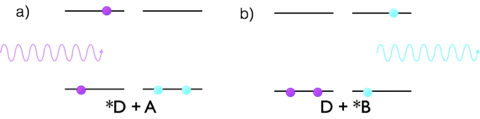
\includegraphics[width=0.7\linewidth]{images/forster} 

}

\caption{The mechanism of Förster resonance energy transfer. a) A donor molecule (purple) is excited by absorption of a photon into an excited state, there is a dipole dipole interaction with the acceptor molecule (blue) which is initially in the ground state. b) the product of energy transfer with the acceptor now in an excited state which is now capable of emission of a photon of lower energy.}\label{fig:forster}
\end{figure}

The first thing to note is that FRET is not a collisional process, energy is transferred between a donor and acceptor moiety at a distance, nor is this an emission of a photon by the donor and reabsorption of this photon by the acceptor.

FRET is a dipole dipole interaction where the acceptor quenches the excited state of the donor by energy transfer between the two moieties, figure \ref{fig:forster}, leaving the donor in an excited state which then decays as described in the a chapter on emission. This dipole-dipole interaction is a co-alligning of the transition dipole moments (see page Section @ref(\#sec:transdipole) on the donor and acceptor molecules - this gives a large dependence on the orientation factors of these two dipoles, the term κ in equation \eqref{eq:rateelectron}. In order for there to be an energy transfer there has to be an overlap between the emission spectra of the donor and the absorption spectra of the acceptor (equation \eqref{eq:overlap}), the greater, as illustrated in figure \ref{fig:overlapintegral}; this is in effect the overlap between the wave function of the excited state donor and the wave function of the ground state donor. The greater this overlap the more efficient the the energy transfer.

\begin{figure}

{\centering 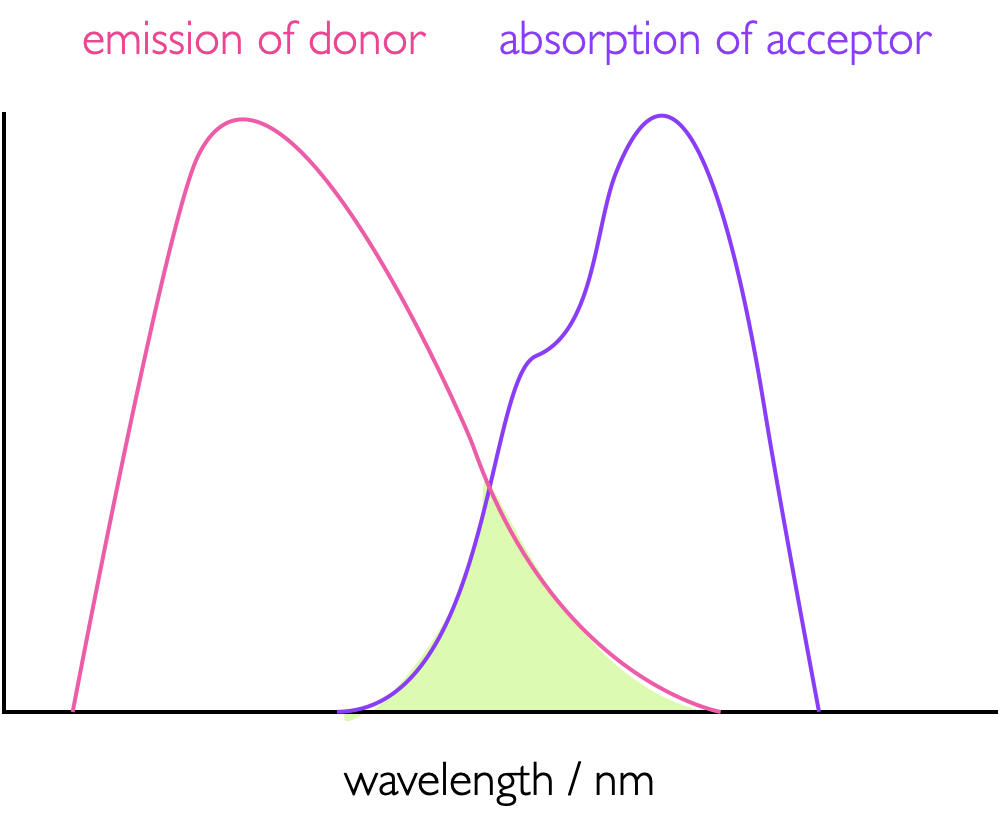
\includegraphics[width=0.7\linewidth]{images/overlapintegral} 

}

\caption{The overlap integral, J, (green shaded area) between the emission spectrum of a donor and absorption spectrum of an acceptor as used in FRET, the greater this overlap integral more more efficient the energy transfer.}\label{fig:overlapintegral}
\end{figure}

\begin{equation}
J (\bar \nu) = \int_0^\infty I_D(\bar \nu)\varepsilon_A(\bar \nu)\textrm{d}\bar \nu
\label{eq:overlap}
\end{equation}

The rate of Förster resonance energy transfer has been found empirically to depend upon a number of factors in addition to the overlap integral, \(J\), such as refractive index of the solvent, \(n\), and the dipole orientation factor \(\kappa\) (equation \eqref{eq:rateelectron}). Perhaps more obviously it also depends upon the separation of donor and acceptor, \(r\), quantum yield of emission of the donor, \(\phi_D\), and the unquenched lifetime of the donor molecule, \(\tau_D\).

\begin{equation}
k_{ET}= \frac{\phi_D \kappa^2}{\tau_D r^6}\frac{9 \ln 10 e^4}{128 \pi^5 N_A n^4}J
\label{eq:rateelectron}
\end{equation}

However, equation \eqref{eq:rateelectron}, is not simple to use, nor particularly descriptive and a simplified version of the equation tends to be used which has defined a `Förster radius', \(R_0\), equations 23 \& 24. The Förster radius is the radius at which half of the emission is quenched by the acceptor.

\begin{equation}
R_0^6=\frac{9 \ln 10 e^4 \phi_D \kappa^2}{128 \pi^5 N_A n^4 }J
\label{eq:forsterdistance}
\end{equation}

\begin{equation}
k_{ET}=\frac{1}{\tau_D}\frac{R_0^6}{r^6}
\label{eq:forstersimplified}
\end{equation}

Förster distances tend to be between 20 - 90 Å, and due to the parity of this with the size of biological macromolecules FRET is an excellent technique for studying biomolecules.
The quantum yield of Förster energy transfer, \(Φ_{ET}\) (equation \eqref{eq:QYET}), is usually just given the symbol \(E\), for efficiency. As described in equations \eqref{eq:rateelectron} - \eqref{eq:forstersimplified} this can be defined by:

\begin{equation}
\phi_ET = \frac{k_ET}{k_f^0+k_{ic}+ k_{ST}+k_{ET}}
\label{eq:QYET}
\end{equation}

By combining equations \eqref{eq:forstersimplified} \& \eqref{eq:QYET} it becomes easy to see how the efficiency of Förster energy transfer (\(E\) or \(Φ_{ET}\)) depends upon the distance, and we can see that the efficiency of energy transfer is 0.5 at the Förster distance. Figure \ref{fig:forsterdistance} sketches the distance dependence of efficiency of energy transfer, where it can be seen that at twice the Förster distance the efficiency has dropped almost to 0.

\begin{figure}

{\centering 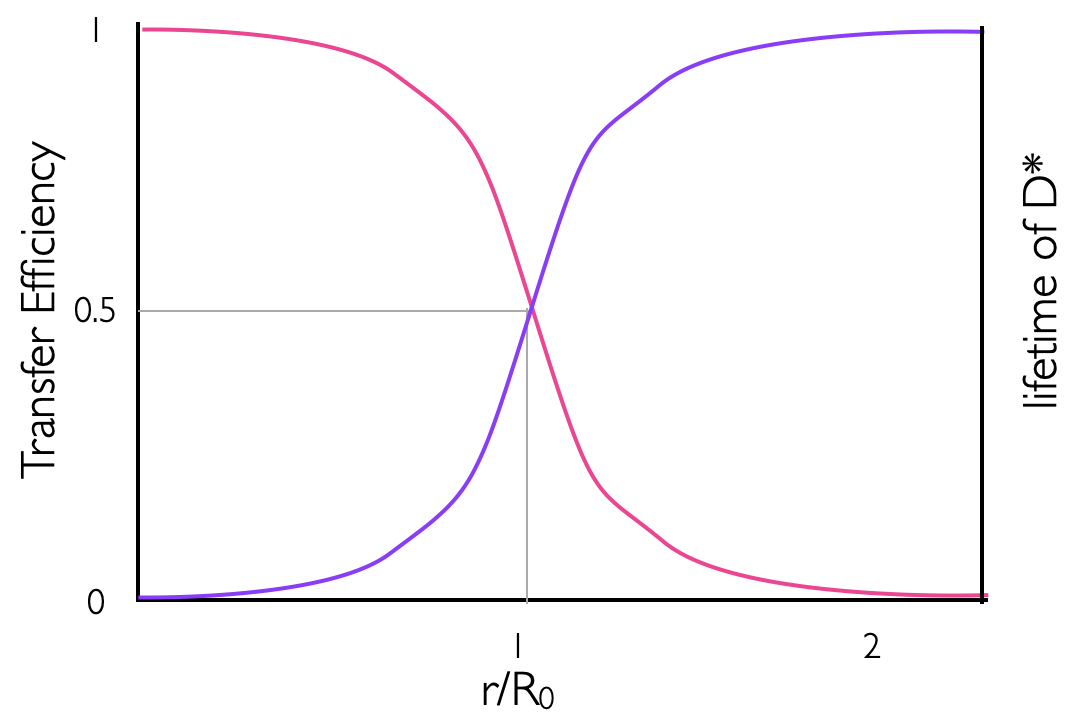
\includegraphics[width=0.7\linewidth]{images/forsterdistance} 

}

\caption{The distance dependence on the efficiency of energy transfer between a donor and acceptor in Förster resonance energy transfer (pink line), the purple line represents the distance dependence variation in the measured lifetime of the donor molecule with a maximum value of the unquenched donor of τ~D~..}\label{fig:forsterdistance}
\end{figure}

\begin{equation}
E=1-\frac{\tau_{DA}}{\tau_D}
\label{eq:efflifetime}
\end{equation}

\begin{equation}
E = \frac{R_0^6}{R_0^6+ r^6}
\label{eq:effdistance}
\end{equation}

The efficiency of energy transfer is calculated by measuring the quenched and unquenched fluorescence lifetime of the donor molecule. More detailed derivations of equations \eqref{eq:efflifetime} \& \eqref{eq:effdistance} may be found in Turro, Principles of Molecular Photochemistry.

Experimentally the process is confirmed to energy transfer at a distance, and not collisional energy transfer, as the rate constant of energy transfer \(k_{ET}\) is independent of solvent viscosity (as seen in equation \eqref{eq:diffcontrol} \& Stern-Volmer kinetics) and rates can be significantly higher than the rate limiting diffusion controlled rates. The energy is transferred by a dipole-dipole interaction.

\hypertarget{sec:Dexter}{%
\section{Dexter Energy Transfer}\label{sec:Dexter}}

Forster resonance energy transfer transfers energy between a donor an acceptor moiety by a dipole dipole interaction, however there is a second method of energy transfer which takes place by a slightly different mechanism. Dexter energy transfer transfers energy from a donor to acceptor moiety by a concerted exchange of electrons between the chromophores, figure \ref{fig:Dexter}.

\begin{figure}

{\centering 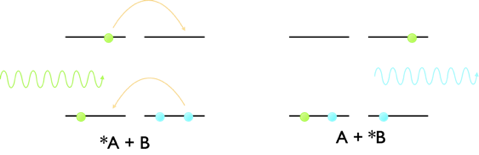
\includegraphics[width=0.7\linewidth]{images/Dexter} 

}

\caption{ The mechanism of Dexter energy transfer, where there is a concerted exchange of electrons from the LUMO of the donor to the empty LUMO of the acceptor and at the same time from the HOMO of the acceptor to the HOMO of donor. The two electrons move at the same time leading to a net exchange of energy from the donor to acceptor.}\label{fig:Dexter}
\end{figure}

The rate of Dexter energy transfer is again distance dependent and again is dependent upon the overlap integral, J, between the emission of the donor and the absorption of the acceptor (figure \ref{fig:overlapintegral}, equation \eqref{eq:overlap}). The rate of Dexter energy transfer is given by:

\begin{equation}
k_{ET}=KJe^{-\frac{2r}{L}}
\label{eq:ratedexter}
\end{equation}

where \(J\) is the overlap integral, \(K\) an empirical constant, \(r\) the separation between the donor and acceptor, and \(L\) another constant which represents the closest possible separation of the donor and acceptor (the sum of the van der Waals radii of the two chromophores).

From examining equation \eqref{eq:ratedexter} it can be seen that the rate of Dexter energy transfer decreases rapidly with increasing separation of donor and acceptor and occurs daily at distances less than 20 Å. Dexter energy transfer is the most dominant mechanism of triplet-triplet quenching.

\hypertarget{sec:tripletannihilation}{%
\section{Triplet-Triplet Annihilation}\label{sec:tripletannihilation}}

Excited state triplets are long lived, due to the spin-forbidden relaxation pathways back to the \(S_0\) state. However, there is a deactivation pathway that occurs by annihilation of two triplet states leading to formation of an excited state singlet and a ground state singlet.

\begin{figure}

{\centering 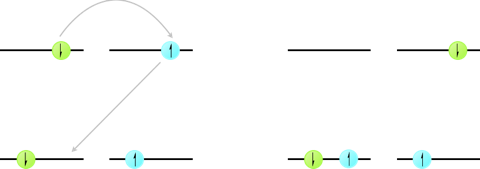
\includegraphics[width=0.7\linewidth]{images/triplettriplet} 

}

\caption{The mechanism of triplet triplet annihilation by Dexter energy transfer, concerted electron exchange between a donor and acceptor molecule leading to formation of a singlet excited state on one molecule and a ground state singlet on the other molecule.}\label{fig:triplettriplet}
\end{figure}

\begin{equation*}
^\ast D_{T_1}+^\ast D_{T_1} \longrightarrow ^\ast D_{S_1} + D_{S_0}
\end{equation*}

Triplet-triplet annihilation is the reason that quantum yields of phosphorescence are almost never unity (1).

\hypertarget{sec:O2quench}{%
\section{Quenching by Molecular Oxygen}\label{sec:O2quench}}

\begin{figure}

{\centering 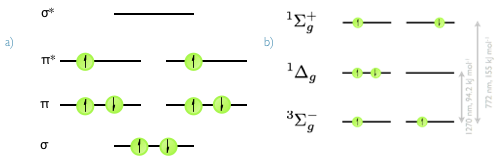
\includegraphics[width=0.7\linewidth]{images/O2} 

}

\caption{a) The valence set of molecular orbitals in molecular oxygen, showing the full electronic arrangement for the 3Σg− triplet ground state.  b) The π* HOMO orbital of molecular oxygen, with the 3Σg− triplet ground state and the singlet excited states 1Δg and 1Σg+.The relative energies of the two excited states are indicated.}\label{fig:O2}
\end{figure}

Molecular oxygen is unusual because it is a ground state triplet. It is an efficient quencher of excited triplet states because it has two accessible excited singlet states, figure \ref{fig:O2}. It is also capable of quenching excited singlet states, however since the quenching occurs by a Dexter mechanism the overlap integral between excited singlet states and ground state molecular oxygen tends to be very small leading to very small quantum yields of singlet oxygen formation.

\begin{equation}
\textrm{O}_2(^3 \Sigma _g^-)+ ^\ast \textrm{Dye}(T_1) \longrightarrow ^\ast \textrm{O}_2(^1 \Delta _g) + \textrm{Dye}(S_0)
\label{eq:O2quench}
\end{equation}

Usually the molecular oxygen is excited into the \^{}\textsuperscript{Σ\textsubscript{g}}+\^{} state, but this rapidly decays to the \textsuperscript{1}Δ\textsubscript{g} state. The \textsuperscript{1}Δ\textsubscript{g} is usually simply referred to as singlet oxygen and is relatively stable because of the spin forbidden deactivation, having a lifetime of a few µs in aqueous solvent and hours in the gas phase.

Chemically singlet oxygen formation is very interesting as it is extremely reactive, and has been shown to be an important factor in a number of mechanistic pathways leading to damage of DNA and proteins.

\hypertarget{before-completing-this-section-1}{%
\section{Before Completing this Section}\label{before-completing-this-section-1}}

To support the material in this section it is suggested you read chapter 6 of Wardle `Principles and Application of Photochemistry'.

\hypertarget{ch:Workshop3}{%
\chapter{Workshop Questions for Week 4}\label{ch:Workshop3}}

\hypertarget{sec:overlap}{%
\section{Short conceptual question - Electronic-vibrational overlap integrals}\label{sec:overlap}}

\begin{figure}

{\centering 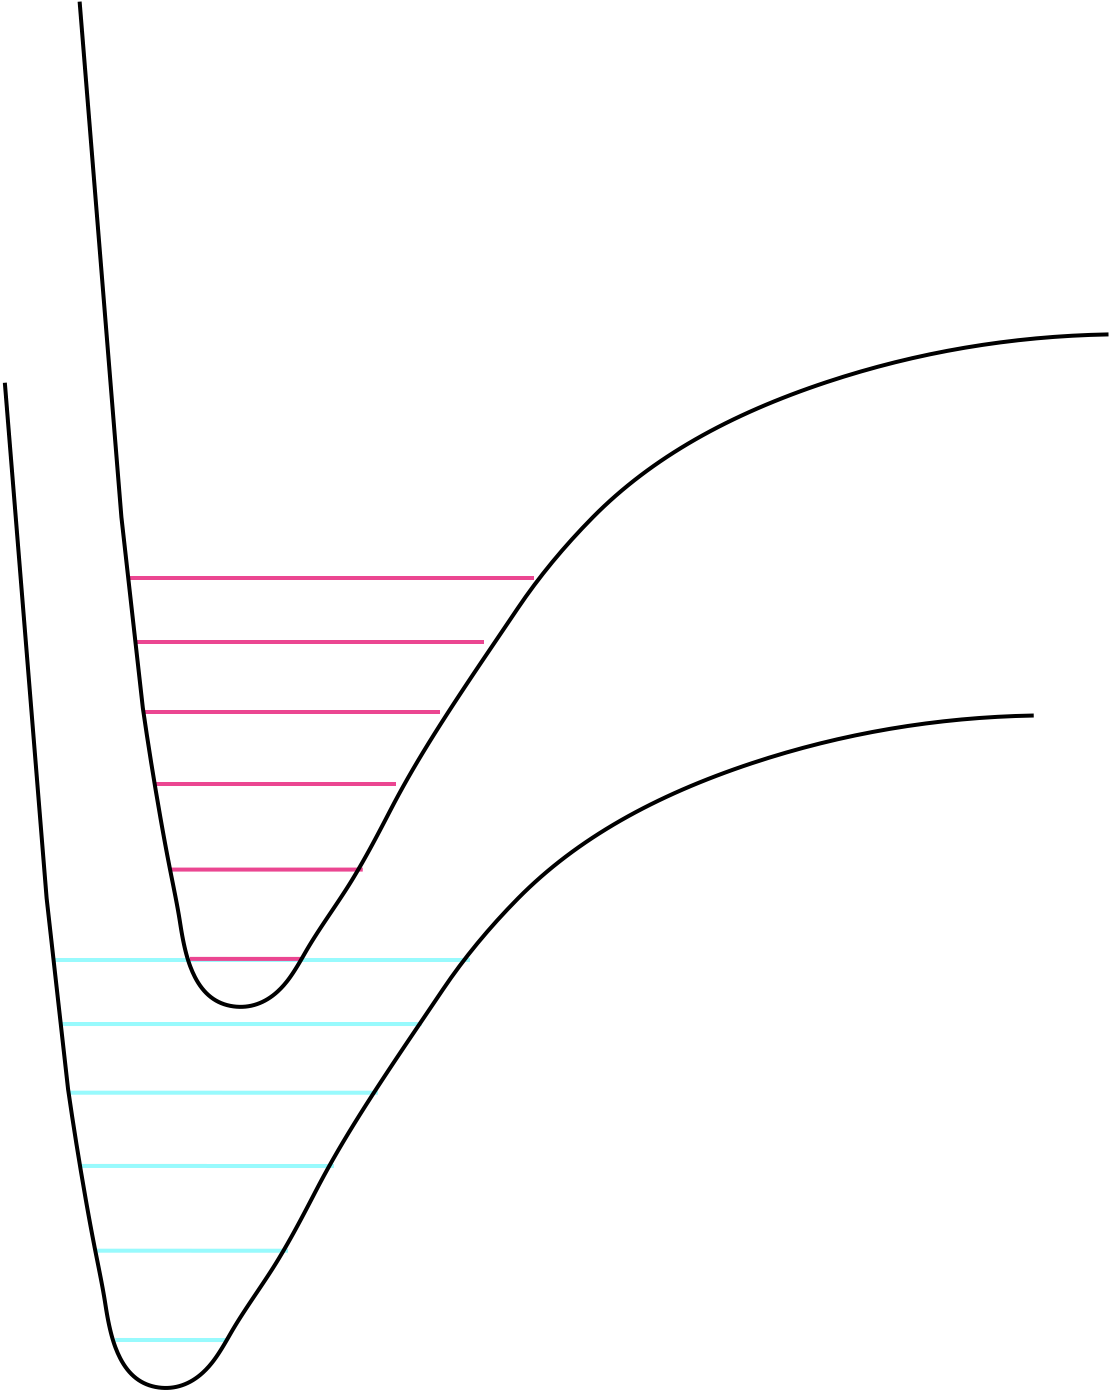
\includegraphics[width=0.7\linewidth]{images/overlap} 

}

\caption{The grond and excited state potential wells and the vibrational levels within them.}\label{fig:overlap}
\end{figure}

On the figure sketch the vibrational energy levels in the ground and the excited state.

How would the following affect this overlap integral?
1. Energy gap.
1. The vibrational energy gaps
1. Reaction coordinate (the difference in structure between ground and excited state)

\emph{(I will use drawing in UniDoodle to ask this in class, with the second part being a discussion question)}

\hypertarget{sec:structureQY}{%
\section{Short conceptual question - The effect of structural changes on quantum yield}\label{sec:structureQY}}

5,10-dihydroindeno{[}2,1-a{]}indene and trans-stilbene (figure \ref{fig:stilbeneindene}) are similar in structure but have very different fluorescent quantum yields of 1.00 and 0.05 respectively, however for trans-stilbene this increases to 0.75 at 77 K. Suggest a reason for the difference in quantum yield of:
- the two molecules
- the two temperatures

\begin{figure}

{\centering 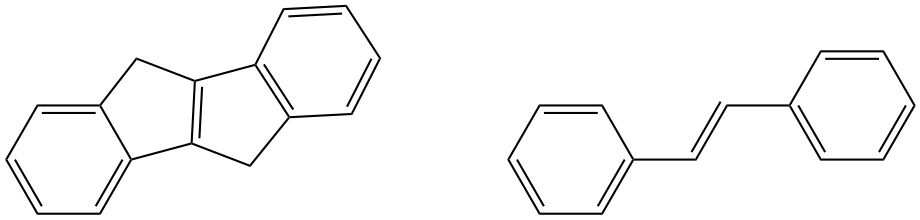
\includegraphics[width=0.6\linewidth]{Images/stilbeneindene} 

}

\caption{5,10-dihydroindeno[2,1-a]indene (left) and trans-stilbene (right)}\label{fig:stilbeneindene}
\end{figure}

\emph{(This will be a discussion question)}

\hypertarget{sec:ratephos}{%
\section{Short mathematical question - Effect of the rate of singlet triplet intersystem crossing on th quantum yield of phosphorescence}\label{sec:ratephos}}

Why is it likely that the quantum yield of phosphorescence of a sample would increase after the sample is frozen.

\emph{(This will be a discussion question)}

\hypertarget{sec:calcphos}{%
\section{Short mathematical question - Determining the quantum yield of phosphorescence}\label{sec:calcphos}}

A molecule decays by a combination of internal conversion, intersystem crossing and phosphorescence. What is the quantum yield of phosphorescence?

\begin{itemize}
\tightlist
\item
  k\textsubscript{IC} = 2.1 × 10\textsuperscript{11} s\textsuperscript{−1}
\item
  k\textsubscript{ST} = 2.9 × 10\textsuperscript{9} s\textsuperscript{−1}
\item
  k\textsubscript{TS} = 7.4 × 10\textsuperscript{6} s\textsuperscript{−1}
\item
  k\textsubscript{p}\textsuperscript{o} = 6.2 × 10\textsuperscript{8} s\textsuperscript{−1}
\end{itemize}

\emph{(This will be a discussion question)}

\hypertarget{sec:exhydrocarbons}{%
\section{Short conceptual question - Deactivation of excited state aromatic hydrocarbsons}\label{sec:exhydrocarbons}}

\begin{longtable}[]{@{}llll@{}}
\caption{\label{tab:smallmolQY} The quantum yields of various deactivation processes in small organic molecules measured at 77 K in a glass matrix.}\tabularnewline
\toprule
& Φ\textsubscript{f} & Φ\textsubscript{ST} & ΔE / kJ mol\textsuperscript{−1}\tabularnewline
\midrule
\endfirsthead
\toprule
& Φ\textsubscript{f} & Φ\textsubscript{ST} & ΔE / kJ mol\textsuperscript{−1}\tabularnewline
\midrule
\endhead
Napthalene & 0.20 & 0.80 & 385\tabularnewline
Anthracene & 0.70 & 0.30 & 318\tabularnewline
Pyrene & 0.6 & low & 322\tabularnewline
Tetracene & 0.1 & 0.65 & 251\tabularnewline
Pentacene & 0.10 & 0.15 & 209\tabularnewline
\bottomrule
\end{longtable}

When examining the data above suggest why it is likely why the quantum yields of both fluorescence and singlet to triplet intersystem crossing decrease with increasing molecule size.

\emph{(This will be a discussion question)}

\hypertarget{sec:dsolvent}{%
\section{Short conceptual question - Affect of deuteration of solvents.}\label{sec:dsolvent}}

Singlet oxygen has a phosphorescence wavelength of around 1070 nm and a lifetime of 2 µs in water, how would you expect this lifetime to change for singlet oxygen in D\textsubscript{2}O?

\emph{(This will be a discussion question)}

\hypertarget{sec:isotope}{%
\section{Short conceptual question - Isotope effects on deactivation of an excited state}\label{sec:isotope}}

The fluorescence quantum yield and singlet state lifetime of both proteated and deuterated pyrene are 0.90 and 450 ns respectively. Why does deuteration of the sample have no measureable affect on these values?

Conversely for naphthalene phosphorescence (in glass at 77 K) the quantum yield of phosphoresce increases from 0.05 to \textasciitilde0.80 on deuteration of the sample. (ΔE = 251 kJ mol\textsuperscript{−1} ). Explain this observation with respect to the energy gap law.

\emph{(This will be a discussion question)}

\hypertarget{sec:heavy}{%
\section{Short conceptual question - The effect of heavy attoms on the rate of intersystem crossing}\label{sec:heavy}}

\begin{longtable}[]{@{}llll@{}}
\caption{\label{tab:heavyatom} The affect of substitution of different halogens on the rates of phosphorescence and singlet to triplet intersystem crossing.}\tabularnewline
\toprule
& k\textsubscript{p} & k\textsubscript{ST} & Φ\textsubscript{p} / Φ \textsubscript{f}\tabularnewline
\midrule
\endfirsthead
\toprule
& k\textsubscript{p} & k\textsubscript{ST} & Φ\textsubscript{p} / Φ \textsubscript{f}\tabularnewline
\midrule
\endhead
Napthalene & 0.05 & 0.39 & 0.09\tabularnewline
1-fluoronaphthalene & 0.23 & 0.42 & 0.07\tabularnewline
1-chloronaphthalene & 1.1 & 2.35 & 5.2\tabularnewline
1-bromonaphthalene & 13.5 & 36.5 & 169\tabularnewline
1-iodonaphthalene & 190 & 310 & \textgreater760\tabularnewline
\bottomrule
\end{longtable}

Briefly explain why the rates of these processes increase as we move down the group.

\emph{(This will be a discussion question)}

\hypertarget{sec:osphen}{%
\section{Short conceptual question - The effect of absorbance and emission wavelengths on the quantum yield of emission}\label{sec:osphen}}

\begin{longtable}[]{@{}llllll@{}}
\caption{\label{tab:osphen} The spectroscopic details of a family of osmium complexes.}\tabularnewline
\toprule
& λ\textsubscript{abs} / nm & λ\textsubscript{em} / nm & ΔE / eV & τ/ ns & Φ\textsubscript{em}\tabularnewline
\midrule
\endfirsthead
\toprule
& λ\textsubscript{abs} / nm & λ\textsubscript{em} / nm & ΔE / eV & τ/ ns & Φ\textsubscript{em}\tabularnewline
\midrule
\endhead
{[}Os(phen)\textsubscript{3}{]}\textsuperscript{2+} & 650 & 720 & 0.186 & 260 & 0.016\tabularnewline
{[}Os(phen)\textsubscript{2}(dppene){]}\textsuperscript{2+} & 455 & 609 & 0.69 & 1830 & 0.138\tabularnewline
{[}Os(phen)(dppene)\textsubscript{2}{]}\textsuperscript{2+} & 400 & 530 & 0.761 & 3600 & 0.518\tabularnewline
\bottomrule
\end{longtable}

Why does the fluorescence lifetime increase as the phenanthroline ligands are replaced with dppene ligands?

\emph{(This will be a discussion question)}

\hypertarget{ch:excited}{%
\chapter{Other Excited State Systems}\label{ch:excited}}

\hypertarget{sec:exitedLOs}{%
\subsection{Learning Objectives}\label{sec:exitedLOs}}

At the end of this section you should be able to:

\begin{itemize}
\tightlist
\item
  Explain the origin of excimer and exciplex emission spectra.
\item
  Describe why excimer and exciplex formation are concentration dependent.
\item
  Interpret changes in emission spectra with changing concentration to justify formation of either excimers or exciplexes.
\item
  Show an awareness of excited state reactions and rearrangements.
\end{itemize}

\hypertarget{sec:excimers}{%
\section{Excimers}\label{sec:excimers}}

An excimer is an excited state dimer formed between two identical molecules. A photon is delocalised between two molecules which in the excited state are weakly bound together. Excimers are relatively long lived species, and were first noticed when increasing the concentration of certain fluorophores.

It was found that upon increasing the concentration of the chromophore the fluorescence did not increase linearly, and upon reaching higher concentrations the fluorescence decreased; however, this decrease in fluorescence occurred with an increase in a new emission band of lower energy. Excimer bands tend to be broad featureless and Gaussian in profile, figure 33. It is important to note that there is no bonding between the chromophores in the ground state; excimers only occur at high concentrations as an excited state molecule has to interact with a second ground state molecule in the lifetime of the excited state. There is no change in the absorption of the sample (as there is only excitation of monomer species), only formation of a new band in the emission spectrum.

Excimers exist because of formation of a weak bond between the two chromophores as shown in figure \ref{fig:excimer}. By formation of this bond any emission from the excimer has to be lower in energy than the fluorescence of the monomer chromophore. The ground state consists of two molecules in an dissociated state, upon emission from the excimer the structure of the excimer remains (as with the Stokes shift) and the two molecules diffuse apart.

It is important to note that there is no charge separation in the excimer and that the excited state is shared across both molecules.

\begin{figure}

{\centering 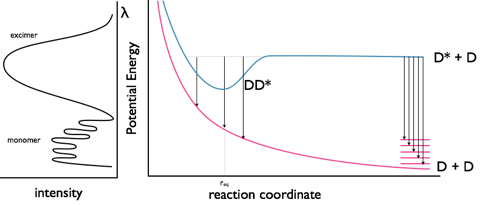
\includegraphics[width=0.7\linewidth]{images/excimer} 

}

\caption{The monomer and excimer emission of pyrene, and an energy level profile showing the fluorescence from the non-bonded D* state as well as the excimer emission from the DD* state.}\label{fig:excimer}
\end{figure}

\begin{figure}

{\centering 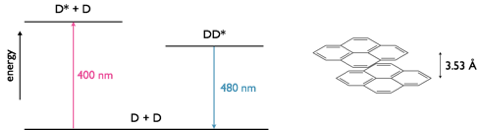
\includegraphics[width=0.7\linewidth]{images/pyreneexcimer} 

}

\caption{A pyrene excimer with a separation of 3.53 Å between the two planes of nuclei, in the excited state dimer the two ring systems of pyrene have a weak interaction between them. The emission maxima of fluorescence is 400 nm whereas the emission maxima for the excimer is 480 nm.}\label{fig:pyreneexcimer}
\end{figure}

A concept bite video briefly covering the concepts of eximers and exciplexes (video length 7m05s)

\hypertarget{exciplexes}{%
\section{Exciplexes}\label{exciplexes}}

Excimers consist of an excited state shared between two identical monomer units, whereas exciplexes are excited state complexes of two different chromophores. Due to the differences in molecular orbitals of the chromophores exciplexes have a dipole across the excited state complex; this dipole can lead to formation of a charge separated species, figure \ref{fig:exciplex}.

Exciplexes can undergo emission from this state, leading to formation of dissociated monomer units or there can be a solvent reorganisation leading to formation of a solvent separated radical ion pair, at this point there can still be charge recombination and relaxation of the system (this time with the excess energy lost as heat) to the original monomer chromophore units.

\begin{figure}

{\centering 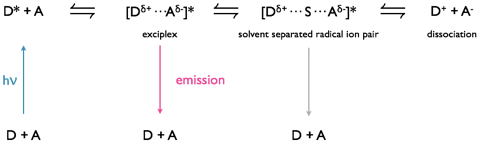
\includegraphics[width=0.7\linewidth]{images/exciplex} 

}

\caption{Formation of an exciplex from an excited state donor and ground state acceptor chromophore. The exciplex has a small charge separation leading to a dipole over the excited state complex, under some circumstances with the introduction of solvent between the chromophores in the exciplex this can then go on to form a solvent separated radical ion pair which may then go on to form a charge separated redox pair.}\label{fig:exciplex}
\end{figure}

\begin{figure}

{\centering \includegraphics[width=0.7\linewidth]{images/exciplexenergy} 

}

\caption{Energy profile of exciplex formation showing the lower energy state of the exciplex over the D* + A system. Emission from the exciplex is lower energy than fluorescence from the monomer donor chromophore.}\label{fig:exciplexenergy}
\end{figure}

Exciplexes are common in organic solvent as non polar solvents are not good at stabilising ions in solution, as the polarity of the solvent increases then the charge separated state becomes more favoured. Exciplexes and other charge separated species are of interest in chemistry for use in molecular wires and energy storage devices.

Please see video above in Section \ref{sec:excimers} for a review of this topic (timecode 4m52s).

\hypertarget{sec:photoinducedisom}{%
\section{Photoinduced Isomerisation}\label{sec:photoinducedisom}}

When discussing the absorption of light it was noted that by promotion of an electron into an anti-bonding orbital the bond order was reduced. In the case of double (π) bonds in molecules such as retinal (figure), the bond order of one of the double bonds is reduced and therefore allows rotation around this now single bond, as the energy is lost (either by internal conversion or emission) the π-bond is restored. A simple Lewis model of bonding is convenient, however we have to consider the molecular orbital, and this version of bonding highlights a particular bond which is weakened in the excited state, consequently rotation occurs around a specific bond in a conjugated chain.

\begin{figure}

{\centering \includegraphics[width=0.7\linewidth]{images/retinal} 

}

\caption{The cis-trans isomerisation of retinal, which when combined with the protein rhodopsin is vital in vision. Absorption of a photon, reduces the bond order of a specific bond due to characteristics of the excited state molecular orbital.}\label{fig:retinal}
\end{figure}

The steady state photochemical yield of any such cis-trans isomerisation will depend upon the absorption of each of the chromophore isomers at the excitation wavelength, the composition of this steady state is referred to as the photostationary state. The composition of this photostationary state may be easily calculated making only minor assumptions.

The most important of these assumptions is that when in the excited state there is an equal probability that the molecule will relax to the cis \& trans states. The second assumption is that (near) monochromatic light is used, because we have already seen that the molar extinction coefficient is very wavelength dependent. Finally the excitation has to occur long enough for the (steady state) photostationary state to be established.

Figure \ref{fig:cistransstilbene} shows the absorption spectra of the two isomers of stilbene, there are a number of interesting photophysical details about this molecule, but it should be noted that the molar extinction coefficient is different for each of the isomers. The point where the two spectra cross is called the isobestic point , for stilbene this is 288 nm, if the system is excited at this wavelength then the yield of each isomer will be the same. However at all other wavelengths the yield of one isomer will be higher than the other. If an excitation wavelength is used whereby the molar extinction coefficient of the trans isomer is highest then this isomer is excited preferentially and there is less of this isomer is the photostationary state.

\begin{figure}

{\centering \includegraphics[width=0.6\linewidth]{images/cistransstilbene} 

}

\caption{The absorption spectra of trans \& cis stilbene in hexane.}\label{fig:cistransstilbene}
\end{figure}

In summary the higher the molar absorption coefficient at the excitation wavelength the lower the yield of that product in the photostationary state.

The dynamics of cis-trans isomerisation may be studies by using some of the photophysics already discussed. Figure \ref{fig:cisquench} shows a cis / trans system, in the cis position the emission from a fluorophore is quenched so there is no visible emission from the dye. In the trans position position of the quencher now means that there is either no quenching or the quenching is greatly reduced, consequently the emission from the fluorophore is greatly increased.

\begin{figure}

{\centering \includegraphics[width=0.2\linewidth]{images/cisquench} 

}

\caption{The quenching of emission of a fluorophore by a nearby quencher, in the cis configuration the emission from the fluorophore is completely quenched, whereas in the trans configuration emission from the fluorophore is observed.}\label{fig:cisquench}
\end{figure}

\hypertarget{before-completing-this-section-2}{%
\section{Before Completing this Section}\label{before-completing-this-section-2}}

To support the material in this section it is suggested you read pages 90-96 of Wardle `Principles and Application of Photochemistry'.

\hypertarget{ch:Workshop4}{%
\chapter{Workshop Questions for Week 5}\label{ch:Workshop4}}

\hypertarget{sec:diffcontrol}{%
\section{Short mathematical question - Determining rates of diffusion controlled quenching}\label{sec:diffcontrol}}

The rate of diffusion (\(k_d\)) in solution is given by equation \eqref{eq:diffcontrolrate}, where \(\eta\) is the viscosity of the solution.

\begin{equation}
k_d = \frac{8RT}{3 \eta}
\label{eq:diffcontrolrate}
\end{equation}

Determine the maximum possible rate of diffusion controlled quenching at 20 ºC in:

\begin{enumerate}
\def\labelenumi{\alph{enumi}.}
\tightlist
\item
  water (\(\eta=\) 1.0016 mPa s)
\item
  methanol (\(\eta=\) 0.594 mPa s)
\end{enumerate}

\emph{(I will use UniDoodle to ask this in class)}

\hypertarget{sec:emintquench}{%
\section{Short mathematical question - Determining the effect of diffusion controlled quenching on emission intensity}\label{sec:emintquench}}

What emisison intensity would you expect if 50 mM of a quencher quenches the emission of a chromophore dissolved in basic ethanol at 10 ºC, with natural lifetime of 13.2 ns and emission quantum yield, Φ\textsubscript{f}, of 0.32, if the unqunched intensity is 35240.

\(\eta\)\textasciitilde EtOH, 10 ºC\textasciitilde{} = 1.394 mPa s

\emph{(This will be a discussion question)}

\hypertarget{sec:temp}{%
\section{Short conceptual question - effect of temperature}\label{sec:temp}}

YO-Pro-1 is quenched in the presence of molecular oxygen, as the temperature increases this quenching increases, what does this indicate about the mechanism of quenchign and why?

\emph{(This will be a discussion question)}

\hypertarget{short-conceptual-question---change-in-behaviour-on-freezing}{%
\section{Short conceptual question - change in behaviour on freezing}\label{short-conceptual-question---change-in-behaviour-on-freezing}}

As the concentration of a species increases the wavelength of emission increases in the solution phase but this same shift in wavelength is not when the solution is frozen. What photochemical process may be occuring to explain this effect?

\emph{(This will be a discussion question)}

\hypertarget{sec:static_question}{%
\section{Short conceptual question - static quenching}\label{sec:static_question}}

When in the presence of a quencher the intensity of emission of a chromophore (τ\textsubscript{0} = 5.2 ns) was reduced from 4200 cps to 2100 cps at 25 ºC and 1800 cps at 10 ºC. What would the lifetime of the quenched chromophore be at 25 ºC?

\emph{(This will be a discussion question)}

\hypertarget{short-conceptual-question---isoemissive-point}{%
\section{Short conceptual question - isoemissive point}\label{short-conceptual-question---isoemissive-point}}

As the concentration of pyrene dissolved in toluene increases a new broad band with a broad featureless spectrum is observed, which is from excimer emisison. What evidence is there that emission is only from single molecule and excimer emission and no other states?

How would the absorption spectrum change as the concentration increases?

\begin{figure}

{\centering \includegraphics[width=0.3\linewidth]{images/pyrene} 

}

\caption{The emission spectrum of pyrene in tolune as low (solid line) and higher (dotted lines) concentrations.}\label{fig:pyrene}
\end{figure}

\hypertarget{sec:static2}{%
\section{Short conceptual question - static quenching}\label{sec:static2}}

10-methylacridinium chloride (MAC) is quenced in the presence of adenosine monophosphate (AMP, figure (\ref{fig:AMP})). The effect of quenching is enhanced by addition of sodium sulfate.

In a separate experiment the emssion of MAC is unaffected by addition of sodium sulfate (when not in the presence of AMP).

Suggest the mechanism of quenching, justifying this with reference to the experimental data.

\begin{figure}

{\centering \includegraphics[width=0.3\linewidth]{images/MAC} 

}

\caption{The structure of methyl acridinium.}\label{fig:MAC}
\end{figure}

\begin{figure}

{\centering \includegraphics[width=0.3\linewidth]{images/AMP} 

}

\caption{The structure of adenosine monophosphate.}\label{fig:AMP}
\end{figure}

\emph{(This will be a discussion question)}

\hypertarget{sec:acridone}{%
\section{Long mathematical question - Quenching of emission of acridone}\label{sec:acridone}}

Acridone (figure \ref{fig:acridone})is found to be quenched in the presence of potassium iodide in aqueous solution at 26 oC. Solutions were maintained at constant ionic strength by use of KNO2, the KNO2 does not affect the emission intensity of the solution.

\begin{figure}

{\centering \includegraphics[width=0.3\linewidth]{images/acridone} 

}

\caption{The structure of acridone.}\label{fig:acridone}
\end{figure}

The following data were collected for the emission of acridone.

\begin{longtable}[]{@{}cccc@{}}
\caption{\label{tab:acridonequench} The effect of potassium iodide concentration on emission intensity and fluorescence lifetime of acridone in aqueous solution.}\tabularnewline
\toprule
{[}KI{]} / M & {[}KNO\textsubscript{2}{]} / M & Emission intensity / arb & τ / ns\tabularnewline
\midrule
\endfirsthead
\toprule
{[}KI{]} / M & {[}KNO\textsubscript{2}{]} / M & Emission intensity / arb & τ / ns\tabularnewline
\midrule
\endhead
0 & 1.100 & 16580 & 17.60\tabularnewline
0.040 & 1.060 & 3753 & 3.90\tabularnewline
0.100 & 1.000 & 1566 & 1.80\tabularnewline
0.200 & 0.900 & 721 & 0.95\tabularnewline
0.300 & 0.800 & 446 & 0.64\tabularnewline
0.500 & 0.600 & 242 & 0.39\tabularnewline
0.800 & 0.300 & 121 & 0.25\tabularnewline
\bottomrule
\end{longtable}

\begin{enumerate}
\def\labelenumi{\arabic{enumi}.}
\item
  Using an appropriate plot (or plots) determine if the quenching is static, dynamic or a combination of both mechanisms.
\item
  Determine any relevant quenching constants (k\textsubscript{d} and/or K\textsubscript{S} )
\end{enumerate}

\emph{(This will be a discussion question)}

\hypertarget{ch:Workshop5}{%
\chapter{Workshop Questions for Week 6}\label{ch:Workshop5}}

\hypertarget{sec:O2quench_question}{%
\section{Short conceptual question - O2 quenching}\label{sec:O2quench_question}}

\begin{enumerate}
\def\labelenumi{\arabic{enumi}.}
\item
  Given molecular oxygen has an emission with λ\textsubscript{max} around 1280 nm why is it such a good quencher of excited states?
\item
  Why is the efficiency of quenching lower for excited singlet states?
\end{enumerate}

\emph{Are you all happy with the energy level diagram of molecular oxygen?}

\emph{(This will be a discussion question)}

\hypertarget{sec:FRET}{%
\section{Short mathematical question - Förster resonance energy transfer}\label{sec:FRET}}

A donor, D, with an unquenched lifetime of 5.0 ns, was found to have a steady state emission intensity of 20.5 in free solution and 4.1 when in the presence of a quencher, Q. Assuming the Förster distance is 50 Å determine :

\begin{enumerate}
\def\labelenumi{\arabic{enumi}.}
\tightlist
\item
  the transfer efficiency, E.
\item
  the lifetime of D in the presence of the quencher Q
\item
  the equilibrium separation of D \& Q
\item
  the rate constant for energy transfer
\end{enumerate}

\emph{(This will be a discussion question)}

\hypertarget{sec:FRETdist}{%
\section{Short conceptual quesiton - Förster distance}\label{sec:FRETdist}}

Determine the quantum yield of emission of the donor in a FRET pair system where donor and acceptor are separated by the Förster distance, the lifetime of the unquenched system is 8.4 ns. The unquenched quantum yield is 0.58*

\emph{(I will poll this question on UniDoodle and then maybe discuss some of the responses)}

\hypertarget{short-conceptual-question---redox-chemistry}{%
\section{Short conceptual question - redox chemistry}\label{short-conceptual-question---redox-chemistry}}

Why does formation of an excited state decrease both the oxidation and reduction potential of a species?

\hypertarget{sec:donoracceptor}{%
\section{Short conceptual quesiton - Donor-accceptor system}\label{sec:donoracceptor}}

In a single molecule study of a donor bound to an acceptor via a flexible, short aliphatic chain it was found that lifetime of the excited state varied (time beween single photon detection of emission after an excitation pulse). Suggest why this is the case.

\emph{(This will be a discussion question)}

\hypertarget{sec:ruquench}{%
\section{Short conceptual quesiton - Quenching of ruthenium}\label{sec:ruquench}}

Ruthenium tris bipyridine {[}Ru(bpy)\textsubscript{3}{]}\textsuperscript{2+} has a λ\textasciitilde max, abs\textasciitilde{} = 470 nm and λ\textasciitilde max, em\textasciitilde{} = 465 nm. The natural lifetime is 13.6 µs.

Suggest why molecular oxygen is an efficient quencher of the emmission of {[}Ru(bpy)\textsubscript{3}{]}\textsuperscript{2+}.

\emph{(This will be a discussion question)}

\hypertarget{sec:spectra}{%
\section{Short conceptual question - Energy transfer and spectra}\label{sec:spectra}}

How would you expect the absorption and emission spectra observed in an experiment to change when an emmisive acceptor is added?

If you keep the emisison wavelength the same and scan the intensity of this band with changing excitation wavelength how will this (excitation) spectrum vary from the absorbance and how can it be used to confirm energy transfer?

\emph{(This will be a discussion question)}

\hypertarget{sec:FRETDNA}{%
\section{Short conceptual question - Effect of separation}\label{sec:FRETDNA}}

A `cyanine-3' and `cyanine-5' are cyanine dyes which are frequently used as markers in experiments with DNA.

Cyanine-3 has a λ\textasciitilde max, abs\textasciitilde{} = 554 nm and λ\textasciitilde max, em\textasciitilde{} = 568 nm

Cyanine-5 has a λ\textasciitilde max, abs\textasciitilde{} = 649 nm and λ\textasciitilde max, em\textasciitilde{} = 666 nm

In an experiment they are tethered to either end of a DNA oligomer of 4, 5, 6, 7, 8, 9, 10 11 \& 12 base pairs. However the pattern expected of increasing lifetime as the separation increased was not observed. Suggest why this may be occuring.

\emph{(This will be a discussion question)}

\hypertarget{short-conceptual-question---lifetimes}{%
\section{Short conceptual question - lifetimes}\label{short-conceptual-question---lifetimes}}

The emission spectra of 2-phenylindole shows a marked difference with changes in concentration.

At a concentration of 1 × 10\textsuperscript{−5} M the measured lifetime is 0.86 ns, whereas at 5 × 10\textsuperscript{−3} M the measured lifetime is 3.42 ns.

\begin{figure}

{\centering \includegraphics[width=0.3\linewidth]{images/phenylindole} 

}

\caption{The emission spectrum of pyrene in tolune as low (solid line) and higher (dotted lines) concentrations.}\label{fig:phenylindole}
\end{figure}

Why does the measured lifetime depend upon concentration?

\emph{(This will be a discussion question)}

\hypertarget{short-conceptual-question---effect-of-time-delay}{%
\section{Short conceptual question - effect of time delay}\label{short-conceptual-question---effect-of-time-delay}}

If a solution of pyrene in cyclohexane is excited with a very short (ps) pulse of lightafter 1 ns the emission spectrum observed is mainly that of the momomer, whereas after 100 ns emission is principally from the excimer. Why is this the case?

\emph{(This will be a discussion question)}

  \bibliography{book.bib,packages.bib}

\end{document}
